\documentclass[oneside,a4paper,11pt]{book}
\usepackage[utf8]{inputenc}
\usepackage{svg}
\usepackage[italian]{babel}
\usepackage{float}
\usepackage{fancyvrb}
\usepackage{titling}
\usepackage[margin=1in,footskip=0.25in]{geometry}
\usepackage{listings}
\usepackage[DIV=12,BCOR=2mm,headinclude=true,footinclude=false]{typearea}
\usepackage{color, colortbl,xcolor}
\usepackage[hidelinks]{hyperref}
\usepackage{tcolorbox}
\usepackage{chngcntr}
\usepackage{diagbox}
\usepackage{calc}
\usepackage{amssymb}
\usepackage{subcaption}
\usepackage{amsthm}
\usepackage{amsfonts}
\usepackage{mathtools}
\usepackage{parskip}
\usepackage{cancel}
\usepackage{forest}
\usepackage{listings}
\usepackage{mathrsfs}
\usepackage{enumitem}
\usepackage{makecell}
\usepackage{tikz}
\usepackage{pgfplots}
\usepackage{algpseudocode}
\usepackage[operators,sets]{cryptocode}
\usepackage{tikzpeople}
\newcommand{\probP}{\text{I\kern-0.15em P}}
\pgfplotsset{compat=1.18}
\usepackage{fancyhdr}
\fancypagestyle{plain}{\fancyhf{}\renewcommand{\headrulewidth}{0pt}}
\pagestyle{fancy}
\fancyhf{}% Clear header/footer
\fancyhead[L]{\nouppercase\leftmark}
\fancyhead[R]{\thepage}
\usetikzlibrary{positioning,shapes.geometric,arrows.meta,matrix,automata,decorations.pathmorphing,patterns,
decorations.pathreplacing,shapes.multipart,calc,snakes,graphs,graphs.standard}

\usetikzlibrary{arrows.meta, backgrounds, chains, positioning, shapes.geometric, shapes.multipart}
\tcbuselibrary{skins}
\counterwithin{figure}{section}
%Nuovi comandi
\newcommand\myeq{\stackrel{\mathclap{\normalfont\mbox{def}}}{=}}
\newcommand\prodG{\stackrel{\mathclap{\normalfont\mbox{\tiny{G}}}}{\Longrightarrow}}
%asmthm
\newlength{\marginlabelsep}\setlength{\marginlabelsep}{0.5em}
\newtheoremstyle{italicstyle} %% Name
  {} %% <- Space above (empty = default = \topsep = 8.0pt plus 2.0pt minus 4.0pt)
  {} %% <- Space below (empty = default = \topsep = 8.0pt plus 2.0pt minus 4.0pt)
  {\itshape} %% <- Body font
  {} %% <- Indent amount (empty = no indent, \parindent = just that)
  {\bfseries} %% <- Thm head font
  {} %% <- Punctuation after thm head
  {1pt} %% <- Space after thm head (or " " or \newline) (default: 5pt plus 1pt minus 1pt)
  {\vtop to 0pt{\llap{\thmname{#1}\hskip\marginlabelsep}
                \llap{\thmnumber{#2}\hskip\marginlabelsep}}\thmnote{#3\\}%
  }
\newtheoremstyle{normStyle} %% Name
  {} %% <- Space above (empty = default = \topsep = 8.0pt plus 2.0pt minus 4.0pt)
  {} %% <- Space below (empty = default = \topsep = 8.0pt plus 2.0pt minus 4.0pt)
  {\normalfont} %% <- Body font
  {} %% <- Indent amount (empty = no indent, \parindent = just that)
  {\bfseries} %% <- Thm head font
  {} %% <- Punctuation after thm head
  {1pt} %% <- Space after thm head (or " " or \newline) (default: 5pt plus 1pt minus 1pt)
  {\vtop to 0pt{\llap{\thmname{#1}\hskip\marginlabelsep}
                \llap{\thmnumber{#2}\hskip\marginlabelsep}}\thmnote{#3\\}%
  }
\theoremstyle{italicstyle}
\newtheorem{corollary}{Corollario}[section]
\newtheorem{notazione}{Notazione}[section]
\newtheorem{lemma}{Lemma}[section]
\newtheorem{definizione}{Definizione}[section]
\newtheorem{nota}{Nota}[section]
\newtheorem{exercise}{Esercizio}[section]
\theoremstyle{normStyle}
\newtheorem{exmp}{Esempio}[section]
\newtheorem{theorem}{Teorema}[section]
\newtheorem{proposizione}{Proposizione}[section]
\tcbuselibrary{listings,skins}
\newtcblisting{mylisting}[2][]{
    arc=0pt, outer arc=0pt,
    listing only, 
    title=#2,
    #1,
    listing options= {escapechar=|}
}

\newcommand{\myboxedtext}[2][rectangle,draw]{%
    \tikz[baseline=-0.6ex] \node [#1]{#2};}%
%%======================================================================
\title{Crittografia}
\author{\textit{Alessio Gjergji}}
\date{}
\begin{document}
\maketitle
\tableofcontents
\chapter{Tecniche crittografiche classiche}
\section{La differenza tra crittografia e steganografia}
La crittografia e la steganografia sono due tecniche per proteggere la
confidenzialità dei dati. 
La crittografia si basa sulla trasformazione
dei dati in modo che non siano leggibili, mentre la steganografia si
basa sulla segretezza dell'esistenza dei dati.

La crittografia ha come obiettivo quello di rendere illeggibili i dati,
non nasconde l'esistenza dei dati. La steganografia invece nasconde
l'esistenza dei dati, ma non li rende illeggibili.

Il problema della steganografia è che se si scopre l'esistenza dei dati,
si può facilmente decifrare il messaggio, compromettendo quindi l'intera 
comunicazione. La crittografia invece sfrutta algoritmi matematici conosciuti
per rendere illeggibili i dati, quindi anche se si conosce l'algoritmo di
codifica, non è possibile decifrare il messaggio senza la chiave.
\begin{tcolorbox}
    L'obiettivo è costruire un algoritmo crittografico dove la sicurezza 
    dipenda solo dalla segretezza della chiave e non dall'algoritmo sottostante.
\end{tcolorbox}
Possiamo dire quindi che un sistema è sicuro nel momento in cui il costo 
economico per decifrarlo è maggiore del valore dell'informazione che contiene.
\section{Cifrario di cesare}
Il cifrario di Cesare è noto come il primo e più semplice esempio di
cifrario a sostituzione. Fu utilizzato da Giulio Cesare e coinvolge la
sostituzione di ogni lettera dell'alfabeto con la lettera situata tre
posizioni più in basso nell'alfabeto. Ad esempio:

\begin{center}
\begin{tabular}{|c|c|}
\hline
\textbf{Plain} & \textbf{Ciphertext} \\
\hline
a & d \\
b & e \\
c & f \\
d & g \\
e & h \\
f & i \\
g & j \\
h & k \\
i & l \\
j & m \\
k & n \\
l & o \\
m & p \\
\hline
\end{tabular}
\hspace{2cm}
\begin{tabular}{|c|c|}
\hline
\textbf{Plain} & \textbf{Ciphertext} \\
\hline
n & q \\
o & r \\
p & s \\
q & t \\
r & u \\
s & v \\
t & w \\
u & x \\
v & y \\
w & z \\
x & a \\
y & b \\
z & c \\
\hline
\end{tabular}
\end{center}

È importante notare che l'alfabeto è avvolto in modo che la lettera
successiva a Z sia A. Ogni lettera dell'alfabeto viene quindi sostituita
dalla lettera che si trova a tre posizioni più in basso.

Il cifrario di Cesare è un esempio semplice ma storico di crittografia a
sostituzione. Può essere utilizzato per crittografare un messaggio
spostando ogni lettera di tre posizioni nell'alfabeto.

L'algoritmo utilizzato è il seguente:
\[
C = E(3, p) = (p + 3)\mod 26  
\]
Lo shift potrebbe essere un valore generico $k$, quindi l'agoritmo generalizzato 
è:
\[
C = D(k, p) = (p + k)\mod 26  
\]
ove $k$ prende un valore nel compreso tra $1$ e $25$. L'algoritmo di 
decifrazione è simile:
\[
  p = D(k, C) = (C - k)\mod 26  
\]

Il problema di questo algorithm è che ci sono solo $26$ chiavi possibili,
quindi è molto semplice decifrarlo con un attacco a \textbf{forza bruta}.
L'attacco avviene provando tutte le $26$ chiavi possibili e verificando
se il testo decifrato ha senso un senso. Se il testo decifrato non ha senso,
si prova con la chiave successiva. Se il testo decifrato ha senso, si è trovata
la chiave.

Questa tipologia di attacco sfrutta solamente la conoscenza del testo cifrato
e non del testo in chiaro, e questa tipologia di attacco è detta \textbf{known 
ciphertext attack}.

Se la decodifica viene fatta da noi essere umani, è possibile verificare che la 
codifica abbia senso conoscendo il significato del testo in chiaro, ovvero 
conoscendo la lingua in cui è scritto il testo. Se invece la decodifica viene
fatta da un computer, è necessario utilizzare un altro metodo per verificare
che il testo decifrato abbia senso.
Un computer per verificare che un testo abbia senso, può utilizzare un
\textbf{dizionario} e verificare che le parole del testo decifrato siano
presenti nel dizionario, o eseguire un analisi statistica delle parole del
testo decifrato attraverso l'analisi delle frequenze della lingua in questione.

\section{Cifrario  monoalfabetico}
Per rendere più difficile l'attacco a forza bruta, bisogna ragionare sul fatto che 
l'obiettivo è quello di rendere la combinazioni di chiavi possibili molto grande.

Con solo $25$ chiavi possibili, il cifrario di Cesare è molto lontano
dall'essere sicuro. Un aumento drammatico dello spazio delle chiavi
può essere ottenuto consentendo una sostituzione arbitraria. Prima
di procedere, definiamo il termine \textbf{permutazione}.
\begin{tcolorbox}[title = {Permutazione}]
Una permutazione di un insieme finito di elementi $S$ è una
sequenza ordinata di tutti gli elementi di $S$, con ciascun elemento
che appare esattamente una volta. Ad esempio, se $S = \{a, b, c\}$, ci
sono sei permutazioni di $S$:
\end{tcolorbox}
\[
abc, acb, bac, bca, cab, cba
\]
In generale, ci sono $n!$ permutazioni di un insieme
di $n$ elementi, poiché il primo elemento può essere scelto in uno
dei modi $n$ possibili, il secondo in $n - 1$ modi, il terzo
in $n - 2$ modi e così via.

\begin{center}
\begin{tabular}{|c|c|}
\hline
\textbf{Plain} & \textbf{Ciphertext} \\
\hline
    a & p \\
    b & o \\
    c & l \\
    d & k \\
    e & r \\
    f & s \\
    g & t \\
    h & a \\
    i & h \\
    j & b \\
    k & d \\
    l & c \\
    m & v \\
\hline
\end{tabular}
\hspace{2cm}
\begin{tabular}{|c|c|}
\hline
\textbf{Plain} & \textbf{Ciphertext} \\
\hline
    n & g \\
    o & e \\
    p & f \\
    q & z \\
    r & x \\
    s & w \\
    t & y \\
    u & i \\
    v & m \\
    w & n \\
    x & q \\
    y & j \\
    z & u \\
    \hline
\end{tabular}
\end{center}

Se invece la linea ciphertext può essere qualsiasi permutazione
dei $26$ caratteri alfabetici, allora ci sono $26!$ o più di $4 \times 10^{26}$
possibili chiavi. Questo è $10$ ordini di grandezza superiore allo
spazio delle chiavi per \verb|DES| e sembrerebbe eliminare le tecniche di
crittoanalisi a forza bruta. Un approccio del genere è chiamato
cifrario di sostituzione monoalfabetica, perché viene utilizzato
un singolo alfabeto cifrato (\textit{mappatura dall'alfabeto in chiaro
all'alfabeto cifrato}) per ogni messaggio.

Purtroppo, questo schema è ancora vulnerabile ad altri tipi di attacchi,
come per esempio l'\textbf{analisi delle frequenze}.
Come primo passo, può essere determinata la frequenza relativa delle
lettere e confrontata con una distribuzione di frequenza standard per
la lingua in questione.
Se il messaggio fosse abbastanza lungo, questa tecnica da sola potrebbe
essere sufficiente, ma in caso di messaggi più corti,
non possiamo aspettarci una corrispondenza esatta.

Ci sono diverse modalità per procedere in questo punto. Potremmo fare alcune assegnazioni
provvisorie e iniziare a completare il testo in chiaro per vedere se assomiglia a uno scheletro
ragionevole di un messaggio.

Un approccio più sistematico è cercare altre regolarità. Ad esempio,
potrebbero essere noti alcuni termini nel testo. Oppure potremmo cercare sequenze ripetute di lettere
cifrate e cercare di dedurne le corrispondenti lettere in chiaro.

Un potente strumento è rappresentato dalla frequenza delle combinazioni di due lettere, 
chiamate \textbf{bigrammi}. Per esempio, in inglese, le lettere \verb|th| sono molto più
comuni di \verb|tx|, quindi se vediamo una combinazione di lettere che è molto più comune
di altre, possiamo dedurre che probabilmente corrisponde a \verb|th|.

Concludiamo che i cifrari monoalfabetici sono facili da decifrare perché riflettono i dati di frequenza
dell'alfabeto originale.
\section{Cifrario di Playfair}
Il cifrario di crittografia a più lettere più conosciuto è il cifrario di
\textit{Playfair}, che tratta i digrammi nel testo in chiaro come unità singole e li traduce
in digrammi nel testo cifrato. L'algoritmo di \textit{Playfair} si basa sull'uso di una matrice
$5 \times 5$ di lettere costruita utilizzando una parola chiave. Ecco un esempio, risolto da Lord Peter Wimsey nel
romanzo ``Have His Carcase" di \textit{Dorothy Sayers}:

\begin{center}
    \begin{tikzpicture}[font=\ttfamily\small]
        \matrix (playfair) [matrix of nodes,nodes={draw,minimum size=12mm,anchor=center},column sep=-\pgflinewidth,row sep=-\pgflinewidth]{
            |[fill=gray!20]| M & |[fill=gray!20]| O & |[fill=gray!20]| N & |[fill=gray!20]| A & |[fill=gray!20]| R \\
            |[fill=gray!20]| H & |[fill=gray!20]| Y & B & C & D \\
            E & F & G & I & K \\
            L & P & Q & S & T \\
            U & V & W & X & Z \\
        };
      \end{tikzpicture}
    \end{center}
In questo caso, la parola chiave è \textit{monarchia}. La matrice viene costruita riempiendo
le lettere della parola chiave (\textit{senza duplicati}) da sinistra a destra e dall'alto verso
il basso, e poi riempiendo il resto della matrice con le lettere rimanenti in ordine alfabetico.
Le lettere \verb|I| e \verb|J| contano come una sola lettera. Il testo in chiaro viene crittografato
due lettere alla volta, secondo le seguenti regole:
\begin{enumerate}
    \item Le lettere ripetute nel testo in chiaro che si trovano nella stessa coppia 
    vengono separate da una lettera di riempimento, come ad esempio \textit{x}, quindi \textit{balloon} 
    verrebbe trattato come \texttt{BA LX LO ON}.
    \item Due lettere nel testo in chiaro che si trovano nella stessa riga della matrice
    vengono ciascuna sostituite dalla lettera a destra, con il primo elemento della riga
    che segue ciclicamente l'ultimo. Ad esempio, \texttt{AR} viene crittografato come \texttt{RM}.
    \item Due lettere nel testo in chiaro che si trovano nella stessa colonna vengono ciascuna
    sostituite dalla lettera sottostante, con l'elemento superiore della colonna che segue
    ciclicamente l'ultimo. Ad esempio, \texttt{MU} viene crittografato come \texttt{CM}.
    \item In caso contrario, ogni lettera nel testo in chiaro nella coppia viene sostituita
    dalla lettera che si trova nella stessa riga e nella colonna occupata dall'altra lettera
    nel testo in chiaro. Quindi, \texttt{HS} diventa \texttt{BP} e
    \texttt{EA} diventa \texttt{IM} (\textit{o \texttt{JM}}).
\end{enumerate}
Il cifrario Playfair rappresenta un grande passo avanti rispetto ai semplici cifrari monoalfabetici.
Per una cosa, mentre ci sono solo $26$ lettere, ci sono $26 \cdot 26 = 676$ digrammi, rendendo
più difficile l'identificazione dei digrammi individuali. Inoltre, le frequenze relative delle singole
lettere mostrano una gamma molto più ampia rispetto a quella dei digrammi, rendendo l'analisi delle
frequenze molto più difficile. Per queste ragioni, il cifrario Playfair è stato a lungo considerato
indistruttibile. È stato utilizzato come sistema standard sul campo dall'Esercito Britannico durante
la Prima Guerra Mondiale e ha ancora goduto di un notevole utilizzo da parte dell'Esercito degli Stati
Uniti e altre forze alleate durante la Seconda Guerra Mondiale.
Nonostante questo livello di fiducia nella sua sicurezza, il cifrario Playfair è relativamente facile
da decifrare, perché lascia la maggior parte delle caratteristiche statistiche del testo in chiaro
intatte. 
\section{Cifrario di Vigenère}
Il cifrario di \textit{Vigenère} è un cifrario a sostituzione polialfabetica che utilizza una serie
di cifrari monoalfabetici differenti basati su lettere di una parola chiave. Per esempio, se il testo 
che vogliamo cifrare è \textit{provadiv}, e la parola chiave è \textit{paswd}, allora il testo
cifrato sarà l'applicazione di quattro cifrari monoalfabetici differenti, come mostrato nella seguente
tabella:
\begin{center}
    \begin{tabular}{|c|c|c|c|c|c|c|c|c|}
    \hline
     \textbf{Testo in chiaro} & p & r & o & v & a & d & i & v \\
     \hline
     \textbf{Parola chiave} & p & a & s & w & d & p & a & s \\
     \hline
     \textbf{Testo cifrato} & e & r & g & r & s & i & u & k \\
     
     \hline
    \end{tabular}
\end{center}
In questo crittosistema l'analisi delle frequenze non è più efficace, in quanto le lettere
del testo cifrato non sono più distribuite secondo la distribuzione delle lettere del testo in chiaro.
Andando però a vedere le lettere ad una distanza pari alla lunghezza della parola chiave, si può
notare che le lettere sono distribuite secondo la distribuzione delle lettere del testo in chiaro.

Il problema è che la lunghezza della parola chiave è sconosciuta, ma è possibile risolvere questo
tentando di individuare la lunghezza della parola chiave. Una volta che la lunghezza della parola
chiave è stata individuata, è possibile risolvere il cifrario di Vigenère come se fosse un cifrario
monoalfabetico.
\section{Cifraro di Vernam}
Il cifrario di \textit{Vernam} è un cifrario a blocchi che utilizza una chiave casuale della stessa
lunghezza del messaggio da cifrare. La chiave casuale è combinata con il messaggio da cifrare
utilizzando l'operazione di \texttt{XOR} (\textit{\texttt{OR} esclusivo}). L'operazione di \texttt{XOR}
è una funzione logica
binaria che restituisce 1 se e solo se i due bit di input sono diversi. L'operazione di \texttt{XOR} è
associativa, commutativa e invertibile. Questo significa che se $a$, $b$ e $c$ sono bit, allora
$(a \oplus b) \oplus c = a \oplus (b \oplus c)$, $a \oplus b = b \oplus a$ e $a \oplus a = 0$.

Per esempio, se il messaggio da cifrare è \texttt{10101010} e la chiave casuale è \texttt{11001100},
allora il testo cifrato sarà \texttt{01100110}. Per decifrare il messaggio, è sufficiente applicare
l'operazione di \texttt{XOR} tra il testo cifrato e la chiave casuale. Per esempio, se il testo cifrato
è \texttt{01100110} e la chiave casuale è \texttt{11001100}, allora il testo in chiaro sarà
\texttt{10101010}.

Si tratta quindi di un cifrario crittografico basato sul cifrario di Vigenère, in cui la chiave di 
cifratura è lunga tanto quanto il testo in chiaro e viene utilizzata una sola volta, chiamato 
\textit{one-time pad}. 
\subsection{Proprietà di One-Time Pad}
Il cifrario di Vernam è un sistema crittografico perfetto, nel senso che il messaggio può essere
decifrato solamente conoscendo la chiave di codifica. \textit{One-Time Pad} ha le seguenti proprietà:
\begin{itemize}
    \item \textbf{Chiave Casuale}: La chiave utilizzata nel cifrario monouso è una sequenza 
    casuale di bit o caratteri, lunga quanto il messaggio da crittografare. Essendo completamente casuale, 
    non contiene alcuna struttura o pattern riconoscibile.
    
    \item \textbf{Lunghezza della Chiave}: La chiave deve essere della stessa lunghezza del messaggio 
    in chiaro. Questo significa che ogni messaggio richiede una chiave diversa e della stessa lunghezza.
    
    \item \textbf{Unicità}: Ogni chiave è utilizzata una sola volta. Dopo essere stata usata per crittografare
    o decifrare un messaggio, la chiave viene scartata e non viene mai riutilizzata.
    
    \item \textbf{Sicurezza Statistica}: La sicurezza del cifrario monouso deriva dalla sua totale casualità.
    Poiché la chiave è una sequenza casuale e unica per ogni messaggio, non esiste alcuna relazione statistica
    tra il testo cifrato e il testo in chiaro. Questo significa che il testo cifrato non fornisce alcuna
    informazione utile per violare il cifrario, rendendolo teoricamente indistruttibile.
\end{itemize}
Il cifrario monouso, noto come \textit{one-time pad} è considerato perfetto dal punto di vista statistico
e crittografico per due ragioni principali:

\begin{enumerate}
    \item \textbf{Casualità della Chiave:} La chiave nel cifrario monouso è una sequenza casuale di bit o caratteri.
    La casualità è fondamentale dal punto di vista statistico. In termini di probabilità, ogni bit o carattere nella
    chiave ha una probabilità del 50\% di essere $0$ o $1$ (\textit{in caso di bit}) o di essere una qualsiasi
    lettera nell'alfabeto (\textit{in caso di caratteri}). Questo fatto è rappresentato dalla distribuzione di
    probabilità uniforme.
   
    Formula della distribuzione uniforme per bit:
    \[ P(X = 0) = P(X = 1) = \frac{1}{2} \]

    Formula della distribuzione uniforme per caratteri:
    \[ P(X = x_i) = \frac{1}{n} \text{ per ogni } x_i \text{ nell'alfabeto di lunghezza } n \]

    Ad esempio, in un alfabeto di $26$ lettere, la probabilità di ciascuna lettera è $1/26$.

    Nel caso di una chiave di lunghezza $n$, la probabilità di una particolare sequenza di $n$ bit o caratteri
    è $1/2^n$ o $1/n^n$ rispettivamente. Poiché non vi è alcuna relazione nei bit o caratteri della chiave.

    \item \textbf{Unicità della Chiave:} Ogni chiave viene utilizzata una sola volta per crittografare
    o decrittografare un messaggio specifico e viene scartata dopo l'uso. Questo significa che non c'è alcuna
    relazione statistica tra il testo cifrato e il testo in chiaro. L'assenza di qualsiasi pattern o relazione
    è fondamentale dal punto di vista della teoria della probabilità.
\end{enumerate}
\section{Concatenazione di crittosistemi}
Una permutazione è un mapping iniettivo e suriettivo di un insieme in se stesso.
Una permutazione è una sostituzione che mappa ogni lettera dell'alfabeto in un'altra lettera.
Quindi:
\[
    \pi : \mathcal{A} \rightarrow \mathcal{A}
\]
sappiamo che è vulnerabile all'analisi delle frequenze, quindi possiamo applicare 
un sistema di concatenazione:
\[
  \pi_1 \circ \pi_2 \circ \pi_3 \circ \pi_4 \circ \pi_5  
\]
il problema è che la composizione di permutazioni è ancora una permutazione,
quindi è la stessa cosa chè l'eseguire un'unica permutazione $\pi$.
Varia quindi solo la rappresentazione della permutazione.
Per risolvere il problema serve un elemento aggiuntivo che non sia una permutazione,
ad esempio una trasposizione.
\section{Macchina a Rotori}
Una macchina a rotori è una macchina crittografica che sfrutta
la crittografia a sostituzione \textbf{polialfabetica}. La macchina è composta
da cilindri rotanti, ognuno con $26$ pin di input e $26$ pin di output,
ciascuno con connessioni interne che collegano input e output in modo
univoco. Un singolo cilindro crea una sostituzione monoalfabetica,
ruotando dopo ogni input, il che crea una sostituzione polialfabetica
con un periodo di $26$ caratteri.

La vera forza delle macchine a rotori emerge quando vengono utilizzati
più cilindri collegati in serie. Quando si preme un tasto, il cilindro
più vicino all'input ruota di una posizione, influenzando il successivo
e così via. Questa configurazione crea una vasta varietà di sostituzioni
alfabetiche, con un'enorme quantità di possibilità quando si utilizzano
più cilindri.

Questo schema crittografico rappresenta una sfida significativa per i
crittoanalisti poiché richiede un'enorme quantità di dati cifrati per
essere decifrato in modo significativo, rendendo molto difficile
l'analisi crittografica basata sulla frequenza delle lettere.

Tale sistema protegge dall'analisi delle frequenze poiché per $26^3$ permutazioni 
non è possibile fare un'analisi delle frequenze.
\begin{figure}[H]
    \centering
    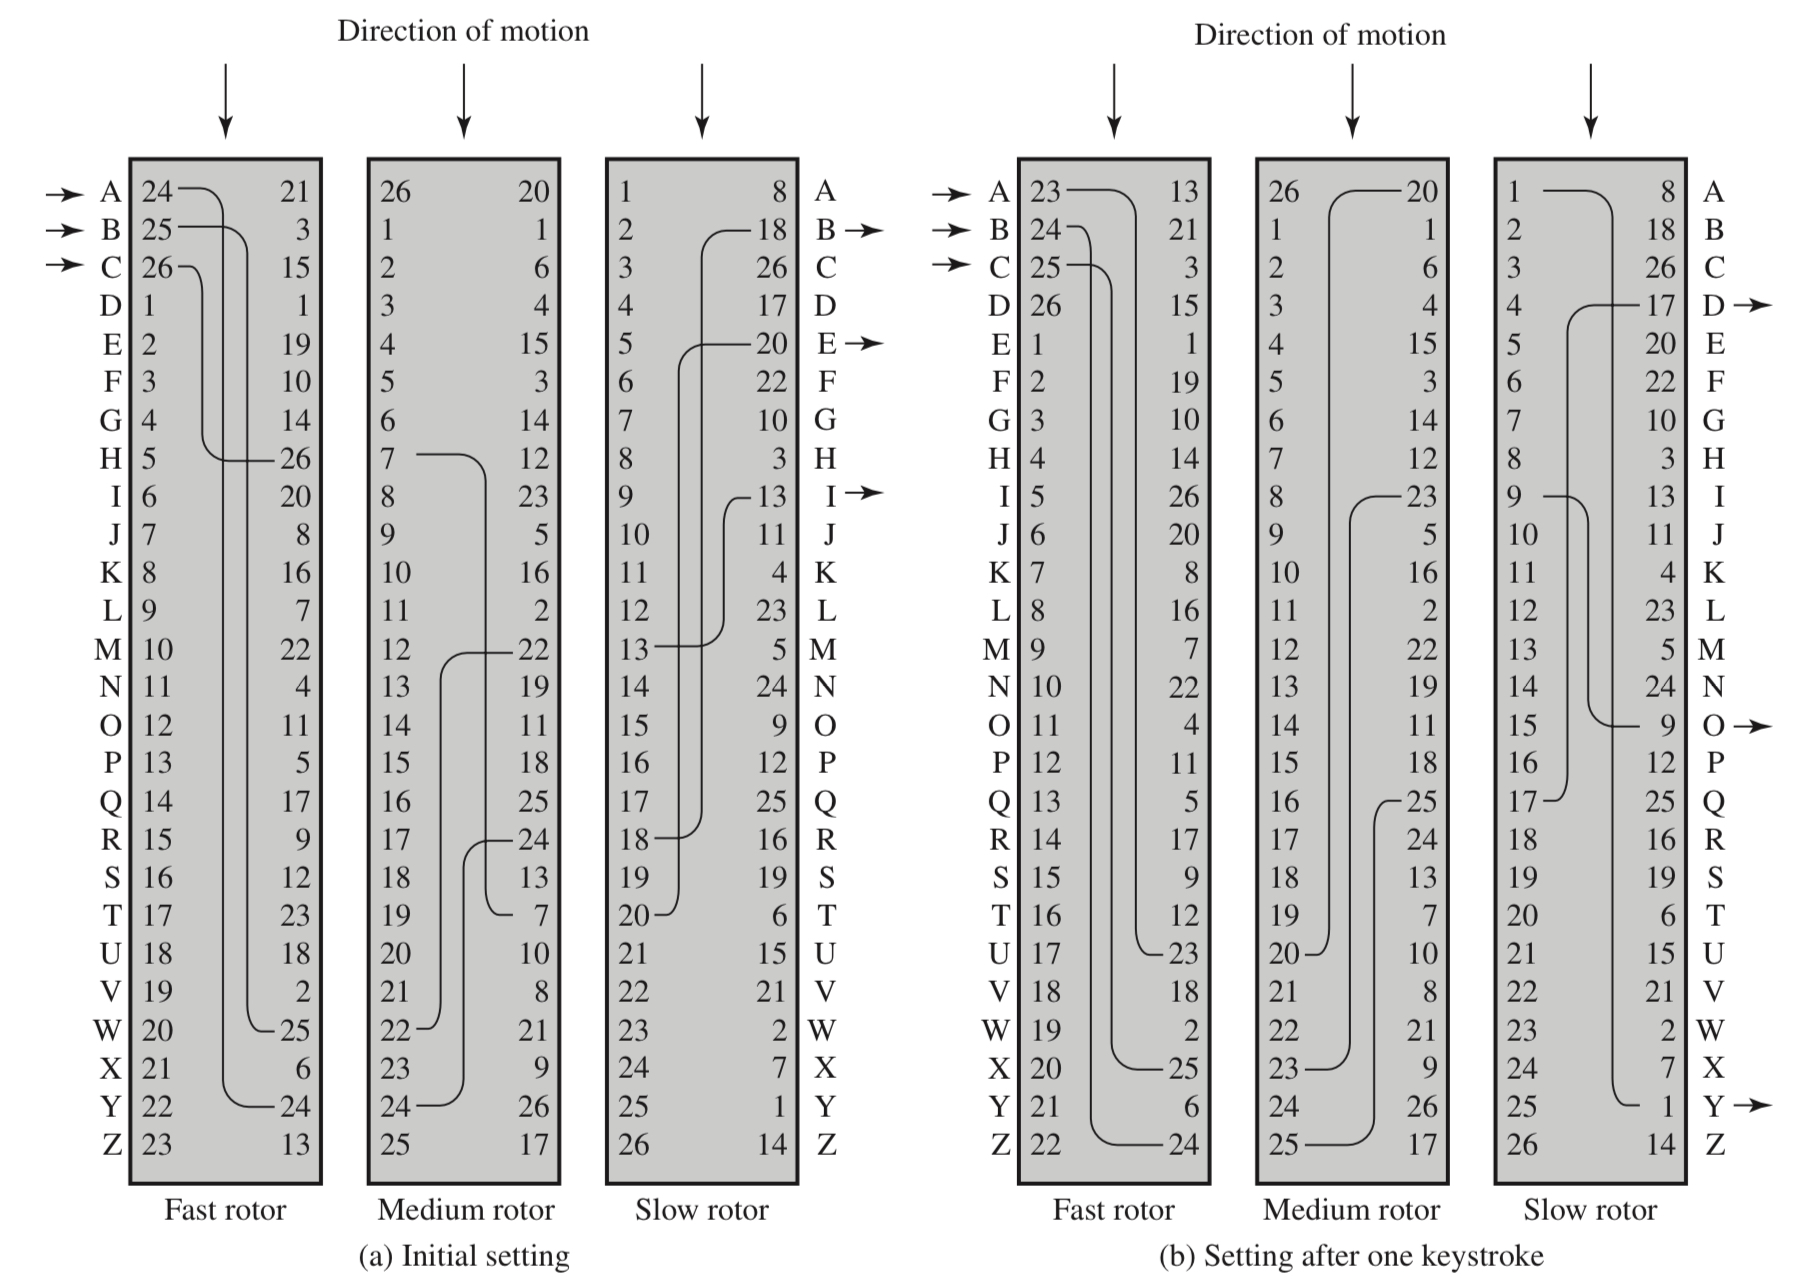
\includegraphics[width=0.8\textwidth]{img/Concatenazione_crittosistemi.png}
    \caption{Macchina a rotori}
\end{figure}

\subsubsection{Enigma}
La macchina Enigma è una macchina elettromeccanica portatile utilizzata per cifrare e decifrare
messaggi segreti. È stata utilizzata in Germania durante la seconda guerra mondiale.
La decodifica dei messaggi è molto complessa, vista la grande quantità di combinazioni possibili.

Se ho a una macchina che per essere decifrata ha bisogno di un tempo più alto della validità 
dei dati, allora posso dire che è sicura.

Il modo per decodificare i messaggi è stato fondamentale sapere che il messaggio iniziava con
una parola chiave, che era sempre la stessa. Sapendo questo, si poteva decodificare il messaggio
riducendo notevolmente l'insieme delle chiavi disponibili per la decodifica.
Conoscevano quindi il \textbf{plaintext}.

La concatenzione di crittosistemi è molto sicura, ma non è sicura contro gli attacchi
dove si conosce il plaintext.

\section{Classificazione dei livelli di sicurezza}
La classificazione si basa sulla difficoltà di violare il sistema, quindi sul tipo di 
attacchi a cui resiste.
\begin{itemize}
    \item \textbf{Known Cipher Text Attack}: l'attaccante conosce il testo cifrato.
    \item \textbf{Known Plaintext Attack}: l'attaccante vede il testo in chiaro e il corrispondente testo cifrato.
    \item \textbf{Chosen Plaintext Attack}: l'attaccante sceglie il testo in chiaro e conosce il corrispondente testo cifrato.
    \item \textbf{Adaptive Chosen Ciphertext Attack}: l'attaccante può continuamente scegliere il testo in chiaro e vedere il corrispondente testo cifrato.
\end{itemize}
La classifica è in base alla potenza che gli do nell'attaccarmi.
L'obiettivo è costruire un sistema che sia sicuro contro 
gli attacchi Adaptive Chosen Ciphertext Attack.
\section{Cifrari a flusso e a blocchi}
Un \textbf{cifrario a flusso} crittografa un flusso di dati digitali un bit
o un byte alla volta. Esempi di cifrari a flusso classici sono il
cifrario di Vigenère con autochiave e il cifrario di Vernam. Nell'ideale,
si utilizzerebbe una versione del cifrario di Vernam con one-time pad, in
cui lo stream di chiavi ha la stessa lunghezza dello stream di bit in chiaro.
Tuttavia, perché questo sia praticamente realizzabile, lo stream di chiavi deve
essere fornito in anticipo ad entrambi gli utenti attraverso un canale indipendente
e sicuro, il che può rappresentare una sfida logistica se il traffico dati
previsto è di grandi dimensioni.

Di conseguenza, per ragioni pratiche, il generatore di stream di bit deve
essere implementato come una procedura algoritmica, in modo che lo stream di
bit crittografico possa essere prodotto da entrambi gli utenti. In questo
approccio, il generatore di stream di bit è un algoritmo controllato dalla chiave
e deve produrre uno stream di bit crittograficamente robusto. I due utenti devono
condividere solo la chiave di generazione, e ognuno può generare lo stream di chiavi.

Un \textbf{cifrario a blocchi} tratta un blocco di testo in chiaro come un'entità
unica e produce un blocco di testo cifrato della stessa lunghezza. Di solito,
si utilizza una dimensione di blocco di $64$ o $128$ bit. Allo stesso modo del 
cifrario a flusso, i due utenti condividono una chiave di crittografia simmetrica.
Utilizzando alcune delle modalità di funzionamento spiegate in precedenza, un
cifrario a blocchi può essere usato per ottenere lo stesso effetto di un cifrario
a flusso.

Molto più sforzo è stato dedicato all'analisi dei cifrari a blocchi, poiché
sembrano essere applicabili a una gamma più ampia di applicazioni rispetto ai
cifrari a flusso. La maggior parte delle applicazioni crittografiche simmetriche
basate su rete fa uso di cifrari a blocchi. Pertanto, le discussioni in questo
contesto si concentreranno principalmente su di essi.

\subsection{Electronic Code Book}
Il ``Electronic Code Book" (\verb|ECB|) è una
delle modalità di funzionamento di un cifrario a blocchi, utilizzato per
crittografare un blocco di testo di lunghezza fissa. In questa modalità,
ogni blocco di testo in chiaro viene crittografato separatamente utilizzando
la stessa chiave. Non c'è alcuna dipendenza tra i blocchi di testo in chiaro
durante il processo di crittografia. Pertanto, gli stessi blocchi di testo in
chiaro generano gli stessi blocchi di testo cifrato. Tuttavia, questo comporta
il rischio di sicurezza in quanto pattern di testo in chiaro simili generano
pattern di testo cifrato simili, rendendo il sistema vulnerabile a un'analisi
statistica. Nonostante questa debolezza, l'\verb|ECB| è ancora utilizzato in alcuni
scenari in cui la semplicità e la velocità sono prioritarie rispetto alla
sicurezza, come per la crittografia di dati non sensibili o per applicazioni
specifiche in cui la perdita di alcuni blocchi non compromette la sicurezza
complessiva del sistema.

La modalità più semplice è la modalità di codifica elettronica (\verb|ECB|), in cui
il testo in chiaro viene gestito un blocco alla volta e ogni blocco di testo
in chiaro viene crittografato utilizzando la stessa chiave. Il termine ``codice"
è utilizzato perché, per una data chiave, esiste un testo cifrato univoco per
ogni blocco di testo in chiaro di b bit. Pertanto, possiamo immaginare un'enorme
tabella di corrispondenza in cui vi è una voce per ogni possibile modello
di testo in chiaro di $b$ bit che mostra il relativo testo cifrato corrispondente.
\begin{figure}[H]
    \centering
    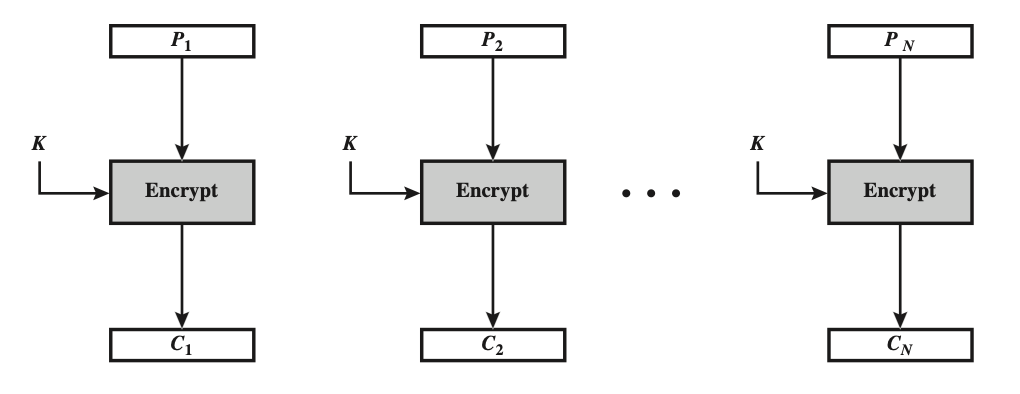
\includegraphics[width=0.5\textwidth]{img/electriccodeblock.png}
    \caption{Electronic Code Book}
\end{figure}

\subsection{Cipher Block Chaining}

La modalità di funzionamento ``Cipher Block Chaining'' (\verb|CBC|) è un metodo
di crittografia a blocchi che introduce un certo grado di indipendenza tra i
blocchi di testo in chiaro durante il processo di crittografia. Funziona come
segue:

\begin{enumerate}
    \item Prima di crittografare, viene generato un vettore di inizializzazione
    casuale noto come vettore di inizializzazione (\texttt{IV}). Questo vettore
    è combinato con il primo blocco di testo in chiaro tramite un'operazione di
    \texttt{XOR}.
    
    \item Il risultato di questa operazione \texttt{XOR} viene quindi
    crittografato utilizzando l'algoritmo di cifratura a blocchi insieme
    alla chiave.
    
    \item Il blocco di testo cifrato risultante viene poi combinato con il
    blocco di testo successivo prima della crittografia. Questo collegamento
    tra i blocchi di testo in chiaro aiuta a rompere la correlazione tra i
    blocchi di testo in chiaro, migliorando la sicurezza rispetto alla modalità
    di Electronic Code Book (\texttt{ECB}).
    
    \item Questo processo continua per tutti i blocchi di testo in chiaro
    successivi, garantendo che ciascun blocco di testo cifrato dipenda dal
    blocco di testo in chiaro precedente, oltre che dalla chiave.
\end{enumerate}

La decodifica avviene seguendo lo stesso processo in ordine inverso,
utilizzando il vettore di inizializzazione e la chiave per ottenere il
testo in chiaro originale.

La modalità \texttt{CBC} è considerata più sicura dell'\texttt{ECB} poiché
introduce una
dipendenza tra i blocchi di testo in chiaro, rendendo più complessa l'analisi
statistica e aumentando la resistenza agli attacchi crittoanalitici.
Tuttavia, è importante gestire correttamente il vettore di inizializzazione
per garantire la sicurezza e l'integrità del sistema di crittografia.
\[ C_j = E(K, [C_{j-1} \oplus P_j]) \]
\begin{figure}[H]
    \centering
    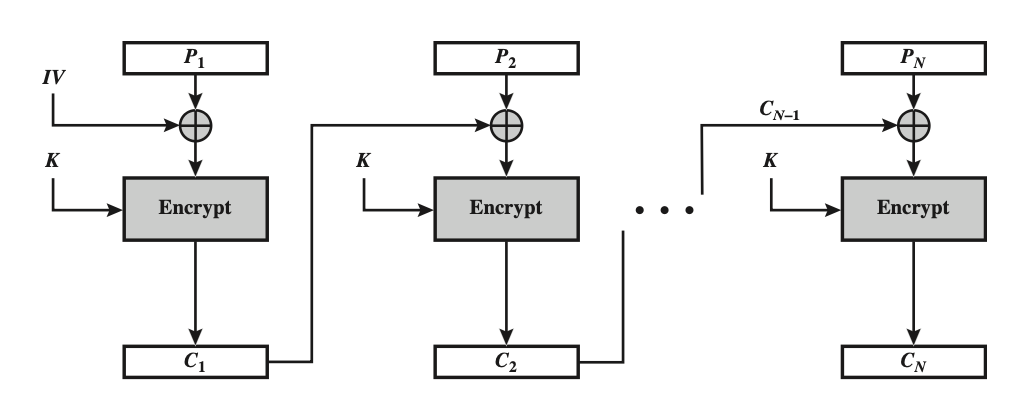
\includegraphics[width=0.8\textwidth]{img/CBC.png}
    \caption{Cipher Block Chaining}
\end{figure}
\subsection{Cipher Feedback}
Per \verb|AES|, \verb|DES| o qualsiasi altro cifrario a blocchi, la crittografia viene eseguita
su un blocco di \(b\) bit. Nel caso di \verb|DES|, \(b = 64\), e nel caso di \verb|AES|,
\(b = 128\). Tuttavia, è possibile convertire un cifrario a blocchi in un cifrario
a flusso utilizzando una delle modalità di funzionamento: la modalità di
Feedback di Cifratura (\verb|CFB|) e la modalità di Feedback di Output (\verb|OFB|).

Un cifrario a flusso elimina la necessità di aggiungere padding a un messaggio
per renderlo un numero intero di blocchi. Inoltre, può funzionare in tempo reale.
Pertanto, se viene trasmesso uno stream di caratteri, ogni carattere può essere
cifrato e trasmesso immediatamente utilizzando un cifrario a flusso orientato
ai caratteri.

Una proprietà desiderabile di un cifrario a flusso è che il testo cifrato abbia
la stessa lunghezza del testo in chiaro. Pertanto, se vengono trasmessi caratteri
di $8$ bit, ogni carattere dovrebbe essere cifrato per produrre un output di
testo cifrato di $8$ bit. Se vengono prodotti più di $8$ bit, la capacità di
trasmissione viene sprecata.

La modalità \verb|CFB| è illustrata nello schema. In questa modalità, il testo in chiaro
è diviso in segmenti di \(s\) bit, dove \(s\) è la dimensione dell'unità di
trasmissione. Durante la crittografia, viene utilizzato un registro a scorrimento
di \(b\) bit inizializzato con un vettore di inizializzazione (\verb|IV|). I
primi \(s\) bit più significativi dell'output della funzione di crittografia
vengono combinati con il primo segmento di testo in chiaro \(P_1\) tramite
l'operazione \texttt{XOR} per produrre l'unità di testo cifrato \(C_1\), che viene quindi
trasmessa. Il contenuto del registro a scorrimento viene spostato a sinistra di
\(s\) bit e \(C_1\) viene inserito nei \(s\) bit meno significativi del registro
a scorrimento. Questo processo continua fino a quando tutti i segmenti di testo
in chiaro sono stati crittografati.

Per la decodifica, viene utilizzato lo stesso schema, ad eccezione che l'unità
di testo cifrato ricevuta viene combinata tramite \verb|XOR| con l'output della funzione
di crittografia per produrre l'unità di testo in chiaro. È importante notare che
viene utilizzata la funzione di crittografia e non quella di decodifica. Questo
è facilmente spiegabile. Sia \(\texttt{MSBs}(X)\) definita come i \(s\) bit più significativi
di \(X\). Quindi

\[ C_1 = P_1 \oplus \texttt{MSBs}[E(K, IV)] \]

Di conseguenza, riarrangiando i termini:

\[ P_1 = C_1 \oplus \texttt{MSBs}[E(K, IV)] \]
\begin{figure}[H]
    \centering
    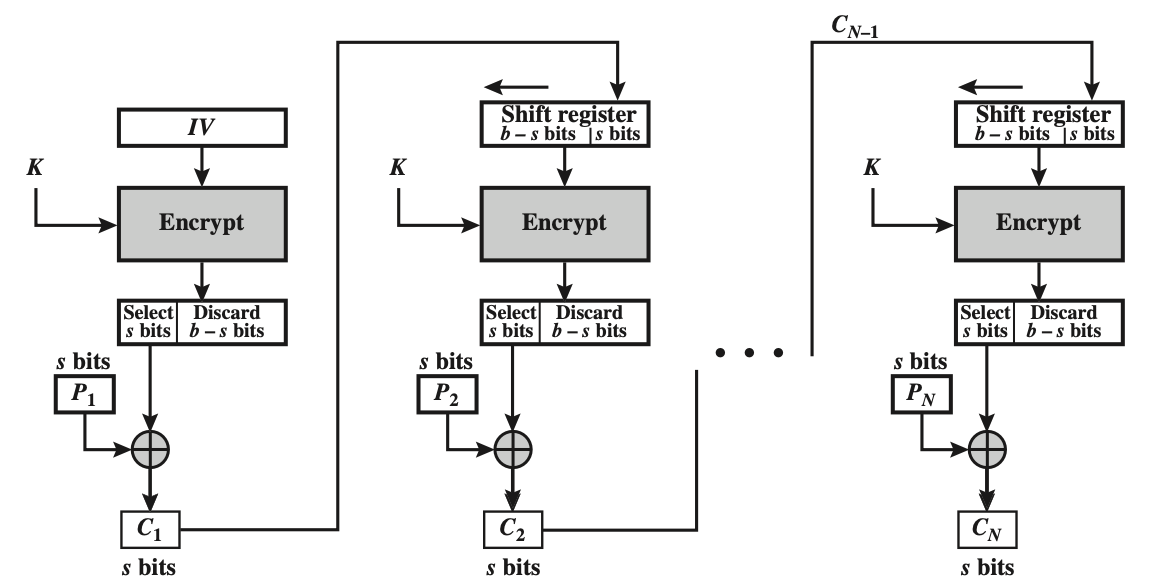
\includegraphics[width=0.8\textwidth]{img/cipherFeedback.png}
    \caption{Cipher Feedback}
\end{figure}
\subsection{Output Feedback}
La modalità di Feedback di Output (\verb|OFB|) ha una struttura simile a
quella di \verb|CFB|. Per \verb|OFB|, l'output della funzione di crittografia viene
retroalimentato e diventa l'input per crittografare il blocco successivo
di testo in chiaro. In \verb|CFB|, l'output dell'unità \verb|XOR| viene
retroalimentato e diventa l'input per crittografare il blocco successivo.
L'altra differenza è che la modalità \verb|OFB| opera su blocchi completi
di testo
in chiaro e testo cifrato, mentre \verb|CFB| opera su un sottoinsieme di \(s\) bit.
La crittografia \verb|OFB| può essere espressa come:

\[ C_j = P_j \oplus E(K, O_{j-1}) \]
\[ O_{j-1} = E(K, O_{j-2}) \]

Un po' di riflessione dovrebbe convincerti che possiamo riscrivere
l'espressione di crittografia come:

\[ C_j = P_j \oplus E(K, [C_{j-1} \oplus P_{j-1}]) \]

Riarrangiando i termini, possiamo dimostrare che la decodifica funziona:

\[ P_j = C_j \oplus E(K, [C_{j-1} \oplus P_{j-1}]) \]

\begin{figure}[H]
    \centering
    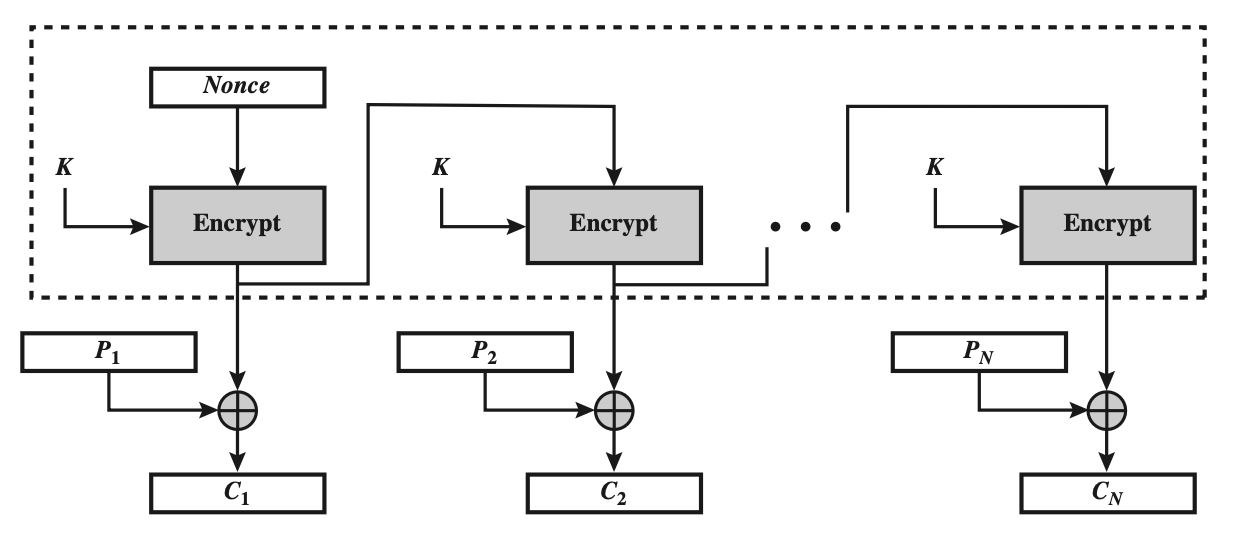
\includegraphics[width=0.8\textwidth]{img/outputFeedback.png}
    \caption{Output Feedback}
    \label{fig:outputFeedback}
\end{figure}
I blocchi di output della cifratura, \(O_i\), dipendono solo dalla chiave
e dal vettore di inizializzazione (\verb|IV|) e non dipendono dal testo
in chiaro. Pertanto, per una data chiave e \verb|IV|, lo stream di bit di
output utilizzato per l'operazione \texttt{XOR} con lo stream di bit in chiaro è fisso.
Se due messaggi diversi avessero un blocco identico di testo in chiaro
nella stessa posizione, un attaccante sarebbe in grado di determinare
quella parte dello stream \(O_i\).

Un vantaggio del metodo \verb|OFB| è che gli errori di bit nella trasmissione non
si propagano. Ad esempio, se si verifica un errore di bit in \(C_1\), solo
il valore ripristinato di \(P_1\) viene influenzato; i blocchi di testo in
chiaro successivi non vengono corrotti. Con \verb|CFB|, \(C_1\) serve anche come
input al registro a scorrimento e quindi causa corruzioni aggiuntive a valle.

Lo svantaggio di \verb|OFB| è che è più vulnerabile a un attacco di modifica dello
stream di messaggi rispetto a \verb|CFB|. Considera che complementare un bit nel
testo cifrato complementa il bit corrispondente nel testo in chiaro
ripristinato. Pertanto, possono essere effettuate modifiche controllate
al testo in chiaro ripristinato. Questo potrebbe rendere possibile per un
avversario, apportando le modifiche necessarie alla parte di checksum del
messaggio e alla parte di dati, modificare il testo cifrato in modo che non
sia rilevato da un codice di correzione degli errori.

\verb|OFB| ha la struttura di un tipico cifrario a flusso, poiché il cifrario
genera uno stream di bit come funzione di un valore iniziale e di una chiave,
e questo stream di bit viene operato con \verb|XOR| con i bit del testo in chiaro.
Lo stream generato che viene operato con \verb|XOR| con il testo in chiaro è
indipendente dal testo in chiaro stesso; questo è evidenziato da riquadri
tratteggiati in Figura (\ref{fig:outputFeedback}). Una differenza rispetto
ai cifrari a flusso è che \verb|OFB| crittografa il testo in chiaro un blocco
intero alla volta, dove tipicamente un blocco è di $64$ o $128$ bit. Molti
cifrari a flusso crittografano un byte alla volta.

\section{Rete di Feistel}
Moltissimi algoritmo di cifratura a blocchi utilizzano tale struttura.
La struttura di Feistel è una struttura di rete iterativa che è stata
progettata per essere utilizzata in cifrari a blocchi.
Tale struttura ha delle caratteristiche distintive:
\begin{itemize}
    \item L'input viene diviso in due metà.
    \item Esegue molteplici \textit{round} di cifratura, dove in ogni round 
    le due metà vengono elaborate in modo come segue:
    \begin{itemize}
        \item La metà sinistra diventa la metà destra del round precedente.
        \[
          L_i = R_{i-1}  
        \]
        \item La metà destra diventa l'applicazione della funzione di \texttt{XOR}
        tra la metà sinistra del round precedente e l'output della funzione $f$ che prende 
        in input la metà destra del round precedente e la chiave del round precedente.
        \[
            R_i = L_{i-1} \oplus f(R_{i-1}, K_{i-1})
        \]
    \end{itemize}
    \item La struttura è simmetrica, il che significa che la decodifica 
    avviene semplicemente invertendo l'ordine delle chiavi usate per la cifratura.
    \begin{itemize}
        \item \[ R_{i-1} = L_i \]
        \item \[L_{i-1} = R_i \oplus f(L_i, K_i)\]
    \end{itemize}
\end{itemize}
Il vantaggio è che le funzioni $f$ usate sono \textbf{one-way}.
\begin{tcolorbox}[title=One-way function]
    Una funzione $f: \{0,1\}^* \rightarrow \{0,1\}^*$ è \textbf{one-way} se esiste un algoritmo 
    che in tempo polinomiale mappa $x$ in $f(x)$ per ogni $x \in \{0,1\}^*$ e per ogni algoritmo 
    probabilistico polinomiale $\mathcal{A}$, ogni polinomio $p(\cdot)$
    e ogni intero $n$ sufficientemente grande, si ha che la probabilità che $\mathcal{A}$
    trovi un $x$ tale che $f(\mathcal{A}(f(x))) = f(x)$ è minore di $1/p(n)$.
\end{tcolorbox}
Anche se un algoritmo ha accesso a un metodo efficiente per generare valori che, una volta
processati dalla funzione $f$, producono un output, è estremamente improbabile che tale algoritmo 
possa invertire la funzione e trovare l'input originale dato l'output, almeno senza una 
quantità impraticabile di tempo e risorse.
\begin{figure}[H]
    \centering
    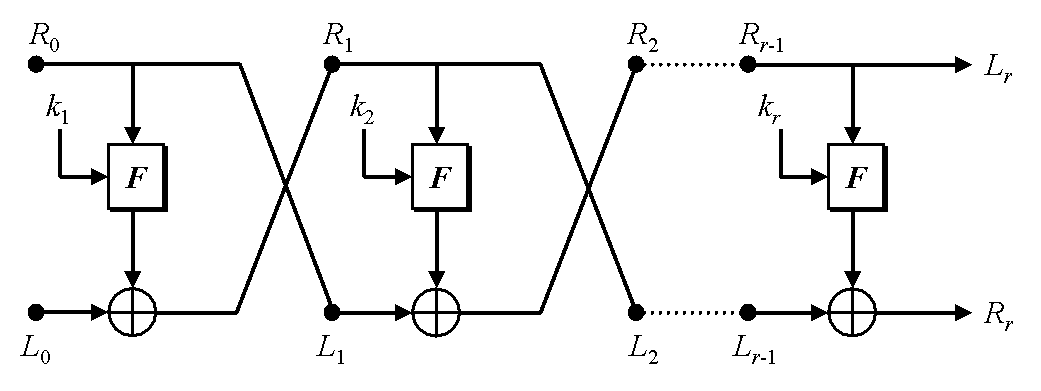
\includegraphics[width=0.8\textwidth]{img/feistel.png}
    \caption{Rete di Feistel}
\end{figure}
\section{Data Encryption Standard - \texttt{DES}}
\texttt{DES} è un cifrario a blocchi a chiave simmetrica che utilizza una struttura di Feistel.

La chiave è di $56$ bit, ma in realtà sono $64$ bit, di cui $8$ sono di parità, ed 
opera su blocchi di $64$ bit. 
L'algoritmo esegue una permutazione iniziale dei bit del blocco di testo in chiaro,
nota come \textit{Initial Permutation (IP)}, che riordina i bit secondo uno schema
fisso predefinito. Questo è seguito da 16 round di cifratura che consistono in espansione,
mescolamento con una chiave di round derivata dalla chiave principale, sostituzione tramite S-Box
e una permutazione finale. La funzione di round prende input dalla metà destra del blocco di dati
e la chiave di round, producendo un output che è poi combinato con la metà sinistra attraverso
un'operazione XOR.

Dopo l'ultimo round, le due metà del blocco vengono scambiate, e questo è seguito da una
\textit{Final Permutation (FP)}, che è l'inverso della permutazione iniziale. Il risultato
è il blocco di testo cifrato. La decodifica con \texttt{DES} segue lo stesso processo ma
in ordine inverso, utilizzando le chiavi di round in ordine inverso.

Nonostante la sua ampiamente testata sicurezza, la principale vulnerabilità di \texttt{DES}
risiede nella lunghezza della chiave. Tecniche come l'attacco a forza bruta, che era
teoricamente possibile ma non praticabile al tempo della sua creazione, sono divenute
fattibili con l'avanzamento della potenza di calcolo. Per questo motivo, \texttt{DES}
è stato sostituito da \texttt{AES} come standard approvato dal NIST (\textit{National
Institute of Standards and Technology}) per la cifratura di informazioni sensibili.
\subsection{Funzione di round}
La funzione di round prende in input $32$ bit e una chiave di round di $48$ bit e produce
un output di $32$ bit. La funzione di round è composta da quattro passaggi:
\begin{enumerate}
    \item \textbf{Espansione}: i $32$ bit di input vengono espansi a $48$ bit tramite una
    permutazione fissa.
    \item \textbf{Mescolamento}: i $48$ bit vengono combinati con la chiave di round tramite
    un'operazione di \texttt{XOR}.
    \item \textbf{Sostituzione}: Dopo il mescolamento con la chiave di round, i $48$ bit vengono
    passano attraverso $8$ \texttt{S-BOX}, ciascuno dei quali sostituisce $6$ bit con $4$ bit. 
    Sono lineari e complesse per aggiungere sicurezza alla cifratura.
    \item \textbf{Permutazione}: i $32$ bit vengono permutati tramite una permutazione fissa.
\end{enumerate}
L'alternanza di sostituzioni mediante \texttt{S-BOX}, permutazioni mediante permutazioni fisse
e espansioni forniscono la \textbf{confusione} e la \textbf{diffusione}, concetti introdotti
da \texttt{Shannon} e che sono alla base di molti cifrari moderni.

\begin{tcolorbox}[title=Confusione]
    Si tratta della relazione tra il testo in chiaro e la chiave. Deve essere difficile
    dedurre la chiave a partire dal testo cifrato. Ogni bit del testo cifrato deve
    dipendere da molti bit della chiave.
\end{tcolorbox}

\begin{tcolorbox}[title=Diffusione]
    Si tratta della capacità di un algoritmo di distribuire le correlazioni statistiche
    del testo lungo tutto l'alfabeto utilizzato dall'algoritmo di cifratura, rendendo quanto 
    più difficile un attacco statistico.
\end{tcolorbox}
\chapter{Teoria dei numeri}
\section{Proprietà dei numeri}

La teoria dei numeri è una branca fondamentale della matematica che studia le proprietà degli interi e delle loro relazioni. Nel contesto della teoria dei numeri, diversi concetti chiave emergono dall'analisi delle operazioni e degli insiemi numerici.

\begin{tcolorbox}[title={Operazioni chiuse}]
Un'operazione si dice chiusa se l'operazione applicata a due numeri naturali restituisce un numero naturale.
\[
  \mathbb{N} \, \texttt{op} \, \mathbb{N} \to \mathbb{N}  
\]
Ad esempio, l'addizione e la moltiplicazione sono operazioni chiuse sugli interi.
\end{tcolorbox}

Quando un'operazione non è chiusa? La divisione, non produce sempre un numero naturale. Gli insiemi sono inoltre caratterizzati da proprietà che li rendono unici.

\begin{tcolorbox}[title={Proprietà commutativa}]
  \[
    a \, \texttt{op} \, b = b \, \texttt{op} \, a
  \]
L'addizione e la moltiplicazione sono esempi di operazioni che soddisfano la proprietà commutativa.
\end{tcolorbox}

\begin{tcolorbox}[title={Proprietà associativa}]
  \[
    \forall a, b, c \in A \qquad a \, \texttt{op} \, (b \, \texttt{op} \, c) = (a \, \texttt{op} \, b) \, \texttt{op} \, c
  \]
La proprietà associativa è verificata dall'addizione e dalla moltiplicazione su diversi insiemi numerici.
\end{tcolorbox}

\begin{tcolorbox}[title={Elemento neutro}]
  \[
    a \, \texttt{op} \, e = a
  \]
  quindi 
  \[
    \exists e \in A \texttt{ t.c. }\forall a \in A \, a \, \texttt{op} \, e = e \, \texttt{op} \, a = a
  \]
L'elemento neutro per l'addizione è lo zero, mentre per la moltiplicazione è l'unità.
\end{tcolorbox}

\begin{tcolorbox}[title={Elemento inverso}]
  \[
    \forall a \in A \, \exists a^{-1} \in A \texttt{ t.c. } a \, \texttt{op} \, a^{-1} = a^{-1} \, \texttt{op} \, a = e
  \]
Alcuni esempi di elementi inversi includono l'opposto di un numero per l'addizione e il reciproco di un numero non nullo per la moltiplicazione.
\end{tcolorbox}

Ogni volta che definiamo delle strutture matematiche che soddisfano tali proprietà, si parla di gruppi. Un \textbf{gruppo} è
una struttura algebrica che rispetta determinate regole, tra cui chiusura, associatività, presenza di un elemento neutro e di un elemento inverso.

Prendiamo in considerazione i numeri naturali rispetto all'operazione di somma. Hanno l'inverso? No, quindi non è un gruppo. Tuttavia,
se aggiungessimo altri elementi e arrivassimo ai numeri interi, allora avremmo un gruppo rispetto alla somma. Allo stesso modo, se
considerassimo i numeri interi rispetto alla moltiplicazione (\textit{senza lo zero}), non avremmo l'inverso. In questo caso, dovremmo aggiungere
gli inversi e arrivare ai numeri razionali, che costituiscono un gruppo rispetto alla moltiplicazione.

Capita spesso di avere strutture che non sono gruppi. In questi casi, si possono seguire due approcci: ridurre la struttura eliminando
gli elementi che non soddisfano le proprietà del gruppo o espandere la struttura aggiungendo elementi in modo da soddisfare tali proprietà.

Vorremmo lavorare su un'algebra diversa, possibilmente con gruppi finiti. In particolare, ci concentreremo su gruppi che costituiscono
l'algebra alla base dei nostri algoritmi crittografici. Utilizzeremo funzioni che sono facili da calcolare ma difficili da invertire,
comunemente conosciute come \textbf{one-way function}. Queste funzioni si basano sull'algebra moltiplicativa.

Successivamente, esamineremo anche la crittografia ellittica, che si basa su un'algebra diversa, operando su curve ellittiche. Tuttavia,
gli algoritmi fondamentali rimarranno gli stessi, utilizzando però un'algebra additiva.

\section{Classe di equivalenza $\mathbb{Z}_n$}
Possiamo dire che:
\[
  \mathbb{Z}_n \equiv \mathbb{Z}_n \qquad a \equiv b \pmod{n} \iff (a \mod n) = (b \mod n)
\]
Quindi due numeri sono equivalenti se hanno lo stesso resto nella divisione per $n$.
Ad esempio, $5 \equiv 11 \pmod{3}$, perché entrambi hanno resto 2 nella divisione per 3.

Quando abbiamo una relazione di equivalenza possiamo costruire l'insieme degli oggetti equivalenti tra loro. 
L'insieme degli insiemi di oggetti equivalenti forma una \textbf{partizione}, gli elementi di tale 
partizione sono detti \textbf{classi di equivalenza} e si denotano mediante parentesi quadre di un elemento di tale classe.
Ogni singola classe di equivalenza può essere rappresentata da un qualsiasi elemento della classe stessa. 
\[
  \mathbb{Z}_n = \{0,1,2,3,\dots, n-1\}
\]

Un'analogia può essere fatta con le ore. Se sono le 10:00, allora sono anche le 22:00,
perché entrambe sono equivalenti a 10:00 $\pmod{12}$, o con le frazioni. È l'insieme 
delle classi di equivalenza tra numeri naturali dove due coppie sono 
equivalenti se hanno lo stesso prodotto incrociato, quindi il prodotto 
dei medi è uguale al prodotto degli estremi. Ad esempio, $2 \times 3 = 1 \times 6$. 
\[
  \frac{1}{2} \equiv \frac{3}{6}
\]
La rappresentazione canonica di una classe di equivalenza in $\mathbb{Z}_n$ è il suo
rappresentante minimo, ovvero un numero naturale compreso tra 0 e $n-1$.

Su tale insieme voglio definire delle operazioni.
\subsection{Somma}
La somma di due classi di equivalenza è definita come la classe di
equivalenza della somma dei rappresentanti. Ad esempio, se voglio
calcolare $[2] + [3]$, allora calcolo $2 + 3 = 5$ e la classe di equivalenza
di 5 è $[5]$. In generale, la somma di due classi di equivalenza è la classe
di equivalenza della somma dei rappresentanti.
\[
  [a] + [b] \stackrel{\Delta}{=} [a + b]
\]
Tale rappresentazione è buona solo se il risultato è indipendente dagli elementi 
delle due classi originali.
\subsubsection{Proprietà}
\begin{itemize}
  \item \textbf{Commutativa}: $\forall a, b \,[a] + [b] = [b] + [a]$.
  \item \textbf{Associativa}: $\forall a, b, c \,[a] + ([b] + [c]) = ([a] + [b]) + [c]$.
  \item \textbf{Elemento neutro}: $\exists e \in \mathbb{Z}_n \, \forall a \, [a] + [a] = [a] + [a] = [a]\qquad e = 0$.
  \item \textbf{Elemento inverso}: $\forall a \, \exists a^{-1} \in \mathbb{Z}_n \,
  \text{t.c.} \, [a] + [a^{-1}] = [a^{-1}] + [a] = [e] \qquad a^{-1} = -a$.
\end{itemize}
L'insieme $\mathbb{Z}_n$ con l'operazione di somma forma un \textbf{gruppo abeliano}, (
\textit{abeliano} perché commutativo).
\subsection{Moltiplicazione}
La moltiplicazione di due classi di equivalenza è definita come la classe di
equivalenza del prodotto dei rappresentanti. Ad esempio, se voglio
calcolare $[2] \cdot [3]$, allora calcolo $2 \cdot 3 = 6$ e la classe di equivalenza
di 6 è $[6]$. In generale, la moltiplicazione di due classi di equivalenza è la classe
di equivalenza del prodotto dei rappresentanti.
\[
  [a] \cdot [b] \stackrel{\Delta}{=} [a \cdot b]
\]
Tale rappresentazione è buona solo se il risultato è indipendente dagli elementi
delle due classi originali.
\subsubsection{Proprietà}
\begin{itemize}
  \item \textbf{Commutativa}: $\forall a, b \,[a] \cdot [b] = [b] \cdot [a]$.
  \item \textbf{Associativa}: $\forall a, b, c \,[a] \cdot ([b] \cdot [c]) = ([a] \cdot [b]) \cdot [c]$.
  \item \textbf{Elemento neutro}: $\exists e \in \mathbb{Z}_n \, \forall a \, [a] \cdot [a] = [a] \cdot [a] = [a]\qquad e = 1$.
\end{itemize}
L'insieme $\mathbb{Z}_n$ con l'operazione di moltiplicazione forma un \textbf{semigruppo}, 
ovvero un gruppo senza l'elemento inverso.
Per ottenere un gruppo, devo aggiungere l'elemento inverso. Per ottenere tale elemento,
quindi passare da un semigruppo ad un gruppo, 
posso seguire diverse strade; arricchire l'insieme con nuovi elementi, oppure
eliminare elementi.

Consideriamo l'insieme $\mathbb{Z}_n - \{0\}$ con l'operazione di moltiplicazione e consideriamo 
un esempio con $n = 15$.
\[
  \mathbb{Z}_{15} - \{0\} = \{1,2,3,4,5,6,7,8,9,10,11,12,13,14\}
\]
\begin{itemize}
  \item L'inverso moltiplicativo di $1$ è $1$.
  \item L'inverso moltiplicativo di $2$ è $8$ ($2 \cdot 8 = 16 \equiv 1 \pmod{15}$).
  \item L'inverso moltiplicativo di $3$ non c'è.
  \item \dots
\end{itemize}
Notiamo che non tutti gli elementi hanno un inverso moltiplicativo, quindi non 
posso costruire un gruppo. Per ottenere un gruppo, devo eliminare gli elementi
che non hanno un inverso moltiplicativo.
L'insieme $\mathbb{Z}_{15} - \{0, 3, 5, 6, 9, 10, 12\}$ che sarà quindi:
\[
  \mathbb{Z}_{15}^* = \{1,2,4,7,8,11,13,14\}
\]
Abbiamo quindi definito l'insieme $\mathbb{Z}_n^*$:
\[
  \mathbb{Z}_n^* = \{a \in \mathbb{Z}_n \, | \, \texttt{mcd}(a, n) = 1\}
\]
Ovvero l'insieme dei numeri che sono relativi primi con $n$.
Moltiplicando due numeri relativamente primi con $n$, ottengo un numero
relativamente primo con $n$. L'operazione di moltiplicazione è chiusa in $\mathbb{Z}_n^*$.
\begin{theorem}[Teorema di Eulero]
  Per ogni $a, b \, \exists x,y \, ax + by = \texttt{mcd}(a,b)$
\end{theorem}
Se $a \in \mathbb{Z}_n^*$ allora $\texttt{mcd}(a, n) = 1$ per definizione e quindi
\[
  ax + ny = 1
\] 
\[
  ax = 1 - ny
\]
\[
  ax \equiv 1 \pmod{n}
\]
Quindi la classe di equivalenza di $x$ è l'inverso moltiplicativo di $a$.
La necessità di lavorare con gruppi nasce dal fatto che in informatica
è necessario lavorare con insiemi finiti, in questo caso algebre su insiemi 
finiti, in particolare sui gruppi, in modo da manipolare gli elementi in 
base alle proprietà.
\section{Gruppi e generatori}
Sia $\mathcal{G}$ un gruppo, un operatore $\otimes$. Sia $g$ un elemento di $\mathcal{G}$.
\[
  g = g^1 \qquad g \otimes g = g^2 \qquad g \otimes g \otimes g = g^3 \qquad \dots \qquad g \otimes g 
  \otimes g \otimes \dots \otimes g = g^n
\]
Continuando a moltiplicare $g$ per se stesso, non arriverò ad un qualsiasi $n$ generico, poiché 
il gruppo è finito. Quindi, supponiamo  che arrivi a $g \otimes g 
\otimes g \otimes \dots \otimes g = g^{\lvert \mathcal{G} \rvert}$ e che l'esponente successivo 
sia $g^{\lvert \mathcal{G} \rvert + 1}$. Per il \textbf{pumping lemma} avrò sicuramente 
almeno un elemento ripetuto.
\begin{theorem}
  Per ogni gruppo $\mathcal{G}$ finito, per ogni $a \in \mathcal{G}$, 
  \[
    a^{\lvert \mathcal{G} \rvert} = 1
  \]
\end{theorem}
Da questo teorema segue che se sicuramente $a^{\lvert \mathcal{G} \rvert} = 1$ ovvero l'elemento neutro,
ma per un gruppo $\mathcal{G}$ finito, potrei avere anche che per un qualche
$a^i = 1$.

Se prendo tutte le potenze di $g$ ottengo un sottogruppo dell'insieme $\mathcal{G}$, un sottogruppo 
continua ad essere un gruppo. Se quello che ottengo è un sottogruppo proprio, ovvero 
un sottogruppo che non è tutto l'insieme $\mathcal{G}$, allora $G$ è ciclico e $g$ è un 
\textbf{generatore} di $\mathcal{G}$.
\begin{theorem}
  Sia $\mathcal{G}'$ è sottogruppo di $\mathcal{G}$, allora $\lvert \mathcal{G}' \rvert \mid
  \lvert \mathcal{G} \rvert$.
\end{theorem}
\subsubsection{Esempio}
\[
  \mathbb{Z}_{15}^* = \{1,2,4,7,8,11,13,14\}
\]
\begin{itemize}
  \item $1$
  \item $2 \cdot 2 = 4 \cdot 2 = 8 \cdot 2 = 16$ quindi $2^4 \equiv 1 \pmod{15}$
  \item $4 \cdot 4 = 16 \equiv 1 \pmod{15}$
  \item $7 \cdot 7 = 49 \equiv 4, 4 \cdot 7 = 28 \equiv 13, 13 \cdot 7 = 91 \equiv 1 \pmod{15}$
  \item $8 \cdot 8 = 64 \equiv 4, 4 \cdot 8 = 32 \equiv 2, 2 \cdot 8 = 16 \equiv 1 \pmod{15}$
  \item $11 \cdot 11 = 121 \equiv 1 \pmod{15}$
  \item $13 \cdot 13 = 169 \equiv 4, 4 \cdot 13 = 52 \equiv 7, 7 \cdot 13 = 91 \equiv 1 \pmod{15}$
  \item $14 \cdot 14 = 196 \equiv 1 \pmod{15}$
\end{itemize}
La cardinalità di $\mathbb{Z}_{15}^*$ è $8$, ma questo gruppo non è ciclico, poiché non esiste un
elemento generatore che generi tutto il gruppo.
\subsection{Generatori primi}
Se prendo $\mathbb{Z}_{n}^*$ con $n$ primo, allora $\mathbb{Z}_{n}^*$ è ciclico, poiché
ogni elemento di $\mathbb{Z}_{n}^*$ è un generatore di $\mathbb{Z}_{n}^*$.
In generale un numero primo non può essere scomposto in fattori, quindi:
\[
  \mathbb{Z}_{p}^* = \{1,2,3,\dots,p-1\}
\]
\subsubsection{Esempio}
\[
  \mathbb{Z}_{7}^* = \{1,2,3,4,5,6\}
\]
\begin{itemize}
  \item $1$
  \item $2 \cdot 2 = 4 \cdot 2 = 8 \equiv 1 \pmod{7}$
  \item $3 \cdot 3 = 9 \equiv 2, 2 \cdot 3 = 6, 6 \cdot 3 = 18 \equiv 4, 4 \cdot 3 = 12 \equiv 5, 5 \cdot 3 = 15 \equiv 1 \pmod{7}$
  \item $4 \cdot 4 = 16 \equiv 2, 2 \cdot 4 = 8 \equiv 1 \pmod{7}$
  \item $5 \cdot 5 = 25 \equiv 4, 4 \cdot 5 = 20 \equiv 6, 6 \cdot 5 = 30 \equiv 2, 2 \cdot 5 = 10 \equiv 3, 3 \cdot 5 = 15 \equiv 1 \pmod{7}$
  \item $6 \cdot 6 = 36 \equiv 1 \pmod{7}$
\end{itemize}
Abbiamo che $\mathbb{Z}_{7}^*$ è ciclico, poiché esiste un generatore che genera tutto il gruppo, in questo 
caso $3$ e $5$.

\subsection{Probabilità dei numeri primi}
\begin{theorem}[Densità dei numeri primi]
  La densità dei numeri primi è proporzionale al numero di bit che compongono il numero.
\end{theorem}
Suppongo di avere un numero casuale $n$ di $k$ bit, allora la probabilità che $n$ sia primo è 
$\frac{1}{k}$. Supponiamo di voler comporre un numero $n$ di $k$ bit, utilizzo un algoritmo
che mi generi tale numero. 

Per verificare che tale numero sia primo, utilizzo una algoritmo casuale 
che sceglie casualmente un numero $a$ tra $1$ e $n-1$ e verifica che il numero 
scelto sia primo. Statisticamente circa la metà dei numeri scelti sono testimoni del fatto 
che un numero non sia primo. Se il test fallisce e mi dice che il numero non è primo, allora
termino. Se il test ha esito positivo allora scelgo un altro numero $a$ e ripeto il test di 
primalità.
Se tutte le volte che scelgo un numero $a$ il test ha esito positivo, allora la probabilità 
di accettare la primalità di $n$ è $\frac{1}{2^t}$, dove $t$ è il numero di volte che ho
ripetuto il test (\textit{eventi indipendenti}), abbassando la probabilità di errore notevolmente.

Sulla base di questo ragionamento, siamo in grado di generare numeri primi molto grandi.
\chapter{Crittografia a chiave pubblica}
\section{Crittografia a chiave pubblica}
L'idea di crittografia a chiave pubblica è quella di avere due chiavi, una
pubblica $P_k$ e una privata $S_k$. La chiave pubblica è nota a tutti, mentre
quella privata è nota solo al proprietario. 
Con codifica avviene con la chiave pubblica, mentre la decodifica avviene con la
chiave privata.

Ovviamente l'idea di fondo è avendo in mano il testo cifrato non si riesce a
risalire al testo in chiaro senza la chiave privata. Chiunque può cifrare un
messaggio, ma solo il proprietario della chiave privata può decifrarlo.

In un sistema a chiave pubblica abbiamo i seguenti algoritmi:
\begin{itemize}
    \item Un algoritmo di generazione delle chiavi:
    \[
        \mathcal{G}: 1^k \to (P_k, S_k) 
    \]
    Dove $1^k$ è un parametro che indica la lunghezza della chiave, ovvero il \textit{security parameter}.
    \item Un algoritmo di encription:
      \[
        \mathcal{E}: m, P_k \to \mathcal{E}(m, P_k)
    \]
    \item Un algoritmo di decription:
    \[
          \mathcal{D}: C, S_k \to D(C, P_k)
    \]
\end{itemize}
Ovviamente vale la seguente relazione:
\begin{equation}
    \forall m \quad \mathcal{D}(\mathcal{E}(m, P_k), S_k) = m
\end{equation}
Oltre al fatto che decriptare un messaggio a partire dal testo cifrato senza 
la chiave privata è computazionalmente intrattabile. L'idea è che più la chiave
è lunga più è difficile rompere il sistema. L'idea è che il security parameter
$k$ è proporzionale alla lunghezza della chiave e al crescere di $k$ cresce
la sicurezza del sistema.

Gli algoritmi citati sono algoritmi probabilistici polinomiali. Se voglio 
affermare che tali algoritmi sono polinomiali l'input che rappresenta la 
lunghezza della chiave non può essere 
rappresentato in binario, perché la lunghezza della chiave sarebbe
esponenziale nel numero di bit utilizzati per rappresentare il numero. 
Sulle macchine di Turing la dimensione del problema è data dal numero di 
celle del nastro di input. Utilizzando la teoria della complessità 
basata su tali macchine, o in ogni caso su sistemi dove la dimensione 
dell'input è lo spazio che occupa nella nostra rappresentazione. Per 
voler dire che un algoritmo è polinomiale nel \textbf{valore del 
security parameter} e non nel modo in cui è rappresentato, imponiamo 
che il security parameter sia rappresentato in \textbf{unario}, ovvero 
tanti uni quanti la lunghezza della chiave.

\section{Diffie-Hellman}
Il problema di Diffie-Hellman è il seguente: Alice e Bob vogliono
scambiarsi un segreto senza che Eve lo possa intercettare. Lo strumento 
utilizzato per risolvere il problema è del logaritmo discreto.

Si fissa a priori un numero primo $p$ e un generatore $g$ di $\mathbb{Z}_p^*$.
Un agente A sceglie un numero $x \in_R \{1, \dots, p-1\}$ e calcola $g^x \mod p$. 
Un agente B sceglie un numero $y \in_R \{1, \dots, p-1\}$ e calcola $g^y \mod p$.

\begin{figure}[H]
    \centering
    \begin{tabular}[H]{l|l|l}
        & \textbf{Public} & \textbf{Private} \\
        \hline
        A & $g^x \mod p$ & $x$ \\
        \hline
        B & $g^y \mod p$ & $y$ \\
    \end{tabular}
\end{figure}

A questo punto A e B possono calcolare $g^{xy} \mod p$ e $g^{yx} \mod p$, che coincidono.

Il sistema è sicuro perché calcolare $g^{xy} \mod p$ è computazionalmente intrattabile. Avendo 
a disposizione $g^x$ e $g^y$ non è possibile calcolare $g^{xy}$. Se sappiamo rispondere al problema 
del logaritmo discreto, allora possiamo risolvere il problema di Diffie-Hellman, tale algoritmo 
potrebbe esistere, ma non è stato ancora trovato.

Sia $\mathcal{A} \in \texttt{PPT}$ che calcola $g^{xy} \mod p$ a partire da $g^x \mod p$ e $g^y \mod p$. 
Usiamo $\mathcal{A}$ per costruire un algoritmo $\mathcal{B}$ che risolve il problema del logaritmo discreto,
ma tale dimostrazione non è ancora stata data, perciò non l'algoritmo di Diffie-Hellman non è dimostrabilmente 
sicuro. non siamo in grado di dire che rompere Diffie-Hellman è almeno difficile quanto risolvere il problema
del logaritmo discreto.

\subsection{Ipotesi di Diffie-Hellman}
Qualcuno potrebbe costruire un algoritmo che si basa sull'ipotesi che l'algoritmo di Diffie-Hellman sia sicuro.
\begin{tcolorbox}[title = Ipotesi di Diffie-Hellman]
    Siano $x, y, z$ dei numeri causali scelti in $\{1, \dots, p-1\}$, allora è difficile 
    distinguere ($g^x, g^y, g^{xy}$) da ($g^x, g^y, g^z$).
\end{tcolorbox}

Il concetto di distinguibilità è un concetto probabilistico, ovvero che la possibilità di poter 
distinguere due insiemi di elementi è trascurabile. Ovvero che la probabilità di distinguere 
sia inferiore a $1/2 + \epsilon$, dove $\epsilon$ è trascurabile. Quindi l'attaccante non abbia 
alcun vantaggio rispetto ad un attaccante che non ha alcuna informazione.
Se un attaccante avesse anche un minimo vantaggio, allora potrebbe utilizzare tale vantaggio per
ottenere informazioni sul segreto. Tale vantaggio può essere utilizzato per ottenere l'informazione 
totale mediante esperimenti ripetuti.

\section{Rivest Shamir Adleman - RSA}
$g^x$ è una funzione che è facile da calcolare, ma è difficile da invertire, ovvero calcolare $x$
a partire da $g^x$. Una funzione con questa proprietà è detta \textbf{one-way function}. Il protocollo di 
Diffie-Hellman è sicuro se e solo se esiste una one-way function.
Vorremmo che la one-way function sia anche \textbf{trapdoor}, ovvero che esista un algoritmo 
efficiente che permetta di invertire la funzione. Tale algoritmo è detto \textbf{trapdoor algorithm}.
La trapdoor è una informazione aggiuntiva che permette di invertire la funzione.

Siano $p, q$ due numeri primi molto grandi, $n = pq$. Sia $e$ un numero casuale tale che 
\texttt{mcd}(e, $\varphi(n)$) = 1, dove $\varphi(n) = (p-1)(q-1)$, ovvero il numero di Eulero. Scegliamo 
une elemento $d$ co-primo con $\varphi(n)$ tale che $de \equiv 1 \mod \varphi(n)$.
La chiave pubblica è la coppia $(n, e)$, mentre la chiave privata è la coppia $(n, d)$.
\subsubsection{Algoritmo di cifratura}
\[
  \mathcal{E}: m, (n, e) \mapsto m^e \mod n  
\]
\subsubsection{Algoritmo di decifratura}
\[
  \mathcal{D}: c, (n, d) \mapsto c^d \mod n
\]
\subsection{Funzionamento}
Proviamo a prendere un messaggio $m$ e a cifrarlo con la chiave pubblica $(n, e)$,
e proviamo a decodificarlo con la chiave privata $(n, d)$.
\[
  (m^e)^d = m^{ed} = m^{k\varphi(n) + 1} = m \cdot (m^{\varphi(n)})^k \equiv m \mod n  
\]
Infatti $d\cdot e$ è congruo a 1 modulo $\varphi(n)$, quindi $d\cdot e = k\varphi(n) + 1$.
Per il teorema del resto cinese, $m^{k\varphi(n) + 1} \equiv m$, e non solo per gli elementi 
di $\mathbb{Z}_n^*$.

La funzione one way è la funzione di codifica, quindi $m^e$, l'inversa di 
$m^e$ è la radice $e$-esima, ovvero $m = c^{1/e}$, ma per calcolare la radice $e$-esima
ad oggi non esiste un algoritmo efficiente. L'unico modo per calcolare la radice $e$-esima
è calcolare $d$ e decifrare il messaggio, quindi $d$ è l'informazione trapdoor.

Ci piacerebbe dimostrare che se fossimo in grado di invertire la radice 
e-esima di un numero allora saremmo in grado di fattorizzare $n$, o di calcolare 
il residuo quadratico. Se fosse vero, allora RSA sarebbe sicuro, ma non è stato ancora
dimostrato ad oggi. L'unica sicurezza di RSA è l'esistenza dell'ipotesi di RSA.
\subsection{Attacchi a RSA}
Ci sono casi in cui RSA è stato attaccato, il motivo però era legato alla cattiva 
implementazione dell'algoritmo, e non all'algoritmo in sé.
Quando parliamo di un crittosistema in realtà parliamo di un insieme di algoritmi,
e non di un singolo algoritmo. L'algoritmo di generazione delle chiave impone 
la scelta \textbf{casuale} di $e$ in modo uniforme con gli elementi 
primi con $\varphi(n)$, ma se non fosse casuale, allora potremmo avere dei problemi.
\subsubsection{Attacco sulla base di messaggi piccoli}
Inoltre, in caso di messaggi piccoli, quindi se $m^e < n$, vuol dire che 
non applico nemmeno l'operazione di modulo, e vuol dire in particolare che 
la radice $e$-esima di $m^e$ è una normale radice $e$-esima nell'aritmetica 
dei numeri interi, e quindi è facile da calcolare.
Lavorando con messaggi che a livello numerico sono piccoli, allora 
invertiamo tutto facilmente, più è piccola $e$, più è facile avere 
messaggi che elevati a $e$ sono più piccoli di $n$. Bisogna quindi
star attenti a scenari in cui $m^e < n$.
\subsubsection{Attacco sulla base di messaggi sparsi}
Altri problemi che potrebbe avere RSA sono legati allo spargimento dei 
messaggi.
Immaginiamo di avere un messaggio:

\begin{center}
  \texttt{Buongiorno, il suo voto è 30L}\\
  \texttt{Buongiorno, il suo voto è 30}\\
  \texttt{Buongiorno, il suo voto è 29}\\
  \dots\\
  \texttt{Buongiorno, il suo voto è 0}\\
\end{center}
Uno che vuole decifrare il messaggio può prendere i $32$ messaggi e
cifrarli tutti, per poi distinguerli.
Se con RSA devo codificare messaggi che sono presi da un insieme piccolo,
devo far attenzione perché potrei venir attaccato da qualcuno che utilizza 
la stessa chiave pubblica.
\subsubsection{Attacco sulla informazione parziale}
Siamo sicuri che tutti i bit di questa inversa siano difficili da calcolare?
Non è che sulla radice $e$-esima di $m^e$ ci sono dei bit che sono più facili 
da calcolare? Ai fini di dire che il sistema è sicuro, non è 
sufficiente dire che il cypertext non si sappia ricavare il plaintext,
vorremmo dire che dal cypertext non si riesca a ricavare nessuna informazione 
binaria sul plaintext. Ma come possiamo definire tale proprietà?
\subsubsection{Attacco sulla base di messaggi ripetuti}
Per difendersi da tale problema, aggiungo un po' di rumore al messaggio,
ovvero aggiungo un po' di bit casuali al messaggio, in modo tale che con 
alta probabilità il messaggio non sia mai uguale. In questo modo, anche se
il messaggio è sempre lo stesso, il cypertext è sempre diverso, utilizzando 
quindi la probabilistic encryption.
\section{Sicurezza di un crittosistema}
RSA è sicuro perché non conosciamo un algoritmo probabilistico polinomiale 
per calcolare la radice $e$-esima di un numero. Ma cosa vuol dire?
Se esistesse un algoritmo probabilistico polinomiale per calcolare la radice 
$e$-esima di un numero con probabilità $\frac{1}{k}$, sarebbe un problema,
perché reiterando l'algoritmo $k$ volte, avrei una probabilità di successo.

Se fossimo nello scenario in cui con un $a\in_R \mathbb{Z}_n^*$, l'algoritmo 
mi dia risposta corretta con probabilità $\frac{1}{k}$, potremmo dichiararci 
tranquilli? No, perché potrebbero attaccare sempre.

Fissando $a$ e scegliendo $r \in_R \mathbb{Z}_n^*$, calcolo $(a\cdot r)^e \mod n$,
se prendo un elemento casuale di $\mathbb{Z}_n^*$ e lo elevo ad $e$, ottengo
l'oggetto che è distribuito uniformemente in $\mathbb{Z}_n^*$. Sappiamo che
l'elevamento di $r$ alla $e$-esima è distribuito uniformemente in $\mathbb{Z}_n^*$, 
perché $e$ è stata scelta in maniera tale che la radice $e$-esima dia esattamente 
$r$. Quindi $r^e$ è una funzione invertibile, di conseguenza la funzione che mappa $r$ in 
$r^e$ è una funzione biettiva, quindi un elemento scelto uniformemente in $\mathbb{Z}_n^*$
viene mappato da $r^e$ in un elemento scelto uniformemente scelto in $\mathbb{Z}_n^*$.
Ogni volta che prendiamo un elemento e creiamo una suriezione dello stesso insieme, 
se l'elemento di partenza è scelto uniformemente, il risultato della suriezione, che nella 
sostanza è una permutazione, è scelto uniformemente.

Se prendiamo $r^e$ e lo moltiplichiamo per $a$, otteniamo un elemento che è distribuito
uniformemente in $\mathbb{Z}_n^*$, perché $a$ è scelto uniformemente in $\mathbb{Z}_n^*$, 
poiché la moltiplicazione per $a$ è una funzione biettiva, perché $a$ ammette inverso.

Siamo partiti da un elemento fissato e abbiamo costruito un elemento distribuito uniformemente
e causale, se a quell'elemento applichiamo l'algoritmo della radice $e$-esima, otteniamo
$\frac{1}{k}$ di probabilità di successo, ma se ripetiamo l'algoritmo $k$ volte, abbiamo
una probabilità di successo di $1$, rendendo quindi l'algoritmo indipendente dalla $a$ di 
partenza.
\[
  ar^e \rightarrow \sqrt[e]{ar^e} = r \sqrt[e]{a}
\]
Quindi se prendo il risultato e lo divido per $r$, ottengo $\sqrt[e]{a}$,
che è distribuito uniformemente in $\mathbb{Z}_n^*$, perché $r$ è distribuito uniformemente.

Ed ecco che abbiamo un algoritmo che a partire da una blackbox che con $a$ causale 
calcola correttamente la radice $e$-esima di $a$ una volta su $k$, abbiamo una macchina 
che con $a$ fissato calcola la radice $e$-esima di $a$ con probabilità $1$.

La macchina che calcola la radice $e$-esima di $a$ darà una sequenza di bit, che
potrebbe essere la radice $e$-esima di $a$, oppure no. Bisognerebbe riconoscere la risposta
corretta, rielevando il risultato ad $e$, se ottengo l'input allora la risposta è 
corretta, altrimenti no.

Quindi abbiamo trasformato un algoritmo che funziona una volta su $k$ in un algoritmo
che funziona in un tempo medio di $k$.
\begin{tcolorbox}[title=Definizione di sicurezza]
  Diciamo che un sistema è attaccabile se il tempo medio per attaccarlo è polinomiale.
\end{tcolorbox}
Se esistesse un qualsiasi algoritmo in grado di attaccare la radice $e$-esima di $a$,
con una probabilità polinomiale in $k$, riusciamo a costruire un algoritmo che calcola
la stessa cosa con un tempo medio polinomiale in $k$.

Visto che partiamo  dall'idea che non esista un algoritmo probabilistico polinomiale 
in grado di calcolare la radice $e$-esima di $a$, allora non esiste un algoritmo
che sia in grado di calcolarlo con una probabilità che sia polinomialmente piccola.
Quindi la \textbf{probabilità di successo è più piccola di qualsiasi polinomio}, dove per polinomio 
si intende:
\[
  \probP[\texttt{attacco}] < \frac{1}{k}\quad \forall c
\]
Fissando un polinomio, con chiavi corte, però, la possibilità di trovare un polinomio esiste, 
perciò bisogna correggere tale definizione.
\begin{equation}
  \forall c \exists \bar{k} \forall k > \bar{k}\quad\probP[\texttt{attacco}] < k^{-c}
\end{equation}
Per attacco non intendiamo solo il fatto di non poter essere in grado di poter calcolare la 
radice $e$-esima di $a$, ma anche il fatto di non essere in grado di capire 
\textbf{informazioni binarie}.

L'algoritmo che calcola la radice $e$-esima di $a$ è l'algoritmo che calcola la
la fattorizzazione di $n$, la fattorizzazione di $n$ è l'informazione 
binaria che vogliamo proteggere.textbf{trapdoor} che permette di risolvere 
il problema.
\begin{tcolorbox}[title=Fattorizzazione di $n$]
  Si pensa che non esista un algoritmo \texttt{PPT} che dati $n$, $e$ e $a$,
  calcola $\sqrt[e]{a} \in \mathbb{Z}_n^*$ con probabilità polinomiale.
\end{tcolorbox}
\subsection{Utilizzo pratico di RSA}
Nel caso pratico il costo computazionale di RSA è molto alto, infatti codificare 
un blocco di $k$ bit con RSA richiede $k$ esponenziazioni modulari, ovvero $k^3$, 
un costo computazionale molto alto. Per questo motivo RSA viene utilizzato per
codificare una chiave di sessione, che viene utilizzata per codificare
il messaggio con un algoritmo simmetrico, che è molto più veloce di RSA.
Tipicamente l'algoritmo utilizzato è l'algoritmo simmetrico \texttt{AES} (\ref{section:des}).

Tra l'altro vi è una notevole differenza con Diffie-Hellman, infatti in Diffie-Hellman
riesco a scambiarmi un'unica chiave, a meno che non faccia un nuovo scambio di chiavi,
ogni volta.

Se si parte dall'idea che la crittografia simmetrica sia meno sicura della crittografia
asimmetrica, allora si può pensare di utilizzare una chiave di sessione diversa dopo 
un certo periodo. Con RSA è possibile fare questo, perché è possibile scambiarsi
chiavi diverse, mentre con Diffie-Hellman non è possibile, perché si dovrebbero scambiare
chiavi diverse ogni volta, e questo è molto costoso. La generazione della chiave di sessione 
per Diffie-Hellman è molto costosa, per via delle Certification Authority, che devono
essere coinvolte nel processo di generazione della chiave di sessione per certificare 
le chiavi pubbliche.

\section{Crittosistema di Micali per la codifica di un singolo bit}
\subsubsection{Algoritmo di generazione delle chiavi}
Si sceglie un numero primo $p_1$ e un numero $p_2$ tale che moltiplicati tra loro
diano un numero $n$ tale che $n = p_1p_2$. I due numeri devono essere scelti in modo
casuale con $\frac{k}{2}$ bit ciascuno, dove $k$ è la lunghezza della chiave. Sia 
$y \in_R$ ai non quadrati con simbolo di Jacobi $1$ modulo $n$. Ricordiamo che per 
costruire un numero non quadrato causale con simbolo di Jacobi $1$ basta scegliere un numero
casuale e verificare che il simbolo di Jacobi sia $1$, ovvero che appartenga 
a $\mathbb{Z}_n^*$, se non lo è si sceglie un altro
numero casuale e si ripete il procedimento. A questo punto verifico che il simbolo 
di Legendre rispetto a $p_1$ e $q_1$ sia $-1$. 

La chiave pubblica è:
\[
  P_k = (n, y)
\]
La chiave privata è:
\[
  S_k = (p_1, p_2)
\]
L'ipotesi di base è che sia difficile fattorizzare $n$, ma il problema di 
riferimento sarà il problema del residuo quadratico, ovvero il problema di
calcolare la radice quadrata di un numero modulo $n$.
\subsubsection{Algoritmo di codifica}
L'algoritmo di codifica prende un bit $b$, sia $x \in_R \mathbb{Z}_n^*$, se 
$b$ è $0$ allora $c = x^2 \mod n$, altrimenti $c = xy^2 \mod n$. 
$x^2$ è un quadrato casuale di $\mathbb{Z}_n^*$, mentre $xy^2$ è un 
non quadrato con simbolo di Jacobi $1$. Se prendo un quadrato con simbolo di 
Jacobi $1$ e lo moltiplico per un non quadrato con simbolo di Jacobi $1$ ottengo
un non quadrato con simbolo di Jacobi $1$. Se il quadrato è casuale, allora 
ottengo un non quadrato casuale con simbolo di Jacobi $1$ distribuito uniformemente
tra tutti i non quadrati con simbolo di Jacobi $1$.

Il risultato è che la codifica di $0$ è un quadrato a caso, mentre la codifica di $1$ è
un non quadrato a caso con simbolo di Jacobi $1$.
\[
  \mathcal{E}: \{0, 1\} \to x \in_R \mathbb{Z}_n^*
\]
\[
  f(x) = \begin{cases}
    x^2 \mod n & \text{se } b = 0\\
    xy^2 \mod n & \text{se } b = 1
  \end{cases}
\]
\subsubsection{Algoritmo di decodifica}
L'algoritmo di verifica prende in input $c$ e verifica se $c$ è un quadrato 
rispetto a $p_1$ e $p_2$, ovvero se $c$ è un residuo quadratico modulo $p_1$ e
modulo $p_2$. Se $c$ è un quadrato rispetto a $p_1$ e $p_2$ allora $b = 0$,
se entrambe le verifiche falliscono allora $b = 1$, in altri casi non siamo in presenza 
di un cypertext valido.
\[
  \left(\frac{c}{p_1}\right) = \left(\frac{c}{p_2}\right) = 1 \qquad \text{allora } b = 0
\]
\[
  \left(\frac{c}{p_1}\right) = \left(\frac{c}{p_2}\right) = -1 \qquad \text{allora } b = 1
\]
\subsection{Rompere il crittosistema di Micali}
Rompere tale protocollo significherebbe disporre di un algoritmo $\mathcal{A}$ che preso in 
input in cyphertext $c$ e la chiave pubblica $P_k$ restituisce $b$ con probabilità
diversa da $\frac{1}{2}$, poiché siamo in un contesto binario.

Un attaccante quindi dovrebbe essere in grado di ottenere un vantaggio rispetto 
a qualcuno che non conosce nulla, ovvero che indovini con probabilità $\frac{1}{2}$.
Il vantaggio consiste nell'allontanarsi da $\frac{1}{2}$, sia in positivo che in negativo, 
poiché se si allontana in negativo basta invertire il risultato per ottenere
un vantaggio positivo.

Il numero di esperimenti deve essere tale che la differenza delle probabilità sia
maggiore di $\frac{1}{2}$, ma il numero di esperimenti deve essere un numero 
polinomiale, in modo tale da poter osservare tali esperimenti in tempo polinomiale.
\begin{tcolorbox}[title = Sicurezza]
  \begin{equation}
    \forall c \, \exists \bar{k} \, \forall k \geq \bar{k} \quad \mid \probP[\texttt{Successo}] - \frac{1}{2} \mid  > k^{-c}
  \end{equation}
\end{tcolorbox}
Supponiamo che la probabilità di successo sia maggiore di $\frac{1}{2} + \epsilon$ e vorrei che la probabilità di successo sia quindi 
prossima a $1$. Per farlo eseguo due tipologie di esperimenti, il primo ripete l'esperimento $k$ volte e mediante l'algoritmo che 
ha a disposizione il vantaggio è $\frac{1}{2} + \epsilon$, mentre il secondo esperimento ripete l'esperimento $k$ volte e mediante
esperimenti casuali, ovvero senza l'algoritmo, ottiene un vantaggio di $\frac{1}{2}$. Ripetendo l'esperimento un numero abbastanza grande di 
volte si ottiene il risultato desiderato, poiché basterebbe visualizzare le due distribuzioni per vedere in cosa differiscono. L'algoritmo 
quindi indovina con probabilità $1$. Più $\epsilon$ è piccolo, più esperimenti sono necessari per ottenere il risultato desiderato. 
Servirebbe quindi stimare, dato un $\epsilon$ fissato, il numero di esperimenti necessari per ottenere il risultato desiderato.
\subsubsection{Limite di Chernoff} \label{limite_chernoff}
\begin{tcolorbox}[title = Limite di Chernoff]
  Siano $X_1, \dots, X_n$ variabili casuali e binarie indipendenti con probabilità 
  di successo $\probP[X_i = 1] > \frac{1}{2}$ e $\probP[X_i = 0] = 1 - \probP[X_i = 1]$.
  La probabilità che più della metà delle variabili casuali siano $1$ è:
  \[
    \mathcal{P} = \sum_{i = \frac{n}{2} + 1}^n \binom{n}{i} \probP[X_i = 1]^i \probP[X_i = 0]^{n - i}
  \]
  \[
    \mathcal{P} \geq 1 - e^{-2n\left(p - \frac{1}{2}\right)^2}
  \]
  Tale formula dice che la probabilità che più della metà degli eventi dia $1$ è 
  esponenzialmente vicina a $1$, dove l'eponenzialmente è in funzione di $n$.
  \[
    \probP[\texttt{errore}] = e^{-2 \epsilon n}
  \]
  Dove $\epsilon$ è il vantaggio.
\end{tcolorbox}
Supponiamo di volere $e^{-2 \epsilon n} < \frac{1}{2^k}$, quindi:
\[
  e^{-2c\epsilon^2 n} < 2^{-k}
\]
\[
  -2\epsilon^2 n < c' - k 
\]
\[
  n > \frac{c' - k}{2\epsilon^2}
\]
Se $\epsilon$ è polinomiale in $k$ allora $n$ è polinomiale in $k$.
Di conseguenza, se il vantaggio è polinomiale in qualche security parameter, allora
si riesce ad ottenere una quantità di errore nel security parameter che è
esponenzialmente piccola, scegliendo una quantità di esperimenti polinomiale in esso.

Un sistema è attaccato nel momento in cui esiste un algoritmo polinomiale in 
grado di romperlo.

Nel momento in cui $\epsilon$ è un $k^{-c}$, allora $n$ (\textit{dove $n$ è il numero di
esperimenti}) è polinomiale in $k$.

Visto che l'ipotesi di partenza è che non esistano algoritmi probabilistici polinomiali in grado
di rompere il sistema (\textit{vero}) e visto che abbiamo dimostrato che esiste tale algoritmo (\textit{falso}), allora
l'algoritmo di Micali è sicuro.
\subsubsection{Costruzione degli esperimenti indipendenti}

Una volta capito che la costruzione di $n$ esperimenti indipendenti funziona, bisogna 
capire come costruirli. Supponiamo che la probabilità di successo sia $\frac{1}{2} + \epsilon$ e
di disporre di un algoritmo $\mathcal{A}$ che prende in input un numero $z$ 
con $\left(\frac{z}{n}\right) = 1$, in output restituisce che $z$ è quadrato oppure no.

Per farlo si sceglie $r_1, \dots, r_n \in_R \mathbb{Z}_n^*$ e
si calcola $w_i = z \cdot r_i^2$. L'algoritmo quindi prende in input $w_i$ e restituisce
$b_i$.
\[
  b_i = \mathcal{A}(w_i)
\]

In sostanza si prende in input un numero (\textit{cyphertext}) e l'algoritmo lo moltiplica per una 
quadrato a caso, quindi l'algoritmo restituisce $1$ se il risultato è un quadrato casuale e $0$
altrimenti.

Tale algoritmo però ha un difetto, ovvero che se $z$ è un quadrato, allora $w_i$ è un quadrato
sempre, quindi l'algoritmo restituisce sempre $1$, se invece $z$ non è un quadrato, allora
$w_i$ è un quadrato con probabilità $\frac{1}{2} + \epsilon$.
\subsubsection{Costruzione di un controesempio}
Supponiamo che $\mathcal{A}$ dica correttamente che il $40\%$ dei numeri quadrati sono quadrati e 
che il $62\%$ dei non quadrati sono non quadrati. Sostanzialmente l'algoritmo $\mathcal{A}$
ha una probabilità di successo a seconda dell'input che gli viene dato. 
\[
  \probP[\mathcal{A}(\texttt{n})\texttt{ successo}] = \frac{1}{2} \cdot \frac{40}{100} + 
  \frac{1}{2} \cdot \frac{62}{100} = \frac{51}{100} = 51\%
\]
L'approccio di costruzione degli esperimenti indipendenti non è corretto, perché 
non fornisce all'algoritmo $\mathcal{A}$ un input secondo la misura di probabilità
che $\mathcal{A}$ si aspetta, quando diciamo che ha una certa probabilità di successo.
L'esperimento corretto avviene solamente quando ad $\mathcal{A}$ viene dato un input
un oggetto che sia distribuito uniformemente tra gli oggetti con simbolo di Jacobi $1$.
\subsubsection{Costruzione degli esperimenti indipendenti corretta}
L'idea di base è quella di lanciare una moneta per decidere se invertire o meno la 
quadraticità di $z$ in modo da ottenere un input che sia distribuito uniformemente.
Siano $r_1, \dots, r_n \in_R \mathbb{Z}_n^*$ e siano $s_1, \dots, s_n \in_R \{0,1\}$.
\[
  \forall i \quad w_i = 
  \begin{cases}
    z \cdot r_i^2 & \text{se } s_i = 0 \\
    y \cdot z \cdot r_i^2 & \text{se } s_i = 1
  \end{cases}
\]
Sia $b_i = \mathcal{A}(w_i)$. In questo modo lasciamo una moneta $s_i$ che decide se mantenere 
la quadraticità di $z$ oppure no. Quindi $z \cdot r_i^2$ è un oggetto a caso tra gli oggetti con stessa 
quadraticità di $z$, mentre $y \cdot z \cdot r_i^2$ è un oggetto a caso tra gli oggetti con quadraticità 
opposta di $z$, di conseguenza $w_i$ è un oggetto a caso distribuito
uniformemente tra gli oggetti con simbolo di Jacobi $1$.
In questo caso quindi $\mathcal{A}$ ha una probabilità di successo di $\frac{1}{2} + \epsilon$, ma 
$b_i$ è la risposta al problema trasformato, ma non è la stessa del problema originale.
\[
  \forall i \qquad b_i' = 
  \begin{cases}
    b_i & \text{se } s_i = 0 \\
    \bar{b_i} & \text{se } s_i = 1
  \end{cases}
\]
perché se $s_i = 1$ allora nell'input ho invertito la quadraticità di $z$, di conseguenza la risposta deve essere 
a sua volta invertita per avere una risposta corretta nei confronti di $z$.

Tale costruzione funziona, poiché è possibile passare dall'algoritmo $\mathcal{A}'$
all'algoritmo $\mathcal{A}$, semplicemente invertendo la risposta quando $s_i = 1$, ma non
sempre ciò è attuabile, perché non sempre è possibile invertire la risposta.

L'algoritmo che calcola il residuo quadratico prende in input $z$ e restituisce $1$ se $z$ è un quadrato
e $0$ altrimenti, ma a tale algoritmo abbiamo dato in input $y$, ovvero un non quadrato con simbolo di Jacobi
$1$. Ma siamo davvero capaci di costruire un algoritmo che calcola un non quadrato con simbolo di Jacobi $1$
senza usare la fattorizzazione di $n$? La risposta è no, perché se fosse possibile allora sarebbe possibile
fattorizzare $n$.
\begin{figure}[H]
  \centering
  \begin{tikzpicture}
    % rettangolo con due input e un output
    \node[draw, rectangle, minimum width=4cm, minimum height=3cm] (A) at (0,0) {$\mathcal{A}'$};
    \draw[->] (-5, 0.5) -- (-2, 0.5) node[midway, above] {$z$};
    \draw[->] (-3, -0.5) -- (-2, -0.5) node[midway, below] {$y$};
    \draw[->] (2, 0) -- (5, 0) node[midway, above] {$\{0,1\}$};
    \node[draw, rectangle, minimum width=8cm, minimum height=5cm] (B) at (0,0) {};
    \node (AS) at (-3.2, 2) {$\mathcal{A}''$};
  \end{tikzpicture}
\end{figure}
Sappiamo quindi che la macchina funziona correttamente dato $y$, ma non disponiamo di tale valore.
Perché non prendere un $y$ a caso e verificare se è un quadrato? 

Sia $x \in_R \mathbb{Z}_n^*$ e sia $s \in_R \{0,1\}$, allora 
\[
  w =
  \begin{cases}
    x^2 & \text{se } s = 0 \\
    y \cdot x^2 & \text{se } s = 1
  \end{cases}
\]
Sia $b$ la risposta da utilizzare per l'algoritmo. Se per puro caso però $y$ fosse un quadrato, non riuscirei 
a cambiare la quadraticità di $w$ nel caso $s = 1$. Quindi nel caso in cui $s$ fosse 
uguale a $1$ e $y$ fosse un quadrato, allora $w$ sarebbe un quadrato, quindi la risposta dell'algoritmo sarebbe
sempre sbagliata, poiché verrebbe complementata la risposta pensando che $w$ non sia un quadrato. In ogni caso 
però è possibile sorvolare tale problema, poiché basta vedere come si comporta statisticamente 
la macchina in presenza di non quadrati e di quadrati. Il comportamento della macchina è per forza diverso di fronte 
alle due situazioni, perché altrimenti non sarebbe capace di distinguere i due input.
\section{Distinguisher}
Codificare $b_1, \dots, b_l$ in $E(b_1), \dots, E(b_l)$ può essere fatto facendo si che dal testo cifrato non si risalga 
al testo in chiaro. Dimenticandoci del problema della malleabilità, vorremmo che dal cyphertext non si possa risalire
ad alcuna informazione binaria sul plaintext, ma dobbiamo capire cosa vuol dire non poter risalire ad alcuna informazione
binaria.
\begin{tcolorbox}[title = Distinguisher]
  Un \textbf{distinguisher} è un algoritmo binario $\mathcal{D} \in \texttt{PPT}$ che restituisce $0$ o $1$. Il distinguisher
  prende in input un evento che soddisfa o meno una certa proprietà e 
  un altro evento che soddisfa o meno la stessa proprietà. Il distinguisher deve essere in grado di distinguere
  se i due eventi si comportano in modo diverso o meno.
  Statisticamente il distinguisher verifica che i due eventi si comportino in modo polinomialmente diverso
  (\ref{limite_chernoff}), altrimenti tale differenza non sarebbe distinguibile.
\end{tcolorbox}
Sia $\probP_k^{\mathcal{D}, m}$ la probabilità che il distinguisher $\mathcal{D}$ restituisca $1$ su input, una codifica 
di $m$ quando il security parameter vale $k$. Un sistema di codifica nascone $m_1$ e $m_2$ a $\mathcal{D}$ quando:
\begin{equation}
  \forall c \, \exists \bar{k} \, \forall k \geq \bar{k} \qquad
  |\probP_k^{\mathcal{D}, m_1} - \probP_k^{\mathcal{D}, m_2}| < k^{-c}
\end{equation}
Ovvero:
\begin{equation}
  |\probP_k^{\mathcal{D}, m_1} - \probP_k^{\mathcal{D}, m_2}| < k^{-\omega(1)}
\end{equation}
$E$ nasconde informazioni a $\mathcal{D}$ se per ogni $m_1$ e $m_2$ $E$ nasconde $m_1$ e $m_2$ a $\mathcal{D}$. 
$E$ nasconde se per ogni $\mathcal{D} \in \texttt{PPT}$ $E$ nasconde $m_1$ e $m_2$ a $\mathcal{D}$.
\begin{proof}
  Supponiamo per assurdo che $\exists \mathcal{D} \in \texttt{PPT}$ tale che 
  \[
    \exists m_1, m_2, \,\forall \bar{k} \, \exists k \geq \bar{k} \qquad
    |\probP_k^{\mathcal{D}, m_1} - \probP_k^{\mathcal{D}, m_2}| \geq k^{-c}
  \]
   Allora $\mathcal{D}$ può distinguere su due messaggi $m_1$ e $m_2$ che differiscono di un solo bit.
   \begin{equation*}
    m_1 = \alpha^1 \alpha^2 \dots \alpha^l \qquad
    m_2 = \beta^1 \beta^2 \dots \beta^l 
   \end{equation*}

Definisco $\forall i \in \{0,\dots,l\} \,m(i) = \beta^1 \dots \beta^{i-1} \beta^i \alpha^{i+1} \dots \alpha^l$, 
ovvero una serie di bit intermedi per poter passare da $m_1$ a $m_2$ variando un solo bit per volta.
Quindi $m(0) = m_1$, $m(l) = m_2$, di conseguenza $\probP_k^{\mathcal{D}, m(i)} = \probP(i)$, ovvero la probabilità 
che il distinguisher restituisca $1$ se viene data in input una codifica del messaggio $m_i$.
  \[
    \probP(0) = \probP_k^{\mathcal{D}, m_1} \qquad \probP(l) = \probP_k^{\mathcal{D}, m_2}
  \]
Scopriamo quindi che l'ipotesi diventa:
\[
  k^{-c} \leq |\probP(0) - \probP(l)| = |\sum_{i=0}^{l - 1} \probP(i) - \probP(i+1)| 
  \leq \sum_{i=0}^{l - 1} |\probP(i) - \probP(i+1)|
\]
Poiché sappiamo che $\probP(0) - \probP(1) + \probP(1) - \probP(2) + \dots + \probP(l-1) - \probP(l) = \probP(0) - \probP(l)$. 
Quindi:
\[
  \sum_{i=0}^{l - 1} |\probP(i) - \probP(i+1)| \geq k^{-c}
\]
Avendo la somma di numeri che eccede un determinato valore allora so che esiste almeno un elemento che è maggiore o uguale 
della media.
\[
  \exists i \in \{0,\dots,l-1\}\qquad \textit{t.c.} \qquad |\probP(i) - \probP(i+1)| \geq \frac{k^{-c}}{l} \geq k^{-(c+1)} = k^{-c'}
\]
Abbiamo quindi trovato un polinomio $c'$ tale per cui il distinguisher è in grado di distinguere due messaggi che differiscono
di un solo bit.
I due messaggi $m_1$ e $m_2$ differiscono di un solo bit, quindi:
\begin{align*}
  \begin{array}{r c lllllllll}
  m(i) & = & \beta^1 &\dots &\beta^{i-1} & \beta^i &\textcolor{red}{\alpha^{i+1}} & \alpha^{i+2} &\dots &\alpha^l \\
  m(i+1) & = & \beta^1 &\dots &\beta^{i-1} & \beta^i &\textcolor{red}{\beta^{i+1}} & \alpha^{i+2} &\dots &\alpha^l \\
  \end{array}
\end{align*}
A questo punto supponiamo senza perdita di generalità che $\alpha^{i+1} = 0$ e $\beta^{i+1} = 1$. Sia $z$ un 
elemento di $\mathbb{Z}_n^*$ con $\left( \frac{z}{n} \right) = 1$, quindi $z$ potrebbe essere la codifica di uno 
$0$ o di un $1$.

Dato $z$ viene costruito $E(\beta_1)E(\beta_2)\dots E(\beta_i)zE(\alpha_{i+2})\dots E(\alpha_l)$ e viene lanciato 
l'algoritmo $\mathcal{D}$ sul risultato. La probabilità con cui $\mathcal{D}$ restituisce $1$ è \probP(i) se $z$
codifica $0$ e $\probP(i+1)$ se $z$ codifica $1$ se in input viene data la codifica di $m(i)$ secondo 
l'algoritmo per codificare il messaggio $m_i$, ovvero applicando $E$ a tutti i bit del messaggio.
Avendo però aggiunto $z$ in mezzo al messaggio non ho codificato secondo l'algoritmo che il distinguisher
si aspetta, quindi bisogna codificare il messaggio $m(i)$ in maniera corretta:
\[
  E(\beta_1)E(\beta_2)\dots E(\beta_i)\,\textcolor{red}{z \cdot x^2}\,E(\alpha_{i+2})\dots E(\alpha_l)\qquad \text{con } 
  x \in \mathbb{Z}_n^*
\]
A questo punto il distinguisher restituisce $1$ con probabilità $\probP(i)$ se $z$
codifica $0$ e $\probP(i+1)$ se $z$.

Chiamiamo $\mathcal{P}_0$ la probabilità che il distinguisher restituisca $0$ (\textit{quindi $\probP(i)$}) e 
$\mathcal{P}_1$ la probabilità che il distinguisher restituisca $1$ (\textit{ovvero $\probP(i+1)$}) se in input dato è costruito come sopra.

Se si riceve la codifica di un bit scelto a caso, con quale probabilità si riesce a distinguere se è $0$ o $1$?
Si utilizza il risultato del distinguisher $\mathcal{D}$ come tentativo.
\[
  \probP[\texttt{indovinare}] = \frac{1}{2} \cdot (1 - \mathcal{P}_0) + \frac{1}{2} \cdot \mathcal{P}_1 = 
  \frac{1}{2} + \frac{1}{2} \cdot (\mathcal{P}_1 - \mathcal{P}_0)
\]
Se sottraiamo $\frac{1}{2}$ otteniamo:
  \begin{align*}
    \probP[\texttt{non indovinare}] &= \frac{1}{2} + \frac{1}{2} \cdot (\mathcal{P}_1 -
  \mathcal{P}_0) - \frac{1}{2} \\
  &= \frac{1}{2} \cdot (\mathcal{P}_1 - \mathcal{P}_0) \\
  &= \frac{1}{2} \cdot |\probP(i) - \probP(i+1)| \\
  &\geq \frac{1}{2} \cdot k^{-c'}
  \end{align*}
L'algoritmo ha quindi un vantaggio di almeno $\frac{1}{2} \cdot k^{-c'}$, quindi tale algoritmo è 
un attaccante.
\end{proof}
\subsection{Distinguere e indovinare}
TODO
\section{Lancio della moneta}
Il sistema descritto in precedenza ha un problema, infatti sappiamo che 
la codifica di un singolo bit richiede una quantità molto alta di bit. Infatti 
implicherebbe un enorme spreco di banda, di risorse. Ci piacerebbe giungere 
ad uno scenario in cui un singolo bit viene codificato con un solo bit.

Per arrivare a questo punto impareremo a costruire numeri \textbf{pseudo-casuali
crittograficamente sicuri} da utilizzare come base per simulare un one-time pad, 
dove la chiave non è realmente casuale, ma è una chiave generata da noi, 
ma nessuno con potenza di calcolo polinomiale possa realmente notare la 
differenza.

Il lancio di monete in rete è un problema molto importante, infatti simulare 
un reale lancio di monete è molto difficile, in quanto non si può avere
la certezza che uno dei due agenti non stia mentendo.
Disponiamo dei due agenti $A$ e $B$ che vogliono simulare un
lancio di moneta e che comunicano attraverso un canale di comunicazione
e vorremmo che il lancio avvenga in modo simile a quello reale, ovvero
che entrambi gli agenti non sappiano il risultato del lancio prima che
questo avvenga e che il risultato sia frutto del lancio di una moneta.

Il fatto che $A$ lanci la moneta e che comunichi il risultato a $B$ non
va bene, poiché il risultato può essere manipolato da $A$ affinché sia 
di suo gradimento, e l'altro agente non può avere la certezza che il
risultato sia reale.
Si potrebbe provare a comunicare il risultato in contemporanea, ma anche
in questo caso si potrebbe simulare un ritardo di rete in modo da 
sfruttare il risultato a proprio vantaggio.
Ci si potrebbe affidare ad un terzo agente, ma anche in questo caso
l'agente esterno deve essere fidato.

Abbiamo quindi dato due risultati al lancio della moneta, ovvero
$Coin_a$ e $Coin_b$. $Coin_a$ è una variabile del processo locale dell'agente
$A$ e $Coin_b$ è una variabile del processo locale dell'agente $B$, ed entrambe
conterranno il risultato del lancio della moneta. Se $A$ e $B$ seguono 
il protocollo (\textit{sono onesti}), allora $Coin_a = Coin_b$, con 
\[
  \probP[Coin_a = 0] = \frac{1}{2}
\]
Potrebbero però non seguire il protocollo e indurre l'altro agente in errore, ottenendo 
un risultato iniquo, nel nostro caso $A$ segue il protocollo, mentre $B$ no, non possiamo 
fornire alcuna garanzia su $B$, possiamo però tutelare $A$. Per tutelarlo, 
$A$ deve essere in grado di osservare il risultato di un lancio di una 
moneta.
\[
  | \probP[Coin_a = 0] - \frac{1}{2} | < k^{-\omega(1)}
\]
Ammettiamo che $B$ possa alterare tale probabilità, ma non la può alterare di troppo,
quindi la differenza tra la probabilità reale e quella che $B$ può alterare deve essere
minore di qualsiasi polinomio. Per ogni esponente esiste un valore minimo della 
lunghezza della chiave tale per cui con chiavi sufficientemente lunghe, 
la probabilità si discosta da $\frac{1}{2}$ di un valore minore di $k^{-\omega(1)}$.
\subsection{Lancio della moneta con il residuo quadratico}
Ci basiamo sulla difficoltà di stabilire se un numero è un quadrato o meno in $\ZZ_p^*$.
\pseudocodeblock{
\begin{tikzpicture}
  \node[businessman, monitor, female, minimum size=2cm,label=below:{Alice}] (alice) {};
\end{tikzpicture}
\<\<
\begin{tikzpicture}
  \node[dave, monitor, mirrored, minimum size=2cm, label=below:{Bob}] (bob) {};
\end{tikzpicture}
\\[0.1\baselineskip][\hline] \\[-0.5\baselineskip]
\text{Sceglie }p,q \in_R primi \\
\text{Calcola } n=p\cdot q \\
\text{Calcola } z \in \ZZ_n^* \text{ con } \left(\frac{z}{n}\right)=1\\
\< \sendmessageright*{n,z} \\
\<\< \text{Sceglie } b \in_R \{0,1\} \\
\< \sendmessageleft*{b} \\
\< \sendmessageright*{p, q} \\
}

Il risultato finale sarà $b \oplus \texttt{isSquare}(z)$. Sostanzialmente 
$A$ lancia una moneta (\textit{sceglie a caso fra un quadrato o un non quadrato, poiché 
scegliendo uniformemente fra gli elementi di $\ZZ_n^*$ con simbolo 
di Jacobi $1$, si ottiene un quadrato con probabilità $\frac{1}{2}$}) e
$B$ sceglie un bit $b$ a caso e lo invia ad $A$. Quando $B$ riceve $z$ non 
sa qual è il risultato del lancio della moneta, perché non sa risolvere il 
problema del residuo quadratico, di conseguenza è vero che $A$ invia prima 
il risultato del proprio lancio della moneta, ma nella condizione in cui $B$ non 
vede il risultato, ma $B$ non invia il bit $b$ in funzione di $z$.

Se entrambi gli agenti sono onesti, $z$ è stato campionato secondo 
una misura causale, quindi $z$ è un quadrato con probabilità $\frac{1}{2}$ 
e un non quadrato con probabilità $\frac{1}{2}$. Anche $b$ è stato
campionato secondo una misura causale, quindi $b$ è $0$ con probabilità
$\frac{1}{2}$ e $1$ con probabilità $\frac{1}{2}$. Alla fine del protocollo,
tutti sono in grado di calcolare il risultato perché tutti conoscono 
gli interi parametri dell'algoritmo, che sarà uguale per entrambi seguendo la
formula: $b \oplus \texttt{isSquare}(z)$.

Se $B$ è disonesto, allora può calcolare il bit $b$ non casuale, distribuendolo
in maniera differente. Se $B$ calcola $b$ \textbf{indipendentemente} da 
$z$, allora qualunque sia la regola di calcolo di $b$, sarà sempre 
uguale alla quadraticità di $z$ con probabilità $\frac{1}{2}$. Un altro modo 
per imbrogliare è quello di calcolare $b$ in funzione di $z$, ma 
questo richiede la conoscenza dell'algoritmo della quadraticità di $z$.
$B$ ha il vantaggio di allontanarsi da $\frac{1}{2}$, ma è il vantaggio 
pari a quello della risoluzione del problema del residuo quadratico, quindi 
più piccolo di qualsiasi polinomio.

Se $A$ è disonesto, può calcolare $p$ e $q$ non primi, ma $B$, alla fine del 
protocollo se ne accorgerebbe ricevendo $p$ e $q$ e quindi potrebbe
lanciare una propria moneta per decidere il proprio risultato o, se in conoscenza 
del risultato che gli è favorevole, può decidere come risultato un valore che gli 
fornirebbe tale vantaggio. 
$A$ potrebbe non inviare $p$ e $q$, in questo caso $B$ ha un enorme 
svantaggio, perché dopo il secondo messaggio $A$ conosce $Coin_A$, ma 
$B$ non conosce $Coin_B$, se $A$ invia il proprio messaggio a $B$, $B$ 
è in grado di calcolare $Coin_B$ e quindi il risultato finale, ma se $A$
sa il risultato vincente e il risultato ottenuto è sfavorevole, $A$ non 
spedisce il terzo messaggio e $B$ lancia la propria moneta che con probabilità 
$\frac{1}{2}$ è favorevole, ma con probabilità $\frac{1}{2}$ è sfavorevole,
ma si crea una situazione sfavorevole a $B$
\[
  \probP[Coin_B = 0] = \frac{1}{2} + \frac{1}{2} \cdot \frac{1}{2} = \frac{3}{4}
\]
Il comportamento di $A$ ha alterato la misura di probabilità di successo di $B$, a 
favore di $A$.

Il protocollo appena descritto non soddisfa le proprietà di un protocollo di lancio della 
moneta. Ci sono casi in cui il protocollo però può essere seguito, ovvero quando chi 
impersona $A$ non conosce il risultato vincente e $B$ può o non può conoscere il risultato 
vincente.
\begin{tcolorbox}
  Un protocollo per funzionare deve essere tale che gli agenti possano conoscere il 
  risultato anche senza l'ultimo messaggio. Se l'ultimo messaggio è quello significativo,
  allora il protocollo non è corretto.
\end{tcolorbox}
Sia $n$ il numero minimo di messaggi di un protocollo che funziona, quindi gli agenti conoscono 
il risultato del lancio della moneta anche senza l'invio dell'ultimo messaggio.
ciò vuol dire che l'ultimo messaggio non serve, ma se non serve allora il penultimo 
messaggio è quello che permette ad $A$ di conoscere il risultato, ma se $B$ decide di non 
inviare tale messaggio si innesca una reazione a catena che porta $A$ e $B$ a non inviare nulla.
\begin{tcolorbox}
Non esiste il protocollo per il lancio della moneta che soddisfi le condizioni dettate da noi.
Il protocollo funziona solo se, con $n$ agenti, ad imbrogliare sono meno di $\frac{n}{2}$ agenti.
\end{tcolorbox}
Indeboliamo la soluzione in modo che funzioni.
\subsubsection{Lancio di moneta nel pozzo}
L'idea è quella di utilizzare un pozzo, in cui finirà la moneta. $A$ riesce a vedere il risultato
del lancio della moneta, ma $B$ no, perché si trova di intralcio un cane tenuto 
al guinzaglio da $A$. $A$ può decidere far si che $B$ possa vedere il risultato, facendo rientrare 
il cane che si trova nei pressi del pozzo, ma $A$ può anche decidere di non far rientrare il cane.

$A$ non può variare il risultato del lancio della moneta, ha solamente la facoltà di impedire o meno 
a $B$ di vedere il risultato. Sa a $B$ decidere se partecipare al processo o meno, non gli interessa
il risultato del lancio della moneta, ma interessa solamente che la probabilità del lancio sia di 
almeno $\frac{1}{2}$.
\subsubsection{Oblivious transfer}
Supponiamo che $B$ sappiamo il risultato della borsa del prossimo anno e che chieda a ad $A$ di 
avere in cambio del denaro per i risultati della borsa. $B$ non vuole dare tutto il denaro ad $A$,
ma vuole dare solamente una parte del denaro. A questo punto $A$ decide di far il lancio della moneta
per decidere se mostrare o meno il risultato della borsa a $B$. $B$ a questo punto deve trasferire 
l'informazione ad $A$, ma \textbf{non gli interessa se l'informazione è stata trasferita o meno}, ma solamente
che la probabilità che l'informazione sia stata trasferita sia di almeno $\frac{1}{2}$.
\pseudocodeblock{
\begin{tikzpicture}
  \node[businessman, monitor, female, minimum size=2cm,label=below:{Alice}] (alice) {};
\end{tikzpicture}
\<\<
\begin{tikzpicture}
  \node[dave, monitor, mirrored, minimum size=2cm, label=below:{Bob}] (bob) {};
\end{tikzpicture}
\\[0.1\baselineskip][\hline] \\[-0.5\baselineskip]
\<\<\text{Sceglie }p,q \in_R primi \\
\<\<\text{Calcola } n=p\cdot q \\
\<\<\text{Calcola } e, d \text{ chiave } p \text{ e } p  \text{ per } \texttt{RSA} \\
\<\<\text{Codifica il segreto con \texttt{RSA} ottenendo} \\
\<\<\text{un messaggio } c \\
\<\sendmessageleft*{n,e,c} \\
\text{Sceglie } x \in_R \ZZ_n^* \\
\<\sendmessageright*{x^2} \\
\<\<\text{Calcola una radice quadrata di } x, \text{ che sarà } y \\
\<\sendmessageleft*{y} \\
}
Quindi $A$ invia un quadrato a caso e $B$ invia una delle quattro radici quadrate di $x$.
Con probabilità $\frac{1}{2}$ tale radice sarà diversa da $\pm x$. Quando un agente possiede 
due radici quadrate di uno stesso numero \textbf{che non sono una l'opposta dell'altro}, allora 
è in grado di fattorizzare $n$.
Con probabilità $\frac{1}{2}$, $B$ invierà ad $A$ una radice diversa da $\pm x$, metterà quindi 
$A$ nelle condizioni di calcolare $p$ e $q$ e quindi $d$ per decodificare il messaggio $c$.
$B$ non ha alcun interesse nel risultato, che otterrà con probabilità $\frac{1}{2}$, ma
interessa che $A$ abbia sia riuscita a decifrare $c$ con probabilità $\frac{1}{2}$.

Il vantaggio di $A$ è implicito nel risultato.
\section{Lancio della moneta con il logaritmo discreto}
Il problema è che fino ad ora abbiamo lavorato con la quadraticità di un numero 
in $\ZZ_n^*$, ma vorremmo lavorare con singoli bit. Quindi non con l'inversa di una 
funzione one way, ma con singoli bit, ovvero con l'informazione \textbf{binaria} 
dell'inversa di una funzione one way.

Disponiamo di un numero $p$ e un generatore $g$ di $\ZZ_p^*$, quindi $g$ è un numero
che genera tutti gli elementi di $\ZZ_p^*$, ovvero $\{g^0, g^1, \ldots, g^{p-1}\}$.
I due valori $p$ e $g$ sono condivisi tra $A$ e $B$, prima dell'inizio del protocollo.
\pseudocodeblock{
\begin{tikzpicture}
  \node[businessman, monitor, female, minimum size=2cm,label=below:{Alice}] (alice) {};
\end{tikzpicture}
\<\<
\begin{tikzpicture}
  \node[dave, monitor, mirrored, minimum size=2cm, label=below:{Bob}] (bob) {};
\end{tikzpicture}
\\[0.1\baselineskip][\hline] \\[-0.5\baselineskip]
\text{Sceglie }x \in_R \{0,\dots,p-2\} \\
\text{Calcola } z = g^x \\
\<\sendmessageright*{z} \\
\<\<\text{Sceglie } b \in_R \{0,1\} \\
\<\sendmessageleft*{b} \\
\<\sendmessageright*{x} \\
}
Il risultato è quindi $b \oplus \left( x < \frac{p-1}{2}\right)$. L'idea di fondo è che $B$ 
quando sceglie $b$ non è in grado di dedurre il risultato del lancio della moneta, perché
dovrebbe verificare se $x$ è minore o meno di $\frac{p-1}{2}$, facendo quindi un test binario 
su il \textbf{logaritmo discreto} di $z$. Nel momento in cui $A$ invia $x$, $B$ è in grado
di verificare la correttezza del risultato e a calcolare il risultato.

\begin{tcolorbox}
  $B$ non è in grado di calcolare il predicato binario $x < \frac{p-1}{2}$, a meno di un 
  vantaggio più piccolo di qualsiasi polinomio.
\end{tcolorbox}
Tale algoritmo utilizza un \textbf{predicato binario sull'inversa di una funzione one way}.
Data una funzione one way $f$, un predicato binario $P$ sull'inversa di $f$, non siamo 
certi che il predicato sia difficile da calcolare. 

Per il logaritmo discreto, il predicato binario facile da calcolare è il \textbf{bit 
meno significativo} di x. Tale bit vale zero se e solo se $z$ è un quadrato in $\ZZ_p^*$.
Ma tale predicato dice qualcosa di differente, ovvero ci chiediamo se il logaritmo discreto di 
$z$ sta nella prima metà o nella seconda metà dei logaritmi discreti di $\ZZ_p^*$ o nella seconda,
ovvero una sorta di \textbf{bit più significativo} di $x$.

\chapter{Autenticazione}
\section{Introduzione}
I crittosistemi costruiti fino ad ora sono malleabili, quando riceviamo un messaggio vorremmo
essere sicuri che nessuno l'abbia modificato. Per farlo possiamo usare sistemi non malleabili
dove le modifiche non sono prevedibili, oppure aggiungere della ridondanza, aggiungendo
bit di parità o un codice ciclico di ridondanza.

Possedendo però un messaggio cifrato e la sua decifratura, o dalla chiave pubblica,
è possibile modificare un messaggio 
cifrato attraverso il non quadrato ricavato, alterando qualsiasi bit in maniera controllata, e 
quindi modificare in maniera controllata anche i codici di ridondanza.

Per garantire l'integrità e l'autenticità dei messaggi trasmessi, è fondamentale adottare sistemi di autenticazione avanzati. Uno di questi approcci consiste nell'utilizzare una funzione casuale condivisa tra mittente e destinatario.

Quando un mittente invia un messaggio, genera una sequenza di bit aggiuntiva chiamata
Message Authentication Code (\textit{MAC}). Questo \textit{MAC} viene ottenuto applicando una
funzione casuale precedentemente concordata al messaggio stesso. La casualità della
funzione è cruciale e deve essere condivisa solo tra le parti interessate, rimanendo
sconosciuta agli altri.

Il destinatario, una volta ricevuto il messaggio, applica la stessa funzione casuale
al messaggio ricevuto per calcolare un nuovo \textit{MAC}. Se il \textit{MAC} calcolato corrisponde a
quello ricevuto con il messaggio, ciò indica che il messaggio non è stato modificato
in modo controllato e l'autenticazione è riuscita.

L'uso di una funzione casuale impedisce a un potenziale aggressore di prevedere la
sequenza di bit aggiuntiva al messaggio. Inoltre, permette di verificare l'autenticità
del messaggio, poiché solo il mittente e il destinatario conoscono la funzione casuale
utilizzata.

Un possibile attaccante che dispone di un messaggio, non sarà in grado di produrre 
il codice di autenticazione corretto, poiché il risultato della applicazione di una funzione 
causale è una sequenza di bit casuale, e quindi non prevedibile e distinguibile.

\section{Funzioni pseudo-casuali}
Avendo imparato a generare bit pseudocasuali, siamo in grado di generare funzioni pseudo-casuali,
ovvero funzioni che non sono realmente casuali, ma sono generate da un seme, ma agli occhi 
di un osservatore esterno sono casuali.

Sia $\mathcal{U}_k$ l'insieme delle funzioni da $\{0,1\}^k$ a $\{0,1\}^k$, 
vogliamo scegliere $f$ appartenente a $\mathcal{U}_k$ in maniera casuale.

Possiamo generare una sequenza di bit pseudocasuali per generare l'indice di $f$ in 
una enumerazione di $\{0,1\}^k \to \{0,1\}^k$. Dalla teoria del calcolo combinatorio sappiamo
che la cardinalità di delle funzioni da $A$ a $B$ è $|B|^{|A|}$, quindi la cardinalità
di $\mathcal{U}_k$ è $\{0,1\}^{k\cdot \{0,1\}^k} = 2^{k\cdot 2^k}$.
Per denotare l'indice della funzione avremmo quindi bisogno di $\log_2(2^{k\cdot 2^k}) = k\cdot 2^k$ bit,
ovvero una quantità di bit esponenziale, cosa che non ci possiamo permettere.

Ci farebbe comodo denotare una funzione con $k$ bit, il problema è che con i nostri indici dovremmo 
denotare un insieme di funzioni minori dell'insieme delle funzioni in $\mathcal{U}_k$, dobbiamo 
quindi lavorare con un insieme $\mathcal{F}_k \subseteq \mathcal{U}_k$. Vogliamo comunque 
far in modo che chiunque non sia in grado di accorgersi che sia stata scelta una funzione
da un insieme più piccolo.

In un generatore di funzioni pseudocasuali, partiamo dall'idea che:
\begin{enumerate}
    \item Troviamo un insieme di funzioni
    $\mathcal{F}_k \subseteq \mathcal{U}_k$, tale che $|\mathcal{F}_k| = 2^k$; imponendo per definizione
    tale dimensione, siamo in grado di generare funzioni casuali avendo a disposizione $k$ bit;
    \item Esiste un algoritmo probabilistico polinomiale che calcola la funzione $(i,x) \mapsto f_i(x)$;
    \item Sia $\mathcal{D}\in \mathcal{PPT}$ un algoritmo che, su input $1^k$ (\textit{il 
    security parameter rappresentato in unario, nel valore, ovvero nel numero di bit che
    usiamo per rappresentare le nostre informazioni}), che interroga $f$ aribitrariamente,
    anche in maniera adattiva (\textit{scegliendo l'argomento su cui interrogare la funzione 
    $f$ anche sulla base dei risultati ottenuti dalle precedenti interrogazioni, ma sempre in 
    tempo polinomiale}). Siano $\mathcal{P}_k^{\mathcal{D}, \mathcal{U}}$ la probabilità che 
    $\mathcal{D}$ restituisca $1$ quando $f\in_R \mathcal{U}_k$ e $\mathcal{P}_k^{\mathcal{D}, \mathcal{F}}$
    la probabilità che $\mathcal{D}$ restituisca $1$ quando $f\in_R \mathcal{F}_k$, allora 
    \[
        \left| \mathcal{P}_k^{\mathcal{D}, \mathcal{U}} - \mathcal{P}_k^{\mathcal{D}, \mathcal{F}} \right| \leq k^{-\omega(1)}
    \]
\end{enumerate}
\subsection{Costruzione delle funzioni pseudo-casuali}
\subsubsection{Primo metodo}
Sia $\mathcal{G}$ un psudo random sequence generator (\texttt{PRSG}), ovvero un algoritmo che
genera una sequenza di bit pseudocasuali.
\begin{figure}[H]
    \centering
    \begin{tikzpicture}
      \node[draw, rectangle, minimum width=4cm, minimum height=3cm] (A) at (0,0) {$\mathcal{G}$};
      \draw[->] (-5, 0) -- (-2, 0) node[midway, above] {$i$};
      %freccia ondulata
      \draw[decorate, decoration={snake, amplitude=1mm}] (2, 0) -- (10, 0);
        \draw[-] (4, 0.2) -- (4, -0.2);
        \draw[-] (6, 0.2) -- (6, -0.2);
        \draw[-] (8, 0.2) -- (8, -0.2);
        \draw[-] (10, 0.2) -- (10, -0.2);

        %k bit
        \draw (3, 0.5) node {$k$};
        \draw (3, -0.5) node {$x$};
        \draw (5, 0.5) node {$k$};
        \draw (5, -0.5) node {$y$};
    \end{tikzpicture}
  \end{figure}
Su input $x$ generiamo $k$ bit e li restituiamo. Oltre a restituirli, ci ricordiamo che $x$ è 
associata ai primi $k$ bit generati dal \texttt{PRSG}. Sul successivo input $y$ se $y = x$
restituiamo il risultato precedente, altrimenti generiamo $k$ bit nuovi e li restituiamo.

Ogni volta che abbiamo un nuovo input, generiamo $k$ bit nuovi, altrimenti restituiamo il risultato
fornito in precedenza. 
Il problema di fondo abbastanza grosso è che una volta che abbiamo definito il seme $i$, 
la funzione è definita in maniera univoca da $i$? No, perché la funzione dipende dall'ordine 
in cui viene interrogata. Quindi passando prima $x$ e poi $y$ oppure prima $y$ e poi $x$
potremmo ottenere risultati diversi.

Ma agli occhi di chi osserva, siamo in presenza di una funzione casuale, se scegliamo un numero 
nuovo vediamo un risultato scelto uniformemente a caso, se scegliamo un numero già visto,
vediamo il risultato che abbiamo visto in precedenza.

Tuttavia questa costruzione non soddisfa la definizione che abbiamo dato, quindi possiamo 
far in modo che la definizione ammetta questa costruzione per la generazione di funzioni
pseudo-casuali. Ma per la costruzione che abbiamo in mente, ovvero per l'autenticazione di 
messaggi, questa costruzione non è adatta.
\[
  m, f(m)
\]
Chiunque non conosca $f$, e veda in $f(m)$ una sequenza casuale, 
e non sia in grado di calcolare $f(m')$ per $m' \neq m$. L'autenticazione di 
un messaggio $m'$ è possibile crearla solo con $f$.
\pseudocodeblock{
\begin{tikzpicture}
  \node[businessman, monitor, female, minimum size=2cm,label=below:{Alice}] (alice) {};
\end{tikzpicture}
\<\<
\begin{tikzpicture}
  \node[dave, monitor, mirrored, minimum size=2cm, label=below:{Bob}] (bob) {};
\end{tikzpicture}
\\[0.1\baselineskip][\hline] \\[-0.5\baselineskip]
\text{Dispone }i\<\<\text{Dispone }i \\
\<\sendmessageright*{x, f(x)} \\
\<\sendmessageleft*{y, f(y)} \\
}
Se le cose vanno esattamente come nel diagramma rappresentato, 
allora tutto va secondo i piani, poiché ogni agente riesce a verificare l'autenticità
di ogni messaggio.
\pseudocodeblock{
\begin{tikzpicture}
  \node[businessman, monitor, female, minimum size=2cm,label=below:{Alice}] (alice) {};
\end{tikzpicture}
\<\<
\begin{tikzpicture}
  \node[dave, monitor, mirrored, minimum size=2cm, label=below:{Bob}] (bob) {};
\end{tikzpicture}
\\[0.1\baselineskip][\hline] \\[-0.5\baselineskip]
\text{Dispone }i\<\<\text{Dispone }i \\
\<\sendmessagerightleft*{y, f(y)\qquad x, f(x)} \\
}
Scambiandosi i messaggi in maniera sincrona, poiché Alice utilizza il generatore 
e la prima volta che lo invoca, lo invoca su $x$, mentre Bob lo invoca su $y$,
Alice e Bob si trovano in una situazione in cui non sono in grado di verificare
poiché $f(x) = f(y)$.

Nel momento in cui la funzione $f$ dipende dall'ordine di interrogazione,
non è possibile distribuire la funzione $f$ a più agenti, e ci vorrebbe 
un oggetto centralizzato che distribuisce la funzione $f$ a tutti gli agenti.

Tale costruzione è utile in caso di generazione di funzioni pseudocasuali 
in cui l'utilizzo è locale, tuttavia la crescita di richieste fa si che 
la dimensione del database cresca e quindi allunghi i tempi di risposta e 
quindi ci si accorga della pseudocasualità nella generazione.
\subsubsection{Secondo metodo}
\begin{figure}[H]
  \centering
  \begin{tikzpicture}
    \node[draw, rectangle, minimum width=4cm, minimum height=3cm] (A) at (0,0) {$\mathcal{G}$};
    \draw[->] (-5, 0) -- (-2, 0) node[midway, above] {$i$};
    %freccia ondulata
    \draw[decorate, decoration={snake, amplitude=1mm}] (2, 0) -- (10, 0);
      \draw[-] (4, 0.2) -- (4, -0.2);
      \draw[-] (6, 0.2) -- (6, -0.2);
      \draw[-] (8, 0.2) -- (8, -0.2);
      \draw[-] (10, 0.2) -- (10, -0.2);

      %k bit
      \draw (3, 0.5) node {$n$};
      \draw (3, -0.5) node {$0$};
      \draw (5, 0.5) node {$n$};
      \draw (5, -0.5) node {$1$};
      \draw (7, 0.5) node {$n$};
      \draw (7, -0.5) node {$\dots$};
      \draw (9, 0.5) node {$n$};
      \draw (9, -0.5) node {$\dots$};
  \end{tikzpicture}
\end{figure}
Dove $f_i$ è definita come l'\textit{x-esimo gruppo di $n$ bit restituito da $\mathcal{G}$}.
In questo caso l'insieme $f_i$ è definito in maniera univoca. Per ogni $i$ c'è 
una funzione $f_i$ definita in maniera univoca, quindi l'insieme $\mathcal{F}_k$ è 
l'insieme delle funzioni $f_i$ definite nella maniera appena descritta.

Il problema sorge nella condizione che indica che esiste un algoritmo probabilistico
polinomiale tale che $(i,x) \mapsto f_i(x)$. Sia $x= 2^{k-1} - 1$, per come è 
definito il generatore, per farlo dobbiamo generare tutti i numeri da $0$ a $2^{k-1} - 1$,
quindi i bit totali da generare sono $k \cdot 2^{k-1}$, quindi il tempo di esecuzione
non è polinomiale.

\subsubsection{Terzo metodo}

\begin{figure}[H]
  \centering
  \begin{tikzpicture}
    \node[draw, rectangle, minimum width=4cm, minimum height=3cm] (A) at (0,0) {$\mathcal{G}$};
    \draw[->] (-5, 0) -- (-2, 0) node[midway, above] {$i \oplus x$};
    %freccia ondulata
    \draw[decorate, decoration={snake, amplitude=1mm}] (2, 0) -- (4, 0);
      \draw[-] (4, 0.2) -- (4, -0.2);

      %k bit
      \draw (3, 0.5) node {$k$};
      
  \end{tikzpicture}
\end{figure}
Come seme usiamo $i \oplus x$, e prendiamo i primi $k$ bit del risultato. Quindi 
$f_i(x)$ è definita come i primi $k$ bit di $\mathcal{G}(i \oplus x)$.
Sappiamo che ogni 
indice $i$ determini una funzione $f_i$ definita in maniera univoca.
Inoltre l'algoritmo che genera $f_i$ è polinomiale, poiché per generare $f_i$
è sufficiente eseguire lo \texttt{XOR} tra $i$ e $x$ e, che è un'operazione polinomiale,
e poi generare con il generatore $\mathcal{G}$ i primi $k$ bit del risultato, e sappiamo che 
$\mathcal{G}$ sia un algoritmo polinomiale.

Dobbiamo capire se esiste distinguisher in grado di distinguere $f_i$ da una funzione
casuale. Supponiamo che esista $\mathcal{D}$ tale per cui 
$\left| \mathcal{P}_k^{\mathcal{D}, \mathcal{U}} - \mathcal{P}_k^{\mathcal{D}, \mathcal{F}}
\right| > k^{-\omega(1)}$, vorremmo trasformare $\mathcal{D}$ in un algoritmo
che viola la correttezza del generatore $\mathcal{G}$.

Per farlo dobbiamo assicurarci che il distinguisher $\mathcal{D}$ stia facendo 
implicitamente su $\mathcal{G}$, tutti esperimenti che siano compatibili con quello 
che abbiamo detto per definire la correttezza di $\mathcal{G}$.

Nel caso specifico il distinguisher $\mathcal{D}$ può scegliere 
valori distinti di $x$, ma il generatore $\mathcal{G}$ conosce tali 
valori $x_1, x_2, \dots, x_n$, prendendo lo \texttt{XOR} di uno dei 
due valori in input a $\mathcal{G}$, otteniamo lo \texttt{XOR} 
del seme usato in $\mathcal{G}$, allora il distinguisher è in grado 
di osservare l'output di $\mathcal{G}$ su due semi di cui è nota 
la differenza.

Se interroghiamo $f(0) = a$ e $f(1^k)= b$, sappiamo che il seme
usato per generare $a$ sia esattamente il complemento del seme usato 
per generare $b$. In generale se $f(x) = a'$ e $f(y)=a''$, allora
sappiamo che \texttt{XOR} dei semi usati per generare $a'$ e $a''$
è esattamente $x \oplus y$. Gli esperimenti che il distinguisher
riesce a fare implicitamente su $\mathcal{G}$ sono esperimenti 
che il distinguisher che abbiamo usato per definire la correttezza
su $\mathcal{G}$ non è in grado di fare.
Quindi il distinguisher che sta lavorando sulle funzioni pseudocasuali 
è più potente del distinguisher ammesso nella definizione di
correttezza di $\mathcal{G}$, quindi abbiamo una contraddizione.

In questo caso i casi possono essere due:
\begin{itemize}
  \item Abbiamo definito un generatore troppo debole, poiché 
  abbiamo bisogno di una definizione più forte, che ammetta 
  esperimenti di questo tipo;
  \item Possiamo far vedere che se abbiamo un generatore di bit 
  pseudocasuali, allora tale generatore resiste ad attacchi di questo
  tipo.
\end{itemize}
In questo caso è possibile costruire un generatore di bit pseudocasuali
$\mathcal{G}$ e che se usato in questo contesto permette di costruire un 
distinguisher $\mathcal{D}$.

Incapsuliamo il generatore in un generatore più grande $\mathcal{G}'$, che prende in 
input $i_0, i_1, \dots, i_{k-1}$. Se $i_0 = 0$ allora si inviano 
$i_1, i_2, \dots, i_{k-1}$ al generatore $\mathcal{G}$, altrimenti
si invia $\overline{i_1}, \overline{i_2}, \dots, \overline{i_{k-1}}$
al generatore $\mathcal{G}$.
Scegliendo un seme a caso usiamo $\mathcal{G}$ con un seme a caso,
poiché il complemento di una sequenza di bit casuali è sempre una 
sequenza casuale, quindi stiamo generando una sequenza di bit casuali con 
security parameter $k-1$.

Il nuovo generatore $\mathcal{G}'$ è un generatore di bit pseudocasuali
che soddisfa la definizione di correttezza. L'output di $\mathcal{G}'$
è effettivamente un seme distribuito 
uniformemente tra tutti i possibili semi, e quindi si comporta 
come $\mathcal{G}$. Tuttavia usando tale oggetto nel contesto 
riportato sopra, scopriamo che $f(0) = f(1^k)$. Il distinguisher 
$\mathcal{D}$ in questo caso riusciamo quindi a costruirlo facilmente,
poiché basta che controlli se $f(0) = f(1^k)$, e se questo è vero
allora $\mathcal{D}$ restituisce $1$, altrimenti restituisce $0$. Di fronte 
ad una funzione pseudocasuale risponderà sempre $1$, di fronte ad 
una funzione casuale risponderà $1$ solamente quando $f(0) = f(1^k)$,
ma tale uguaglianza avviene con probabilità $2^{-k}$, perché 
è la probabilità che due sequenze di $k$ bit siamo uguali, la differenza 
essendo enorme distingue con probabilità $1$.

La soluzione alla quale vogliamo ambire è una soluzione che cercherà 
di evitare il problema.
\subsubsection{Quarto metodo}
Torniamo al secondo metodo, dove $f_i(x)$ è l'$x-esimo$ gruppo di 
$\mathcal{G}$, eravamo rimasti al fatto che non riuscissimo a calcolare 
$f_i(x)$ in tempo polinomiale. Per poter calcolare $f_i(x)$ in tempo
polinomiale, usiamo un generatore di Blum-Blum-Shub, lavorando con il 
logaritmo discreto non siamo in grado di calcolare elementi molto distanti,
ma se dobbiamo calcolare $f_i(2^k - 1)$ servono solamente i bit dalla 
posizione $k \cdot (2^k - 1) - 1$ a $k \cdot k \cdot 2^k$.

\begin{figure}[H]
  \centering
  \begin{tikzpicture}
    \node[draw, rectangle, minimum width=4cm, minimum height=3cm] (A) at (0,0) {$\texttt{BBS}$};
    \draw[->] (-5, 0) -- (-2, 0) node[midway, above] {$i$};
    %freccia ondulata
    \draw[decorate, decoration={snake, amplitude=1mm}] (2, 0) -- (10, 0);
      \draw[-] (4, 0.2) -- (4, -0.2);
      \draw[-] (6, 0.2) -- (6, -0.2);
      \draw[-] (8, 0.2) -- (8, -0.2);
      \draw[-] (10, 0.2) -- (10, -0.2);

      %k bit
      \draw (3, 0.5) node {$k$};
      \draw (3, -0.5) node {$0$};
      \draw (5, 0.5) node {$k$};
      \draw (5, -0.5) node {$1$};
      \draw (7, 0.5) node {$k$};
      \draw (7, -0.5) node {$\dots$};
      \draw (9, 0.5) node {$k$};
      \draw (9, -0.5) node {$2^{k}-1$};
  \end{tikzpicture}
\end{figure}

Per calcolare tali bit, avendo a disposizione il seme $i$, per 
calcolare il bit $k \cdot (2^k - 1) - 1$ dobbiamo calcolare
$i^{k \cdot (2^k - 1) - 1}$, che è abbastanza complicato da calcolare.
Tuttavia gli esponenti lavorano in modulo $\varphi(n)$ e una volta 
calcolato l'esponente possiamo lavorare in modulo $n$, quindi
possiamo calcolare $i^{(k \cdot (2^k - 1) - 1)\mod \varphi(n)} \mod n$,
in tempo polinomiale $k^3$ dove $k$ è il numero di bit.
Di conseguenza l'oggetto è calcolabile in tempo polinomiale,
quindi abbiamo un algoritmo \texttt{PPT} che è in grado di calcolare 
$f_i(x)$.

Questa operazione non è possibile con tutti i generatori, il 
generatore di Blum-Blum-Shub lavora in un gruppo di cardinalità 
finita ed ha una struttura particolare che permette di fare
questo tipo di operazioni.

Dobbiamo vedere se tale oggetto soddisfa la terza proprietà di un 
oggetto pseudocasuale, ovvero che sia indistinguibile da una funzione
realmente casuale. Il distinguisher $\mathcal{D}$ interroga 
la funzione $f$ e nell'interrogare la funzione $f$ sta implicitamente 
facendo degli esperimenti su $\mathcal{G}$, ma gli esperimenti possono essere 
fatti in tempo polinomiale, quindi un numero esponenziale di bit non 
può essere vista dal distinguisher. Quindi con il generatore di funzioni 
pseudocasuali siamo in grado di vedere dei bit che il distinguisher non è 
in grado di vedere.

In questa situazione però non siamo riusciti a costruire un controesempio.

\subsubsection{Quinto metodo}
Usiamo l'indice della funzione $i$ di $k$ bit, come seme e di base usiamo un 
generatore pseudocasuale $\mathcal{G}$, per generare $2k$ bit,
$\mathcal{G}(s)[0,\dots,k-1]$ ovvero $s_0$ e lo stesso per $\mathcal{G}(s)[k,\dots,2k-1]$
ovvero $s_1$. e ripetiamo ricorsivamente il procedimento generando $s_{00}, s_{01}, s_{10}$
e $s_{11}$, che sono rispettivamente $\mathcal{G}(s_0)[0,\dots,k-1],
\mathcal{G}(s_0)[k,\dots,2k-1], \mathcal{G}(s_1)[0,\dots,k-1]$ e
$\mathcal{G}(s_1)[k,\dots,2k-1]$.
\begin{figure}[H]
  \centering
  \begin{tikzpicture}[level distance=1.5cm,
  level 1/.style={sibling distance=3cm},
  level 2/.style={sibling distance=1.5cm}]
    \node {$s$}
      child { 
        node {$s_0$}
        child {
          node {$s_{00}$}
        }
        child {
          node {$s_{01}$}
        }
      }
      child {
        node {$s_1$}
        child {
          node {$s_{10}$}
        }
        child {
          node {$s_{11}$}
        }
      };
  \end{tikzpicture}
\end{figure}
Scendendo nell'albero, arriviamo al seme indicizzato da $x$, ovvero
$s_x$, che è un seme di $k$ bit, che è il risultato della funzione
$f_i(x)$. Ovviamente questo albero ha $2^k$ nodi e le foglie rappresentano i 
valori delle funzioni sui diversi argomenti a partire da $s$ in radice,
quindi la funzione $f_s(x)$ ovvero $f_i(x)$ è ben definita.

Per calcolare tale funzione in tempo polinomiale, dobbiamo calcolare
calcolare solamente un cammino dell'albero, quindi il tempo di calcolo
è polinomiale. Infatti per calcolare un nodo dell'albero nel caso pessimo 
calcoliamo $2k$ bit per $k$ volte a cui si moltiplica il tempo di generazione 
di $2k$ bit dal generatore di Blum-Blum-Shub, che esegue un elevamento al 
quadrato per ogni bit, quindi il tempo di calcolo è
$\theta(k^4)$.

Dobbiamo verificare che non esista un distinguisher $\mathcal{D}$ che
sia in grado di distinguere la funzione $f_s(x)$ da una funzione
realmente casuale. Creiamo un distinguisher $\mathcal{D}$ che 
interroga la funzione $f_s(x)$; implicitamente sta facendo degli esperimenti
sul generatore $\mathcal{G}$, in maniera nidificata.
Guardando l'albero a livelli, un generatore pseudocasuale trasforma una 
certa quantità di casualità in una quantità di casualità diversa.

Definiamo gli alberi:
\begin{align*}
  \begin{array}{r c lllllllll}
  \mathcal{T}_0 & = & s^1 &\dots &s^{i-1} & s^i &s^{i+1} & s^{i+2} &\dots &s^l \\
  \mathcal{T}_{l}& = & r^1 &\dots &r^{i-1} & r^i &r^{i+1} & r^{i+2} &\dots &r^l \\
  \end{array}
\end{align*}
Dove $\mathcal{T}_0$ è l'albero che rappresenta esattamente l'albero definito 
per la generazione di funzioni pseudocasuali, mentre $\mathcal{T}_l$ corrispondente ad una funzione 
casuale campionata uniformemente dell'insieme $\mathcal{U}_k$.

Il distinguisher secondo la nostra ipotesi vede la differenza tra un albero 
costruito secondo la prima tecnica e un albero costruito secondo la seconda.

\[
  \big|\mathcal{P}_k^{\mathcal{D}, \mathcal{G}} - \mathcal{P}_k^{\mathcal{D}, \mathcal{U}}\big| > k^{-c}
  \qquad\text{quindi}\qquad
  \big|\mathcal{P}(0) - \mathcal{P}(k)\big| > k^{-c}
\]

In questo caso costruiamo tutti gli alberi intermedi dove 
per ogni livello $i= 0, \dots, k$ definiamo l'albero $\mathcal{T}_i$ tale che:
\begin{itemize}
  \item I nodi dei livelli $0, \dots, i$ sono tutti casuali;
  \item I nodi dei livelli $i+1, \dots, k$ sono tutti pseudocasuali.
\end{itemize}
Con la solita tecnica di interpolazione, possiamo affermare che se il distinguisher è
in grado di rilevare la differenza tra un albero costruito secondo lo schema $\mathcal{T}_0$
e un albero costruito secondo lo schema $\mathcal{T}_k$, allora può individuare la differenza
tra livelli adiacenti mediante interpolazione. Poiché due livelli adiacenti differiscono solamente
per un livello specifico, otteniamo due alberi distinti che si differenziano solo per quel livello
particolare. Pertanto, calcolando $f_s(x)$ risulterebbe equivalente a retrocedere al nodo $i$-esimo
dell'albero $\mathcal{T}$ e osservarlo casualmente in un caso e pseudocasualmente nell'altro, con un
seme generato al livello precedente in maniera veramente casuale. L'esperimento di calcolare $f_s(x)$
è quindi il classico test su un generatore di bit pseudocasuali.
\[
  \exists i \in \{0, \dots, k-1\} \quad \big| \mathcal{P}(i) - \mathcal{P}(i+1) \big| > k^{-c'}
\]
Effettuando un esperimento su $f_s(y)$ che proviene dall'istanza dello stesso nodo $i$-esimo dell'albero
$\mathcal{T}$, possiamo considerarlo come un'istanza dello stesso esperimento, ossia un esperimento sui
bit di livello $i$ casuali o pseudocasuali. Se l'esperimento è condotto su $f_s(z)$ proveniente da una
nuova istanza di un nodo $i$-esimo dell'albero $\mathcal{T}$, allora può essere considerato un nuovo
esperimento indipendente, consentendo la realizzazione di più esperimenti indipendenti.

Se la probabilità di successo con un singolo esperimento è inferiore a qualsiasi polinomio,
la probabilità di successo
con un numero polinomiale di esperimenti indipendenti è comunque inferiore a qualsiasi polinomio.

Di conseguenza un esistenza di un attaccante al generatore di funzioni si traduce 
in un attaccante al generatore di bit pseudocasuali $\mathcal{G}$, quindi 
il distinguisher non esiste se assumiamo  che il generatore di partenza soddisfi 
la definizione.

\section{Autenticazione}
Ci sono due o più agenti che si scambiano messaggi, non necessariamente orientati alla segretezza 
dei messaggi, ma vogliono essere sicuri che i messaggi siano creati solo da loro e non da altri.

Una possibilità è quella di scegliere una funzione pseudocasuale $f$ da condividere tra gli agenti, 
la funzione può essere generata con un qualsiasi schema, per esempio lo schema precedente che sfrutta 
l'utilizzo di un seme, e questo seme viene scambiato tra gli agenti attraverso un canale sicuro.
Ad ogni messaggio $m$ si aggiunge il valore $f(m)$, spedendo quindi la coppia $(m, f(m))$, in altri 
termini $f(m)$ è l'autenticazione di $m$, non mandando quindi solo il messaggio $m$, ma anche la 
sequenza di bit che è l'autenticazione di $m$.

La funzione è pseudocasuale, di conseguenza chiunque non conosca il seme di partenza vede di fianco 
ad ogni messaggio una sequenza di $k$ bit scelta uniformemente a tra le sequenze di $k$ bit. Qualunque 
agente che conosce il seme può calcolare autonomamente $f(m)$ e confrontarlo con il secondo elemento della 
coppia, se sono uguali allora il messaggio è autentico, altrimenti non è autentico.
\subsection{Forger}
Sia $\mathcal{F}$ un \textbf{forger}, ovvero un algoritmo probabilistico polinomiale che interroga $f$ su una 
sequenza di messaggi $m_1, m_2, \dots, m_l$, anche in modo adattivo e alla fine restituisce una coppia
$(m, \sigma)$, diciamo che $\mathcal{F}$ ha successo se $f(m) = \sigma$ e $\forall i \, m \neq m_i$, quindi 
restituisce una coppia $(m, \sigma)$ dove $m$ non è mai stato interrogato e $\sigma$ è l'autenticazione di $m$.

\[
  \forall \mathcal{F} \in \texttt{PPT} \quad \mathcal{P}
  \big[ \text{Succ}(\mathcal{F}) = 1 \big] \leq k^{-\omega(1)}
\]
\subsection{Autenticare messaggi lunghi}
L'idea è quella di dividere il messaggio in blocchi di lunghezza $k$, quindi $m = m_1, \dots, m_l$, possiamo 
cercare di creare l'autenticazione applicando la funzione $f$ a ogni blocco, quindi $f(m_1), \dots, f(m_l)$ e 
definire il messaggio $m$ come:
\[
  m = f(m_1) \oplus f(m_2) \oplus \dots \oplus f(m_l)
\]
Il problema è che il forger in questo caso può combinare i blocchi in modo diverso, quindi può creare un
messaggio $m'$ che è diverso da $m$, ma che ha la stessa autenticazione.
Infatti chiedendo la coppia $(m_1m_2, f(m_1 m_2))$, la coppia $(m_2 m_1, f(m_2 m_1))$ è una coppia
autentica.

Costruire un messaggio autenticato senza interrogare la funzione $f$ in questo caso è molto semplice, 
infatti costruendo la coppia $(m_1 m_1, f(m_1 m_1))$, lo \texttt{XOR} di due messaggi uguali è sempre $0$,
e dal punto di vista della definizione abbiamo trovato il forger, quindi abbiamo la necessità di utilizzare 
un meccanismo più complesso per autenticare messaggi lunghi vietando inoltre lo scambio dei blocchi.
Per farlo la posizione di ogni singolo blocco deve avere un impatto sulla funzione $f$.
\[
  f(m) = f(\langle 1 \rangle m_1) \oplus f(\langle 2 \rangle m_2) \oplus
  \dots \oplus f(\langle l \rangle m_l)
\]
Dove $\langle i \rangle$ è una stringa di pochi bit che rappresenta la posizione del blocco $m_i$.
Purtroppo però anche con questo sistema il forger può creare un messaggio autentico in modo semplice:

\begin{align*}
  \begin{array}{r c l}
    f(m_1 m_2) & = & f(\langle 1 \rangle m_1) \oplus f(\langle 2 \rangle m_2) \\
    f(m_1' m_2) & = & f(\langle 1 \rangle m_1') \oplus f(\langle 2 \rangle m_2) \\
    f(m_1 m_2') & = & f(\langle 1 \rangle m_1) \oplus f(\langle 2 \rangle m_2') \\
    \hline
    f(m_1' m_2') & = & f(\langle 1 \rangle m_1') \oplus f(\langle 2 \rangle m_2') \\
  \end{array}
\end{align*}

L'idea per risolvere il problema potrebbe essere l'applicazione nidificata della funzione $f$
in stile cypher block chaining, ovvero:
\[
  f'(m_1\dots m_l) =   f(m_l \oplus \dots \oplus f(m_3 \oplus f(m_2 \oplus f(m_1))))
\]
Questo sistema è dimostrabilmente sicuro; difatti, ciò che viene realizzato è
la costruzione di una nuova funzione $f' : \{0, 1\}^{kl} \to \{0, 1\}^k$, partendo
da una funzione pseudocasuale di $k$ bit in $k$ bit, che incrementa la dimensione dell'input.
Possiamo concepire questo concetto come un'estensione dell'idea di generazione di funzioni pseudocasuali.
Supponiamo di avere una funzione scelta in modo uniforme tra le funzioni da $\{0, 1\}^k$ a $\{0, 1\}^k$,
oppure una funzione da $kl$ bit a $k$ bit, selezionata da un insieme di dimensione più ridotta, poiché
dipende dallo stesso seme utilizzato per $f$. Il nostro obiettivo è affermare che questo sistema è
sicuro nel senso che non esiste alcun algoritmo probabilistico polinomiale in grado di distinguere
una funzione pseudocasuale da una funzione casuale.

L'eventuale forger può essere convertito in un distinguisher; pertanto, affermare che si tratta
di un sistema di autenticazione o di una funzione pseudocasuale da $kl$ bit a $k$ bit è equivalente, 
quindi l'esistenza di un forger implica l'esistenza di un distinguisher, e viceversa.

Dimostriamo quindi che la costruzione della funzione $f'$ è una costruzione di una funzione pseudocasuale
da $kl$ bit a $k$ bit, partendo da una funzione pseudocasuale da $k$ bit a $k$ bit, e dimostriamo che è
una funzione pseudocasuale nel senso delle definizioni date sulle funzioni pseudocasuali, ovvero 
non esiste alcun algoritmo probabilistico polinomiale in grado di distinguere una funzione pseudocasuale
da una funzione casuale.

Per farlo costruiamo $\mathcal{F}_i (m_1, \dots, m_i)$ prende i primi $i$ blocchi del messaggio e applica 
la funzione $f$ pseudocasuale a questi blocchi e per i successivi $l - i$ blocchi applica la funzione
$r$ casuale, quindi:

\[
  \mathcal{F}(m_1\dots m_l) =   r(m_l \oplus \dots \oplus r(m_{i+1} \oplus f(m_i \oplus \dots \oplus f(m_3 \oplus
  f(m_2 \oplus f(m_1))))))
\]
A questo punto, sapendo che $f_0$ è sempre casuale in tutti i punti e $f_1$ è pseudocasuale in tutti i punti, 
sapendo distinguere i due estremi possiamo, per interpolazione, distinguere anche i punti intermedi.
Sappiamo che $\mathcal{P}(i)$ è la probabilità che il distinguisher restituisca $1$ se la funzione 
di autenticazione è la funzione $\mathcal{F}_i$, allora:
\[
  \big| \mathcal{P}(i) - \mathcal{P}(i+1) \big| > k^{-c}
\]
Quindi distinguere sul livello $i$-esimo e il livello $i+1$-esimo si traduce in una distinzione
nell'utilizzo di una funzione pseudocasuale e una funzione casuale, quindi:
\[
  \exists i \in \{0, \dots, k-1\} \quad \big| \mathcal{P}(i) - \mathcal{P}(i+1) \big| > k^{-c'}
\]
Diventando quindi un distinguisher per la funzione pseudocasuale $f$.
\subsection{Problema della non ripudiabilità}
Vorremmo avere a disposizione un sistema che permetta di autenticare un messaggio, in modo tale che
il mittente non possa negare di averlo inviato, poiché con le tecniche utilizzate fino ad ora i messaggi 
potrebbero essere stati creati da chiunque. Tale problema è legato al concetto di firma digitale, chi firma 
il messaggio non può negare di averlo firmato, in quanto la firma è univoca e non può essere riprodotta da
nessun altro. 

In sostanza, solo un agente può firmare un messaggio, e tutti possono verificare la firma. Chi può verificare 
non può firmare, nel momento in cui la firma è stata apposta non può essere contestata.
Devono quindi esistere due chiavi, una chiave privata per firmare e una chiave pubblica per verificare, e 
dalla chiave pubblica non deve essere possibile risalire alla chiave privata.

\subsubsection{\texttt{RSA} nella firma digitale}
L'algoritmo \texttt{RSA} può essere utilizzato per la firma digitale, in quanto è un algoritmo a
chiave pubblica e privata, e la chiave pubblica non può essere utilizzata per risalire alla chiave privata.

In \texttt{RSA} classico, il messaggio da criptare si eleva alla potenza $e$ e si prende il modulo $n$, e 
per decriptare si eleva alla potenza $d$ e si prende il modulo $n$. Per il teorema di Eulero, $n$ elevato 
alla cardinalità del gruppo fornisce l'unità, quindi $m^{\varphi(n)} \equiv 1 \mod n$, quindi $m^{k\phi(n) + 1}
\equiv m \mod n$.

Per firmare un messaggio $m$ si calcola $m^d \mod n$, e per verificare la firma si calcola $(m^d)^e \mod n$,
che è uguale a $m$. Solamente chi possiede la chiave privata può firmare, mentre la verifica può essere
effettuata da chiunque.
\[
  (m^d)^e \equiv m^{de} \equiv m^{k\varphi(n) + 1} \equiv m \mod n
\]
\subsection{Definizione di sistema di firma digitale}
Un sistema di firma digitale è una tripla di algoritmi $(\mathsf{Gen}, \mathsf{Sign}, \mathsf{Ver})$ probabilistici 
polinomiali.
\begin{itemize}
  \item $\mathcal{G}$ è un algoritmo probabilistico polinomiale che prende in input $1^n$ (\textit{poiché 
  l'algoritmo deve essere polinomiale nel valore del security parameter, ovvero il numero di bit che usiamo 
  per rappresentare le nostre chiavi, visto che sulle macchine di Turing la dimensione del problema è 
  pari al numero di celle che usiamo nel nastro di input}) che produce una coppia di chiavi $(p_k, s_k)$;
  \item $\mathcal{S}$ è un algoritmo probabilistico polinomiale che prende in input una chiave privata $s_k$
  e il messaggio $m$ e produce una firma $\sigma$;
  \item $\mathcal{V}$ è un algoritmo probabilistico polinomiale che prende in input una chiave pubblica $p_k$,
  e la firma $\sigma$ e restituisce $1$ se la firma è valida, $0$ altrimenti.
\end{itemize}
La probabilità di verificare una firma costruito secondo lo schema di firma digitale è $1$.
\[
  \forall \mathcal{P}\left[ \mathcal{V}(p_k, \mathcal{S}(s_k, m)) = 1 \right] = 1
\]
Si parla di probabilità perché l'algoritmo di verifica potrebbe essere un algoritmo probabilistico polinomiale,
e di conseguenza sbagliare, ma la probabilità che questo accada è $0$.

Sia $\mathcal{F} \in \texttt{PPT}$ un algoritmo che chiede la firma di messaggi $m_0, m_1, \dots, m_l$, anche 
in modo adattivo, e che produce una coppia $(m, \sigma)$, dove $m$ è il messaggio che viene firmato e $\sigma$ 
ed $\mathcal{F}$ ha successo se $\mathcal{V}(p_k, \sigma) = 1$ e $m \notin \{m_0, m_1, \dots, m_l\}$.
\[
  \forall \mathcal{F} \in \texttt{PPT} \qquad \mathcal{P}\left[ \mathcal{F} \text{ ha successo} \right] 
  \leq k^{-\omega(1)}
\]
Se $\mathcal{F}$ non riesce a produrre una firma falsa avendo a disposizione la chiave pubblica, è 
evidente che chiunque abbia la chiave pubblica non può produrre firme; non è possibile ricavare la chiave privata, 
perché l'unico modo che conosciamo per produrre una firma è mediante l'algoritmo $\mathcal{S}$, che prende in 
input la chiave privata e di conseguenza un crittosistema di firma digitale che soddisfa queste definizioni 
è un sistema che soddisfa la proprietà di non ripudiabilità.

\texttt{RSA} però non è un buon sistema di firma digitale, nel senso che non soddisfa la definizione data, 
infatti non è vero che ogni forger ha una probabilità di successo trascurabile, infatti è possibile forgiare
messaggi, dati $(m_1, m_1^d)$ e $(m_2, m_2^d)$, creando un nuovo messaggio $(m_1m_2, (m_1m_2)^d)$. Chiaro che 
inserendo sufficiente ridondanza ai messaggi in modo tale che molto difficilmente $m_1m_2$ sia un messaggio significativo 
questi attacchi non producono nulla.

\section{Funzioni Hash}
L'idea alla base relativa alla firma di messaggi lunghi è quella dell'utilizzo
di \textbf{funzioni hash} crittograficamente sicure, quindi 
il messaggio $\sigma$ viene calcolato come $\sigma = H(m)^d$. Il motivo per cui viene firmato l'hash 
di un messaggio è per poter firmare messaggi lunghi, evitando quindi di utilizzare firme lunghe tanto 
quanto il messaggio originale. Utilizzando questa metodologia cosa succede se dati due messaggi 
$m_1$ e $m_2$, $H(m_1) = H(m_2)$? In questo caso è possibile forgiare un messaggio, infatti 
chiedendo la firma del messaggio $m_1$, è possibile forgiare la firma del messaggio $m_2$ utilizzando 
la firma del messaggio $m_1$.

Per la natura intrinseca delle funzioni hash, tali funzioni hanno collisioni, quindi è necessario
utilizzare delle funzioni hash crittograficamente sicure, ovvero funzioni hash collision resistant, 
su cui è difficile trovare collisioni. Quindi è computazionalmente difficile trovare due messaggi
$m_1$ e $m_2$ tali che $H(m_1) = H(m_2)$.
\begin{tcolorbox}[title = Funzione collision resistant]
  Una funzione $H$ è \textbf{collision resistant} se per ogni algoritmo $\mathcal{A}$ che lavora in tempo 
  polinomiale, la probabilità che $\mathcal{A}$ produca una coppia $(m_1, m_2)$ tale che $H(m_1) = H(m_2)$ 
  è trascurabile, più piccola di qualsiasi polinomio.
\end{tcolorbox}
Degli esempi di funzioni hash collision resistant possono essere \texttt{MD5}, \texttt{SHA-1}, \texttt{SHA-2}.
\texttt{SHA-2} al momento è considerata lo stato dell'arte, ma è possibile che in futuro vengano 
trovati attacchi che permettono di trovare collisioni in \texttt{SHA-2}.

Utilizzando funzioni hash collision resistant all'interno di \texttt{RSA} per firmare messaggi, 
allora il sistema di firma digitale è sicuro, ovvero soddisfa la definizione data in precedenza, poiché 
non siamo in grado di produrre la firma di un messaggio $m_1 \cdot m_2$ a partire dalla firma di $m_1$
e $m_2$, perché l'hash di $m_1 \cdot m_2$ è diverso dall'hash di $m_1$ e $m_2$.

\subsection{Funzioni hash one way}
Una funzione hash $H$ è one way se dato $x$ è difficile trovare un qualsiasi $m$ tale che $H(m) = x$,
ovvero facile da calcolare, ma difficile da invertire. In una funzione iniettiva, dove ogni elemento
dell'immagine (\textit{codominio}) ha un unico elemento dell'insieme di partenza, quindi 
trovare l'inversa è semplice, siccome $f: A \rightarrow B$ è iniettiva
allora $f^{-1}: B \rightarrow A$ è definita. Per invertire una funzione hash, che non è iniettiva,
è necessario utilizzare tecniche di \textbf{brute force}, ovvero provare tutti i possibili input
e trovare un qualsiasi input che produce l'hash $x$.

\begin{proposizione}
  Se $H$ è una funzione collision resistant, allora $H$ è anche una funzione one way.
\end{proposizione}
\begin{proof}
  Supponiamo che $H$ non sia one way, mostriamo quindi che $H$ non sia collision resistant. 

  Sia $m$ un messaggio casuale e calcoliamo $x = H(m)$, quindi $x$ è un valore casuale che 
  viene dato in input alla macchina che inverte la funzione hash e che produrrà un messaggio
  $m'$ tale che $H(m') = x$.

  \begin{figure}[H]
    \centering
    \begin{tikzpicture}
      \node[draw, rectangle, minimum width=4cm, minimum height=3cm] (A) at (0,0) {$H^{-1}$};
      \draw[->] (-5, 0) -- (-2, 0) node[midway, above] {$x$};
      \draw[->] (2, 0) -- (5, 0) node[midway, above] {$m_1$};
    \end{tikzpicture}
  \end{figure}

  Con il fatto di aver scelto $m$ in modo casuale, la probabilità che $H^{-1}$ restituisca lo stesso 
  messaggio $m$ è trascurabile, quindi con probabilità $1$ abbiamo trovato una collisione.
\end{proof}
\section{Blind signature}
\textbf{Blind signature} è un protocollo che permette di firmare un messaggio senza che il firmatario 
sappia cosa sta firmando. Esiste un messaggio $m$ che l'agente $B$ deve firmare e $B$ non può 
conoscere $m$. L'agente $A$ che ha bisogno della firma sceglie un elemento $b$ casuale appartenente 
al gruppo $\mathbb{Z}_n^*$ chiamato \textbf{blinding factor} e calcola $m \cdot b^e$, dove 
$e$ è la chiave pubblica di $B$, e ne chiede 
la firma l'agente $B$ calcola la firma $\sigma = (m \cdot b^e)^d = m^d \cdot b$ e 
comunica $\sigma$ ad $A$. In questo caso 
non si utilizza la funzione hash essendo fondamentale l'utilizzo della struttura dei messaggi,
quindi bisognerà utilizzare tecniche alternative, come la ridondanza 
dei messaggi, per evitare gli attacchi visti precedentemente.
L'agente $A$ calcola quindi $\sigma' = \sigma \cdot b^{-1}$ ottenendo $m, \sigma'$, quindi
$\sigma'$ è la firma del messaggio $m$.

\pseudocodeblock{
\begin{tikzpicture}
  \node[businessman, monitor, female, minimum size=2cm,label=below:{Alice}] (alice) {};
\end{tikzpicture}
\<\<
\begin{tikzpicture}
  \node[dave, monitor, mirrored, minimum size=2cm, label=below:{Bob}] (bob) {};
\end{tikzpicture}
\\[0.1\baselineskip][\hline] \\[-0.5\baselineskip]
\text{Sceglie }b \in_R \mathbb{Z}_n^*\<\< \\
\<\sendmessageright*{m \cdot b^e} \\
\<\sendmessageleft*{\sigma = (m \cdot b^e)^d} \\
\text{Produce $\sigma'$ dove }\sigma' = \sigma \cdot b^{-1} = m^d\<\<\\
}
$A$ interagendo con $B$ riesce a far produrre una firma per il messaggio $m$ senza che $B$ sappia
cosa stia firmando.
\[
  \sigma' = \sigma \cdot b^{-1} = (m \cdot  b^e)^d \cdot b^{-1} = m^d \cdot b^{ed} \cdot b^{-1} = 
  m^d \cdot b \cdot b^{-1} = m^d
\]
Vorremmo migliorare il sistema, in modo tale che $B$ firmi comunque alla cieca, ma che abbia la garanzia 
che sia un messaggio costruito in maniera adeguata a quello che doveva effettivamente firmare. Per farlo 
abbiamo due modi:
\begin{enumerate}
  \item La chiave pubblica usata da $B$ può essere usata solo per spedire pin.
  \item Complicando il protocollo. Per farlo $A$ genera $m_1, m_2, \dots, m_l$
  differenti messaggi di comunicazione pin e tali messaggi devono essere tutti 
  identici, ma differiscono solo per il valore del pin. $A$ genera $b_1, b_2, \dots, b_l$
  blinding factor secondo il protocollo e spedisce a $B$ i messaggi $m_1 \cdot b_1^e,
  m_2 \cdot b_2^e, \dots, m_l \cdot b_l^e$. A questo punto $B$ sceglie $i \in_R \{1, \dots, l\}$,
  scegliendo quindi una lettera e comunica $b$ ad $A$, a questo punto $A$ comunica 
  $m_1, b_1, \dots, m_{i-1},b_{i-1},m_{i+1},b_{i+1}, \dots, m_l, b_l$ ad $B$,
  comunicando tutte le informazioni tranne quelle relative al messaggio $i$-esimo.
  $B$ verifica la correttezza dei dati ricevuti e se la verifica ha successo produce 
  la firma $\sigma = (m_i \cdot b_i^e)^d$, altrimenti rifiuta la firma.
\end{enumerate}
Scegliendo $l$ sufficientemente grande, la probabilità che $B$ riesca a trovare il valore
del pin si abbassa, ma la probabilità di attacco resta comunque alta, implicando quindi 
la necessità di trovare altri strumenti per contrastare gli attacchi.
\section{Bit commitment}
\textbf{Bit commitment} è un protocollo che permette di inviare un bit in modo che il ricevente
non possa sapere il valore del bit fino a quando non viene rivelato, senza che il mittente possa
cambiare il valore del bit. 
In questo caso il lavoro viene fatto lavorando su un singolo bit, ovviamente il protocollo può
essere esteso per lavorare su stringhe di bit più lunghe.
Non essere in grado di capire il valore del bit $b$ significa che l'agente $B$ che riceve il bit
se applica una qualsiasi algoritmo $\mathcal{A}$ al bit $b$ indovina il valore del bit con
probabilità non maggiore di $\frac{1}{2} + \epsilon$, dove $\epsilon$ è una quantità trascurabile.

L'apertura della \textit{busta} avviene quando $A$ comunica $b$ l'informazione trapdoor in modo che
$B$ possa verificare che il bit $b$ sia effettivamente quello che $A$ ha inviato. Ovviamente 
$A$ non deve riuscire a creare due coppie $m'$ e $m''$ che producano due \textit{buste} diverse. 
\subsection{Primo protocollo}
In questo protocollo la collaborazione di $B$ è fondamentale, infatti $A$ non può fare nulla
se $B$ non collabora. L'algoritmo utilizza un algoritmo di crittografia simmetrica.
\pseudocodeblock{
\begin{tikzpicture}
  \node[businessman, monitor, female, minimum size=2cm,label=below:{Alice}] (alice) {};
\end{tikzpicture}
\<\<
\begin{tikzpicture}
  \node[dave, monitor, mirrored, minimum size=2cm, label=below:{Bob}] (bob) {};
\end{tikzpicture}
\\[0.1\baselineskip][\hline] \\[-0.5\baselineskip]
\<\< \text{Sceglie }r \in_R \{0,1\}^n\\
\<\sendmessageleft*{r} \\
\text{Sceglie }k \in_R \{0,1\}^n\<\< \\
\<\sendmessageright*{E_k(r\cdot b)} \\
\<\sendmessageright*{k} \\
}
Sulla base delle analisi fatte fino ad ora, non è possibile ricavare la 
chiave di cifratura $k$ a partire dal plaintext, anche se scegliamo parte 
del plaintext. 
$B$ verifica l'autenticità del messaggio ricevuto non appena riceve la chiave $k$, 
ovvero l'informazione trapdoor. 
$A$ non può imbrogliare perché dovrebbe trovare due chiavi $k_0$ e $k_1$ tali per cui
$E_{k_0}(r \cdot 0) = E_{k_1}(r \cdot 1)$, ma su un algoritmo di crittografia simmetrica
come \texttt{AES} non è possibile trovare due chiavi che producano lo stesso ciphertext.

In tale algoritmo però ci sono due problemi:
\begin{enumerate}
  \item $B$ deve collaborare, altrimenti $A$ non può fare nulla.
  \item Non è buona cosa scegliere un protocollo che si basa su un algoritmo di crittografia
  non dimostrabilmente sicuro.
\end{enumerate}
\subsection{Secondo protocollo}
Sia $H$ una funzione hash one way.
\pseudocodeblock{
\begin{tikzpicture}
  \node[businessman, monitor, female, minimum size=2cm,label=below:{Alice}] (alice) {};
\end{tikzpicture}
\<\<
\begin{tikzpicture}
  \node[dave, monitor, mirrored, minimum size=2cm, label=below:{Bob}] (bob) {};
\end{tikzpicture}
\\[0.1\baselineskip][\hline] \\[-0.5\baselineskip]
\text{Sceglie }r_1, r_2 \in_R \{0,1\}^n\<\< \\
\<\sendmessageright*{H(r_1  r_2  b), r_1} \\
\<\sendmessageright*{r_2, b} \\
}
Quando $A$ invia il messaggio codificato con la funzione hash nota e parte dell'informazione 
che è stata codificata, $B$ può verificare che il messaggio sia corretto, solamente se
$A$ invia l'informazione restante, che non sarà in grado di manipolare, perché dovrebbe 
creare una situazione tale che $H(r_1 r_2 0) = H(r_1 r_2' 1)$, ma questo è
equivalente a trovare un confitto nella funzione hash, che è un problema difficile.
$B$ non può ricavare l'informazione $b$ perché non può invertire la funzione hash.
Se non ci fosse $r_2$ allora $B$ potrebbe facilmente ricavare $b$ provando le combinazioni 
$H(r_1 0)$ e $H(r_1 1)$, ma con $r_2$ non è possibile fare questo tipo di attacco.

\subsection{Terzo protocollo}
Questo protocollo è dimostrabilmente sicuro, ma in termini di complessità è molto più
costoso degli altri due.
\pseudocodeblock{
\begin{tikzpicture}
  \node[businessman, monitor, female, minimum size=2cm,label=below:{Alice}] (alice) {};
\end{tikzpicture}
\<\<
\begin{tikzpicture}
  \node[dave, monitor, mirrored, minimum size=2cm, label=below:{Bob}] (bob) {};
\end{tikzpicture}
\\[0.1\baselineskip][\hline] \\[-0.5\baselineskip]
\<\< \text{Sceglie }r \in_R \{0,1\}^l\\
\<\<\text{ dove }r=r_1r_2\dots r_l \\
\<\sendmessageleft*{r} \\
\text{Genera un seme }s \in_R \{0,1\}^n\<\< \\
\text{Genera una pseudostringa di bit }x \in_R \{0,1\}^l \<\<\\
\text{Dove }x=x_1x_2\dots x_l\<\< \\
y_i = x_i\text{ se } r_i = 0\text{ e }y_i = x_i \oplus b\text{ se }r_i = 1 \<\<\\
\text{Produce }y_0y_1\dots y_l\<\<\\
\<\sendmessageright*{y_1y_2\dots y_l} \\
\<\sendmessageright*{s} \\
}
  
La sequenza $y$ inviata è una sequenza di bit che sono generati o in maniera pseudocasuale 
o in \texttt{XOR} con il bit $b$ quando $r_i = 1$, nel momento in cui un oggetto è casuale,
lo è anche la sua \texttt{XOR} con un altro oggetto, non contenendo quindi nessuna 
informazione circa il bit $b$.

Una volta che $B$ riceve il seme $s$, è in grado di ricostruire la sequenza $x$ e quindi
verificare che tutti gli $y_i$ siano corretti, se così non fosse, allora $B$ può
interrompere la comunicazione.

$A$ non può imbrogliare perché dovrebbe trovare due semi $s_0$ e $s_1$ tali
per cui $s_0$ porti a $y_1,\dots,y_l$ e $s_1$ porti a
$y_1',\dots,y_l'$ e per ogni $i$ se $r_i = 1$ allora $x_i = \bar{x_i}$, ma per essere più precisi 
$0 \oplus x_i = 1 \oplus x_i'$, in modo tale che $y$ da spedire sia uguale in entrambi i casi.

\section{Schemi a barriera}
Negli schemi a barriera disponiamo di un segreto $s$ che vogliamo proteggere, lo distribuiamo 
ad $n$ agenti creando delle parti chiamate \textit{share} $s_1,\dots,s_n$, in modo che 
mettendo assieme $n$ parti si possa ricostruire il segreto, ma con meno di $n$ parti non si possa 
ricavare alcuna informazione sul segreto, quindi nemmeno un'informazione binaria del segreto $s$.
\subsection{Schema \texttt{XOR}}
Per farlo proviamo con lo \texttt{XOR}, siano $s_1,\dots,s_{n - 1}$ sequenze di bit casuali, 
sia $s$ il segreto e sia 
$s_n \equiv s \oplus s_1 \oplus \dots \oplus s_{n-1}$,
essendo $s_1,\dots,s_{n - 1}$ casuali, $s_n$ è casuale,
quindi non contiene alcuna informazione sul segreto $s$, e lo sarebbe di qualunque sottoinsieme.
Vale infatti che, per come è stato costruito, $s_1 \oplus s_n = s$, e lo \texttt{XOR} con qualunque 
sottoinsieme di $s_1,\dots,s_k = s \oplus s_{k+1} \oplus \dots \oplus s_n$, non fornendo quindi 
alcuna informazione sul segreto.

Questo schema ha però un problema, un agente non collaborativo potrebbe non inviare la sua parte
e quindi impedire la ricostruzione del segreto, vorremmo che fosse possibile ricostruire il segreto
anche con un numero minore di parti, ma non con meno di un numero fissato $k$.

\subsection{Schema di Shamir}
Lo schema di Shamir è un metodo per distribuire un segreto $s$ in $n$ parti, in modo che con $k$
parti si possa ricostruire il segreto, ma con meno di $k$ parti non si possa ricavare alcuna
informazione sul segreto $s$.

\begin{theorem}
  Un polinomio di grado $k - 1$ è individuato univocamente da $k$ punti. Per $k$ punti passa
  esattamente un polinomio di grado $k - 1$.
\end{theorem}

Costruiamo un polinomio $P$ casuale di grado $k$ tale che $P(0) = s$.
\[
  P(x) = a_0 + a_1x + \dots + a_{k-1}x^{k-1}
\]
\[
  P(0) = a_0 = s
\]
Scegliendo quindi $a_1, \dots, a_{k-1}$ casuali e $a_0 = s$ otteniamo un polinomio $P$ casuale.

Gli agenti sono $n$, e ad ognuno di essi viene assegnato in valore del polinomio $P$ in un punto
casuale $x_i$, che non sia il punto $0$. 

\subsubsection{Distribuzione delle Parti}

Dopo aver costruito il polinomio $P$, il possessore del segreto $s$ distribuisce le sue $n$ parti
agli agenti, assegnando a ciascun agente $i$ il valore $P(x_i)$. Ogni agente conosce solo il suo
valore assegnato e non può dedurre nulla circa il segreto complessivo.

Il polinomio $P(x)$ è definito come:

\[ P(x) = a_0 + a_1x + a_2x^2 + \dots + a_{k-1}x^{k-1} \]

dove $a_0 = s$ e $a_1, a_2, \dots, a_{k-1}$ sono scelti casualmente. Ogni agente riceve il proprio
valore $P(x_i)$, con $x_i$ scelto casualmente da una distribuzione che non include lo zero.

\subsubsection{Ricostruzione del Segreto}

Per ricostruire il segreto $s$, è necessario un insieme di almeno $k$ parti. Questo è garantito
dal teorema precedentemente enunciato, secondo il quale $k$ punti sono sufficienti per individuare
univocamente un polinomio di grado $k-1$.

La ricostruzione del segreto può essere effettuata utilizzando una tecnica come l'interpolazione
polinomiale. Ad esempio, utilizzando l'interpolazione di Lagrange, il segreto può essere recuperato
con la seguente formula:

\[ s = P(0) = \sum_{j=0}^{k-1} y_j \prod_{m=0, m \neq j}^{k-1} \frac{x_m}{x_m - x_j} \]

Dove $x_1, x_2, \dots, x_k$ sono i punti in cui gli agenti hanno valori del polinomio $P$.
\chapter{Zero knowledge}
\section{Crittografi mangiatori}
Ci sono 3 crittografi che cenano insieme, durante la loro cena discutono di tutto, ma essendo 
paranoici non possono far a meno di notare un personaggio misterioso che li osserva. Al momento 
del conto decidono di pagare ognuno la propria parte, ma il cameriere gli dice che il conto è
stato già pagato. I crittografi vogliono capire se il personaggio misterioso ha pagato il conto
o se è stato uno di loro, ma non vogliono rivelare il proprio contributo. Come possono fare?
\begin{figure}[H]
  \centering
  \begin{tikzpicture}
    % Filosofi
    \node[groom, female, minimum size=1cm, label=below:{Alice}] (A) at (0,0) {};
    \node[groom, mirrored, minimum size=1cm, label=below:{Bob}] (B) at (5,0) {};
    \node[groom, minimum size=1cm, label=below:{Charlie}] (C) at (2.5,4) {};
    % Personaggio oscuro 
    \node[criminal, minimum size=1cm, label=below:{David}] (D) at (-5, 2.5) {};
    % Nodi
    \draw[->] (A) -- (B) node[midway, below] {$C_2$};
    \draw[->] (B) -- (C) node[midway, right] {$C_3$};
    \draw[->] (C) -- (A) node[midway, left] {$C_1$};
  \end{tikzpicture}
  \caption{Crittografi mangiatori}
\end{figure}
L'idea è quella di utilizzare un protocollo di \textbf{zero knowledge}, ovvero un protocollo che
permette di dimostrare di conoscere una certa informazione senza rivelarla. Ognuno di loro 
nasconde un bit $b_i$ che indica se ha pagato o meno il conto, il bit varrà $1$ se ha pagato e $0$
altrimenti. 
Ovviamente è chiaro che se il risultato di tutti i bit è $0$ allora nessuno ha pagato, se invece
il risultato è $1$ allora ogni crittografo sa che almeno uno di loro ha pagato, ma non sa chi. Possiamo vedere 
questo calcolo come il calcolo di una funzione $f$ che prende in input i bit $b_i$ e restituisce
$1$ se almeno uno di loro ha pagato, $0$ altrimenti, partendo dall'assunzione che i partecipanti siano
onesti.

Ognuno di loro lancia una propria moneta a destra, ed ogni crittografo vede il risultato della
moneta del crittografo alla sua sinistra e ovviamente sa il risultato della propria moneta.
A questo punto ogni crittografo calcola lo \texttt{XOR} delle due monete a cui ha accesso.
\[
  x_{mine} = C_{other} \oplus C_{mine}
\]
$x_i$ varrà $0$ se le monete sono uguali, $1$ altrimenti. Il crittografo che ha pagato il conto 
complementa il proprio $x$.
\[
  x_{mine} = \overline{x_{mine}}
\]
A questo punto notiamo che ogni singolo elemento viene considerato due volte, quindi il risultato
dello \texttt{XOR} di tutti gli $x$ sarà $0$ se nessuno ha pagato, $1$ altrimenti. 
Ogni crittografo sa quello che può sapere conoscendo il proprio bit e il risultato della funzione, 
quindi da questo protocollo ogni crittografo può apprendere solo ed esclusivamente ciò che si può apprendere 
dalla conoscenza del proprio argomento e dalla conoscenza del risultato della funzione.
Chiaramente l'agente che sa di essere il crittografo che ha pagato sa il risultato degli altri 
crittografi.
\subsection{Generalizzazione del protocollo}
Il protocollo può essere generalizzato a \(n\) crittografi, ognuno dei quali lancia una moneta e
ognuno di loro vede il risultato della moneta del crittografo alla sua sinistra, calcolando 
lo \texttt{XOR} tra le due monete. Ogni singola moneta viene conteggiata due volte, quindi
il risultato dello \texttt{XOR} di tutte le monete sarà \(0\) se nessuno ha pagato, \(1\) altrimenti
(\textit{eseguendo il complemento}), partendo dal presupposto che tutti i crittografi siano onesti.

\subsubsection{Agente esterno che incarica la trasmissione di un messaggio}
Supponiamo che qualcuno incarichi un crittografo di spedire un bit, ma non vuole comunicare 
chi è l'incaricato. Se il crittografo in questione si comporta come l'unico crittografo che 
può aver pagato, ha la capacità di spedire un bit senza che nessuno si accorga di chi è
stato l'incaricato.

\subsubsection{Agente interno che vuole spedire un messaggio}
Supponiamo che il tempo sia scandito da un clock. Al primo ciclo di clock, il crittografo \(i\) lancia la
moneta e la passa al crittografo alla sua destra. Al secondo ciclo di clock, il crittografo \(i\) calcola 
lo \texttt{XOR} tra la moneta che ha ricevuto e la moneta che ha lanciato. Il crittografo 
che vuole spedire il bit complementa il risultato, chi non vuole spedire il
bit lascia il risultato così com'è. 

Supponendo che il crittografo che vuole spedire il bit sia uno solo, riuscirà a spedire il bit
con successo.

Con questo protocollo però potrebbero esserci dei conflitti, ovvero potrebbe capitare che due
crittografi vogliano spedire un bit. I crittografi hanno modo di accorgersi di questo conflitto,
ogni crittografo riesce ad osservare il bit che è stato spedito nella rete, se il bit è diverso
da quello che ha spedito lui, allora sa che c'è stato un conflitto. In questo caso il crittografi 
che hanno spedito il bit e si accorgono gli il risultato non è andato a buon fine,
spediscono il bit ad un ciclo di clock casuale e riprovano.

\subsubsection{Agente interno che vuole spedire un messaggio ad un agente nascondendo il destinatario}
Per farlo basta utilizzare il metodo precedente criptando il messaggio con la chiave pubblica del
destinatario. In questo modo solo il destinatario potrà leggere il messaggio.

Il risultato è un sistema di comunicazione totalmente non tracciabile, non si sa chi ha spedito, 
non si sa il destinatario del messaggio e non si sa il contenuto del messaggio.
Il protocollo ha però dei difetti, è infatti molto dispendioso in termini di risorse, poiché 
tutti gli agenti devono essere sempre attivi ed è soggetto ad un attacco chiamato \textbf{denial of service},
se qualcuno vuole oscurare il canale può trasmettere
sequenze di bit casuali e nessuno saprà mai chi ha oscurato il canale.
\section{La caverna di Ali Baba}
L'idea si basa sul fatto che ci siano due agenti, Peggy e Victor. Peggy (\textit{prover}) vuole
dimostrare a Victor (\textit{verifier}) di conoscere una certa informazione, senza però rivelare
l'informazione stessa. Si vole inoltre che la conoscenza di Victor sull'informazione sia
\textbf{zero}, ovvero Victor non deve imparare nulla sull'informazione che Peggy vuole dimostrare
e che non sia nemmeno in grado di dimostrare di conoscere l'informazione a terzi.
\begin{figure}[H]
    \centering
    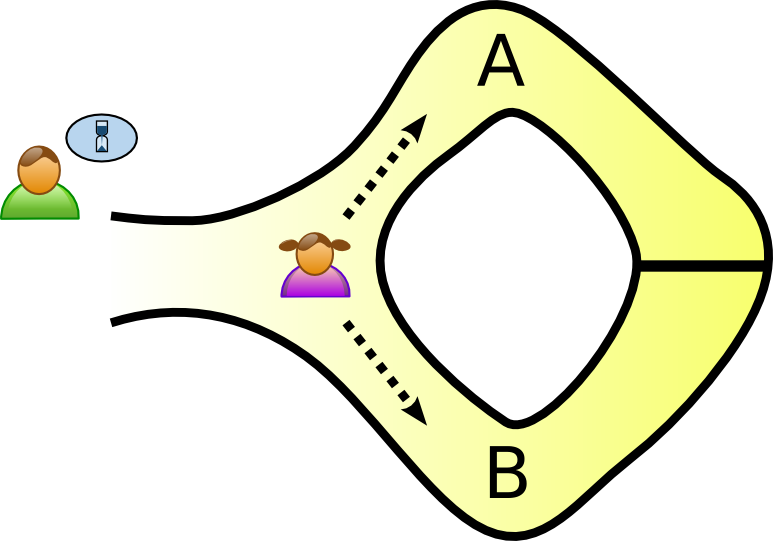
\includegraphics[width=0.35\textwidth]{img/zero_knowledge1.png}
    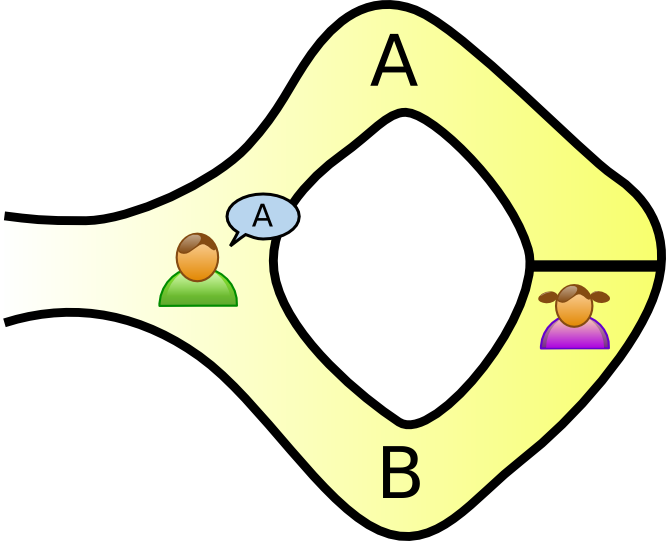
\includegraphics[width=0.3\textwidth]{img/zero_knowledge2.png}
    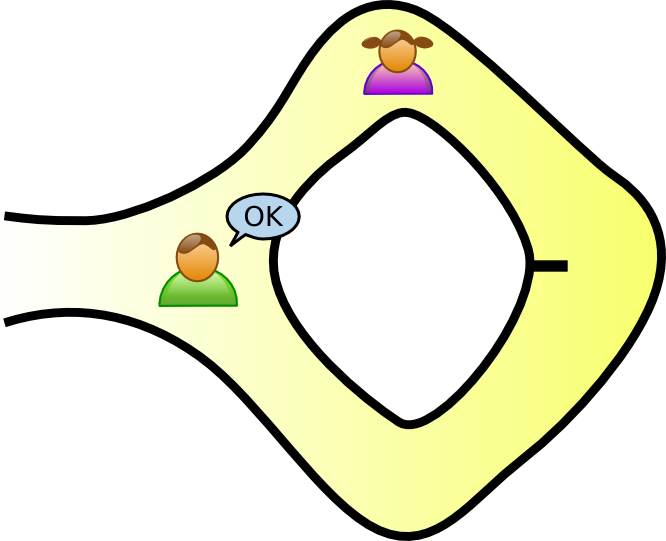
\includegraphics[width=0.3\textwidth]{img/zero_knowledge3.png}
    \caption{Peggy è in grado di dimostrare a Victor di conoscere l'informazione senza rivelarla,
    dimostrando di riuscire ad uscire dall'estremità corretta del labirinto.}
\end{figure}
Se Victor seguisse Peggy, potrebbe imparare l'informazione, quindi Peggy deve essere in grado di 
dimostrare di conoscere l'informazione senza che Victor possa impararla.
Se invece Victor andasse dalla parte opposta, non imparerebbe nulla, ma sarebbe in grado di 
dimostrare a terzi che Peggy conosce l'informazione, filmando l'apertura della porta.

Quello che si può fare è far scegliere da Peggy una delle due direzioni attraverso il lancio 
di una moneta, dopo che Peggy ha raggiunto la direzione decisa attraverso il lancio della moneta,
Victor raggiunge lo stesso punto di partenza di Peggy e lancia 
la moneta per decidere la direzione che Peggy deve prendere, Peggy deve quindi prendere la direzione
decisa da Victor. Se Peggy conosce l'informazione, riuscirà sempre a prendere la direzione decisa
da Victor, altrimenti con probabilità $\frac{1}{2}$ non sarà in grado di prendere la direzione
decisa da Victor.
Per abbassare la probabilità di errore, si può ripetere il protocollo più volte, in questo modo
se Peggy non conosce l'informazione, la probabilità di errore sarà $\frac{1}{2^k}$, dove $k$ è il
numero di volte che si ripete il protocollo.

Victor non sarà in grado di dimostrare a terzi che Peggy conosce l'informazione, poiché dall'ipotetico 
filmato che Victor potrebbe girare, non si capirebbe se i due hanno deciso la direzione in anticipo
o se Peggy conosce l'informazione, essendo che si vedrebbe solo la comunicazione della direzione da parte di Victor e
l'uscita di Peggy dalla direzione decisa da Victor.
\section{Classe \texttt{P} e \texttt{NP}}
Un problema decisionale $Q$ appartiene a \texttt{P} se esiste una macchina di Turing
deterministica (\textit{o equivalente}) che, in tempo polinomiale rispetto alla dimensione dell'input,
può risolvere il problema $Q$.

Un problema decisionale $Q$ appartiene a \texttt{NP} se e solo se esiste una macchina di Turing deterministica
(\textit{o equivalente}) che, in tempo polinomiale rispetto alla dimensione dell'input, può verificare soluzioni
proposte per ogni istanza $x$ di $Q$. 

\begin{theorem}
    Un linguaggio $\mathcal{L} \in \texttt{NP}$ se e solo se esiste un linguaggio 
    $\mathcal{L'}$ appartenente alla classe \texttt{P} tale che $\forall x \in \mathcal{L}$, esiste
    un certificato $y$ tale che $(x,y) \in \mathcal{L'}$.
\end{theorem}
In generale quindi dimostrare un teorema è più difficile che verificare che un teorema sia vero.
Se volessimo dimostrare che verificare non è più difficile che dimostrare potremmo farlo dando una 
potenza di calcolo limitata a chi verifica e una potenza di calcolo illimitata a chi dimostra.
\section{Interactive proof system}
Un \textbf{interactive proof system} è una coppia di algoritmi (\textit{macchine di Turing}) $(P,V)$, tali 
che $P$ ha potenza di calcolo illimitata e $V \in \texttt{PPT}$. $P$ e $V$ interagiscono scambiandosi 
messaggi e alla fine $V$ deve decidere se accettare o rifiutare l'input $x$.

Un linguaggio $\mathcal{L}$ ammette un \texttt{IPS} (\textit{Interactive Proof Space}) se
esistono due algoritmi, \(P\) e \(V\), tali che:

\[
\forall x \in \mathcal{L} \quad \mathcal{P}[(P,V) \text{ accetta } x] > \frac{2}{3}
\] 

\[
\forall x \notin \mathcal{L} \quad \forall P' \quad \mathcal{P}[(P',V) \text{ accetta } x] \leq \frac{1}{3}
\]

La classe di linguaggi che ammettono un \texttt{IPS} si chiama \texttt{IP}. Quindi, un linguaggio $\mathcal{L}$
appartiene a \texttt{IP} se ammette un \texttt{IPS}.

Inoltre, si ha l'inclusione di classi di complessità:

\[
\texttt{NP} \subseteq \texttt{IP}
\]

Il seguente teorema afferma l'equivalenza tra le classi di complessità
\texttt{IP} e \texttt{PSPACE}:

\begin{theorem}
    \texttt{IP} $=$ \texttt{PSPACE}
\end{theorem}
\begin{proof}
La dimostrazione di questa equivalenza coinvolge la costruzione di trasformazioni tra le classi \texttt{IP} e \texttt{PSPACE}
in entrambe le direzioni.
Per dimostrare \( \texttt{IP} \subseteq \texttt{PSPACE} \), si mostra che ogni problema risolvibile in modo interattivo
in tempo polinomiale ha anche una soluzione in spazio polinomiale.
La direzione opposta, \( \texttt{PSPACE} \subseteq \texttt{IP} \), richiede la costruzione di un protocollo interattivo
che possa simulare una macchina di Turing con spazio limitato e risolvere il problema in modo interattivo.
Pertanto, si conclude che \( \texttt{IP} \) e \( \texttt{PSPACE} \) sono equivalenti in termini di potenza computazionale.
\end{proof}
\subsection{Quadratic non-residuosity}
Tale problema è un problema appartenente alla classe di problemi \texttt{CO-NP}, perché verificare che un numero 
sia effettivamente un quadrato è un problema di \texttt{NP} e il certificato che mostra che un numero è un quadrato è
una delle due radici quadrate del numero.

Abbiamo un numero in $\mathbb{Z}_n^*$ che non è un quadrato e vogliamo costruire un interactive proof system
per dimostrare che non è un quadrato.

L'idea alla base è che se $x$ non è un quadrato, allora moltiplicando $x$ per un quadrato, il risultato non sarà un quadrato.

L'input del problema è la coppia $(n,x)$, e l'output accetta se $x$ è un non-residuo quadratico in $\mathbb{Z}_n^*$.
Victor manda a Peggy $w_1, w_2, \dots, w_l$ dove:
\[
  w_i = \begin{cases}
    z_i^2 & \text{con } z_i \in_R \mathbb{Z}_n^* \text{ se }b_i = 0 \text{ dove }b_i \in_R \{0,1\} \\
    x \cdot z_i^2 & \text{altrimenti}  
    \end{cases}
\]
Peggy invia a Victor la sequenza $c_1, c_2, \dots, c_l$ dove:
\[
  c_i = \begin{cases}
    0 & \text{se }w_i \text{ è un quadrato} \\
    1 & \text{altrimenti}
    \end{cases}
\]
Se $x$ non è un quadrato, allora $w_i$ è un quadrato se e solo se $b_i = 0$ e
non è un quadrato se e solo se $b_i = 1$. Victor accetta solo se $c_i = b_i$ per ogni $i$.
La se Peggy non conosce la soluzione, la probabilità che Victor accetti è $\frac{1}{2^l}$, 
mentre se la conosce la probabilità è $1$.
L'idea intuitiva è che la capacità di rispondere coincida con la conoscenza del segreto, in questo caso 
visto che nel mondo reale prover con potenza di calcolo illimitata non esistono, e visto 
che Peggy riesce a rispondere alle domande di Victor, allora Peggy conosce la fattorizzazione 
di $n$.
\subsection{Graph non-isomorphism}
Abbiamo due grafi $G_1$ e $G_2$ e vogliamo costruire un interactive proof system per dimostrare che non sono isomorfi,
$G_1 \not\simeq  G_2$. Ricordiamo che due grafi sono isomorfi se esiste una funzione biunivoca tra i vertici dei due
grafi che preserva gli archi.

\begin{figure}[H]
    \centering
        \begin{tikzpicture}
            \begin{scope}[every node/.style={circle,thick,draw}]
                \node (A) at (0,0) {A};
                \node (B) at (2.5,1) {B};
                \node (C) at (5,0) {C};
                \node (D) at (2.5,-3) {D};
                \node (E) at (0,2) {E};
                \node (F) at (5,2) {F} ;
            \end{scope}
            
            \begin{scope}[>={Stealth[black]},
                          every edge/.style={draw=black,very thick}]
                \path [-] (A) edge node {} (E);
                \path [-] (E) edge node {} (F);
                \path [-] (E) edge node {} (B);
                \path [-] (B) edge node {} (D);
                \path [-] (D) edge node {} (F);
                \path [-] (F) edge node {} (C);
                \path [-] (C) edge node {} (D);
                \path [-] (C) edge node {} (F);
                \path [-] (B) edge node {} (C); 
            \end{scope}
        \end{tikzpicture}
        \begin{tikzpicture}
            \begin{scope}[every node/.style={circle,thick,draw}]
                \node (A) at (0,0) {A};
                \node (B) at (0,3) {B};
                \node (C) at (2.5,4) {C};
                \node (D) at (2.5,1) {D};
                \node (E) at (2.5,-3) {E};
                \node (F) at (5,3) {F} ;
            \end{scope}
            
            \begin{scope}[>={Stealth[black]},
                          every edge/.style={draw=black,very thick}]
                \path [-] (A) edge node {} (B);
                \path [-] (B) edge node {} (C);
                \path [-] (D) edge node {} (C);
                \path [-] (D) edge node {} (E);
                \path [-] (D) edge node {} (F);
                \path [-] (C) edge node {} (F);
                \path [-] (E) edge node {} (F); 
                \path [-] (B) edge[bend right=60] node {} (E); 
            \end{scope}
        \end{tikzpicture}
    \caption{Esempio di due grafi isomorfi}
\end{figure}

\begin{tcolorbox}[title=Isomorfismo di grafi]
    Due grafi sono isomorfi, quando esiste un mapping biunivoco, che preserva 
    gli archi, tra i vertici dei due grafi.
\end{tcolorbox}

$V$ sceglie un grafo $G\in_R \{G_1, G_2\}$ e lo permuta casualmente in $G'$. $V$ invia $G'$ a $P$ e $P$ 
stabilisce se $G'$ è isomorfo a $G_1$ o $G_2$ e invia il risultato a $V$. $V$ accetta se $P$ indovina correttamente.

Il fatto che $P$ sia in grado di rispondere è dovuto al fatto che abbia potenza di calcolo illimitata e non 
è dovuto al fatto che vi siano informazioni trapdoor. 

Vorremo arrivare al punto che $V$ non impari nulla di più se non il non isomorfismo tra i grafi, poiché 
potrebbe esistere un $V$ che ha come obiettivo di sapere qualcosa in più, come ad esempio capire se $G_2$
è isomorfo a un altro grafo $G_3$. Per farlo parte dall'istanza di $G_1$ e $G_2$ per interagire con $P$, 
e la prima richiesta sarà proprio $G_3$. Usando quindi $P$ per risolvere problemi di cui non ha 
l'informazione. 

L'idea è che $V$ avrebbe potuto simulare l'interazione con $P$ senza interagire con $P$ stesso.
Se $P$ e $V$ interagiscono vengono prodotti una serie di messaggi, che in realtà sono una sequenza casuale,
perché $P$ e $V$ sono algoritmi stocastici, dove vengono effettuate scelte casuali, producendo quindi
una \textbf{misura di probabilità} su sequenze di messaggi chiamata $\texttt{view}(P,V,x,h)$. 
Con $h$, che rappresenta l'\textit{hint}, si vuole catturare l'idea che qualcuno possa fornire informazioni 
aggiuntive a $V$ per aiutarlo a rispondere alle domande di $P$.

\begin{tcolorbox}
    Diciamo che $P,V$ è zero-knowledge se per ogni $V'\in \texttt{PPT}$ esiste un simulatore $M \in \texttt{PPT}$
    tale che $M(P,V',x,h) = \texttt{view}(P,V,x,h)$. In grado quindi di produrre una sequenza di messaggi
    distribuite esattamente come quelle di \texttt{view}.   
\end{tcolorbox} 
\subsection{Ciclo hamiltoniano}
\begin{tcolorbox}
    Un ciclo hamiltoniano è un ciclo che passa per tutti i vertici di un grafo una e una sola volta.
\end{tcolorbox}
\begin{figure}[H]
    \centering
        \begin{tikzpicture}
            \begin{scope}[every node/.style={circle,thick,draw}]
                \node (A) at (0,0) {A};
                \node (B) at (2.5,1) {B};
                \node (C) at (5,0) {C};
                \node (D) at (2.5,-3) {D};
                \node (E) at (0,2) {E};
                \node (F) at (5,2) {F} ;
            \end{scope}
            
            \begin{scope}[>={Stealth[black]},
                          every edge/.style={draw=black,very thick}]
                \path [-] (A) edge node {} (E);
                \path [-] (E) edge node {} (F);
                \path [-] (E) edge node {} (A);
                \path [-] (B) edge node {} (D);
                \path [-] (F) edge node {} (C);
                \path [-] (C) edge node {} (D);
                \path [-] (C) edge node {} (F);
                \path [-] (B) edge node {} (C);
                \path [-] (B) edge node {} (A);
            \end{scope}
        \end{tikzpicture}
    \caption{Esempio di un ciclo hamiltoniano}
\end{figure}
Per farlo $P$ permuta $G$ per ottenere $H$, grafo isomorfo a $G$ e codifica tutti i bit della matrice di adiacenza
di $H$ con bit commitment, e sia $H'$ il risultato. $P$ invia $H'$, sapendo che il dato inviato non rivela alcuna 
informazione circa i bit al suo interno. $V$ lancia una moneta per decidere se chiedere a $P$ l'evidenza 
che $G \simeq H$ o l'evidenza che $H$ ammette un ciclo hamiltoniano. 
$P$ obbedisce e nel caso in cui $V$ abbia chiesto l'evidenza che $G \simeq H$ allora rivela $H$ e l'isomorfismo
tra $G$ e $H$ (\textit{se uno ammette ciclo hamiltoniamo, lo ammettee anche l'altro}).
Se invece $V$ ha chiesto l'evidenza che $H$ ammette un ciclo hamiltoniano, scopre solo i bit di $H$ che 
costituiscono un ciclo hamiltoniano.

Se $G$ non ammette ciclo hamiltoniamo allora il grafo $H$ inviato dal prover, non è possibile che sia sia isomorfo 
a $G$ e che ammetta un ciclo hamiltoniano. Se è isomorfo a $G$, visto che $G$ non ammette ciclo hamiltoniano, allora 
$H$ non può ammetterlo. In quel caso il verifier saprà solamente fornire la risposta ad una delle due domande.
Visto che il verifier sceglie le domande casualmente, con probabilità $\frac{1}{2}$ il verifier sceglierà la domanda
a cui il prover non sa rispondere.
Di conseguenza se $G$ ammette ciclo hamiltoniano, il prover risponderà sempre in qualsiasi caso e quindi 
risponderà correttamente con probabilità $1$.
\subsection{Costruzione del simulatore $M$}
Vogliamo far si che $V$ non possa utilizzare l'interazione con $V$ per convincere terzi.
Per farlo scegliamo casualmente la domanda di $V$, se la domanda che fa $V$ è di dimostrare che $G \simeq H$,
allora costruiamo $H'$ secondo il protocollo.
\pseudocodeblock{
\begin{tikzpicture}
  \node[bob, minimum size=2cm,label=below:{Prover}] (Prover) {};
\end{tikzpicture}
\<\<
\begin{tikzpicture}
  \node[bob, mirrored, minimum size=2cm, label=below:{Verifier}] (Verifier) {};
\end{tikzpicture}
\\[0.1\baselineskip][\hline] \\[-0.5\baselineskip]
\text{Codifica }H' \text{ con bit commitment}\<\<  \\
\< \sendmessageright*{H'}\< \\
\<\sendmessageleft*{\text{Dimostra che } G \simeq H}\<\\
\<\sendmessageright*{\text{Rivela } H \text{ e }G \simeq H}\<\\
}
Se invece la domanda è di dimostrare che $H$ ammette un ciclo hamiltoniano, allora $P$ invia $H'$ 
bit commitment del grafo \textbf{completo}, scegliendo una permutazione casuale dei nodi come ciclo.
\pseudocodeblock{
\begin{tikzpicture}
    \node[bob, minimum size=2cm,label=below:{Prover}] (Prover) {};
\end{tikzpicture}
    \<\<
\begin{tikzpicture}
    \node[bob, mirrored, minimum size=2cm, label=below:{Verifier}] (Verifier) {};
\end{tikzpicture}
\\[0.1\baselineskip][\hline] \\[-0.5\baselineskip]
\text{Codifica }H' \text{ con bit commitment}\<\<  \\
\< \sendmessageright*{H'}\< \\
\<\sendmessageleft*{H \text{ hamiltoniano}}\<\\
\text{Codifica $H'$ con bit commitment} \<\< \\
\text{del grafo completo con un ciclo} \<\< \\
\text{hamiltoniamo casuale.} \<\< \\
\<\sendmessageright*{\text{Invia } H'}\<\\
}
La distribuzione di probabilità delle domande che può effettuare il prover è di $\frac{1}{2}$ per ciascuna domanda.
La distribuzione di probabilità delle risposte che può dare il prover è corretta nel primo caso, è infatti 
dovuta alla permutazione casuale che può assumere il grafo. Nel secondo caso invece si tratta di una permutazione 
casuale dei nodi del grafo $H'$.
Permutando un grafo con ciclo hamiltoniano, il ciclo diventa una permutazione 
dei nodi del grafo, quindi qualunque permutazione ha la stessa probabilità di essere un ciclo hamiltoniamo, quindi 
la probabilità 
che una determinata permutazione sia un ciclo hamiltoniano è sempre la stessa

Nel primo caso la misura di probabilità è sempre la stessa, nel secondo caso invece la misura di probabilità è diversa.

Un qualunque terzo osservatore che abbia potenza di calcolo polinomiale
che osserva l'interazione tra $P$ e $V$, non può distinguere
l'interazione reale che avviene tra $P$ e $V$ da un'interazione simulata tra $P$ e $V$. Un osservatore che osserva $H'$
fornito dalla seconda interazione (\textit{ovvero quello che ha la permutazione casuale dei nodi del grafo completo}),
non riesce a capire che l'$H'$ inviato dal verifier è la matrice di adiacenza di un grafo completo o meno.

Supponendo di avere un algoritmo $\mathcal{D} \in \texttt{PPT}$ che campiona i messaggi tra \texttt{View} e \texttt{M}
e che riesce a distinguere tra l'interazione reale e quella simulata, allora siamo in grado di distinguere tra 
il bit commitment di un grafo con ciclo hamiltoniamo da il bit commitment di un grafo completo, ma ciò si traduce 
in un algoritmo che risolve il problema del bit commitment, che è un problema non risolvibile in \texttt{PPT}.

Quello che viene effettivamente visto esternamente è la distribuzione di probabilità tra le domande e le risposte, ma 
non viene effettivamente vista la differenza tra le due versioni di $H'$.
\begin{tcolorbox}[title = Perfect Zero Knowledge]
    In questo caso le due distribuzioni di probabilità sono identiche, ovvero:
    \[
      \texttt{view}(P,V,x,h) = M(P,V,x,h)
    \]
\end{tcolorbox}
\begin{tcolorbox}[title = Statistical Zero Knowledge]
    In questo caso la differenza tra le due distribuzioni di probabilità è trascurabile, ovvero
    non esiste un algoritmo \texttt{PPT} che riesce a distinguere tra le due distribuzioni di probabilità.
    \[
      \sum_\omega \bigg| \texttt{view}(P,V,x,h)(\omega) - M(P,V,x,h)(\omega)  \bigg| \leq k^{-\omega(1)}
    \]
\end{tcolorbox}
\begin{tcolorbox}[title = Computational Zero Knowledge]
    In questo caso le due misure di probabilità sono polinomialmente indistinguibili, ovvero
    $\forall \mathcal{D} \in \texttt{PPT}$ sia $\mathcal{P}_k^{\mathcal{D}, \mathcal{V}}$ la
    probabilità che $\mathcal{D}$ restituisca $1$ campionando da \texttt{view} e 
    sia $\mathcal{P}_k^{\mathcal{D}, \mathcal{M}}$ la probabilità che $\mathcal{D}$
    restituisca $1$ campionando da $M$,
    \[
        \bigg| \mathcal{P}_k^{\mathcal{D}, \mathcal{V}} - \mathcal{P}_k^{\mathcal{D}, \mathcal{M}} \bigg| \leq k^{-\omega(1)}
    \]
    Non esiste un algoritmo \texttt{PPT} che riesce a distinguere tra le due distribuzioni di probabilità.
\end{tcolorbox}
\subsection{Tre colorabilità di un grafo}
\begin{figure}[H]
    \centering
    \begin{tikzpicture}
        \begin{scope}[every node/.style={circle,thick,draw}]
            \node[fill=blue!30] (A) at (0,0) {A};
            \node[fill=green!30] (B) at (2.5,1) {B};
            \node[fill=red!30] (C) at (5,0) {C};
            \node[fill=green!30] (D) at (2.5,-1) {D};
            \node[fill=red!30] (E) at (0,2) {E};
            \node[fill=blue!30] (F) at (5,2) {F} ;
        \end{scope}
        
        \begin{scope}[>={Stealth[black]},
                      every edge/.style={draw=black,very thick}]
            \path [-] (A) edge node {} (E);
            \path [-] (A) edge node {} (C);
            \path [-] (A) edge node {} (D);
            \path [-] (E) edge node {} (B);
            \path [-] (E) edge node {} (F);
            \path [-] (B) edge node {} (E);
            \path [-] (B) edge node {} (F);
            \path [-] (F) edge node {} (C);
            \path [-] (C) edge node {} (D);
        \end{scope}
    \end{tikzpicture}
\end{figure}
Nel contesto della dimostrazione della tre-colorabilità di un grafo senza rivelare la
colorazione effettiva dei nodi, si adotta un protocollo computational zero knowledge.
L'obiettivo è dimostrare che un grafo può essere colorato con tre colori in modo tale che
nodi adiacenti abbiano colori distinti, senza mai rivelare la specifica colorazione adottata.

Il protocollo inizia con un accordo tra il prover e il verifier su un grafo G. Il prover si
impegna a dimostrare la tre-colorabilità del grafo senza rivelare direttamente la colorazione.

Per mantenere la confidenzialità, il prover sceglie casualmente una permutazione tra tre colori
(\textit{ad esempio, rosso, verde e blu}) senza rivelarla al verifier. Questa permutazione sarà
utilizzata per colorare i nodi del grafo.

Il verifier, a sua volta, sfida il prover selezionando casualmente due nodi adiacenti, A e B,
e richiede la rivelazione dei colori associati secondo la permutazione scelta. Il prover risponde
rivelando i colori senza svelare la permutazione effettiva. Il verifier può verificare se i colori
sono diversi, confermando così la corretta tre-colorabilità del grafo.
Questo processo può essere ripetuto per diverse coppie di nodi adiacenti, ma la casualità nella
selezione delle sfide impedisce al verifier di dedurre la permutazione specifica attraverso tentativi
ripetuti.

Il prover, per evitare la possibile deduzione della permutazione da parte del verifier attraverso
esperimenti multipli, permuta casualmente i colori ad ogni sfida successiva. In questo modo, il verifier
non può accumulare informazioni utili per dedurre la tre-colorabilità del grafo.

Alla conclusione del protocollo, se il prover ha superato con successo tutte le sfide, il verifier acquisisce
la convinzione della tre-colorabilità del grafo, senza mai venire a conoscenza della specifica
permutazione dei colori utilizzata dal prover. Questo dimostra l'efficacia della computational zero knowledge
nel preservare la riservatezza della colorazione dei nodi.
\section{Ripetizione parallela della zero knowledge}
Per come abbiamo definito la zero knowledge, il protocollo può essere ripetuto più volte
eseguendo arbitrariamente la sequenza di \textit{challenge, question, response}.
Se il protocollo seguisse uno schema parallelo di esecuzione, ovvero se il verifier 
ponesse più domande in parallelo, il prover potrebbe rispondere a tutte le domande
con una singola risposta, senza dover ripetere il protocollo per ogni domanda.
\pseudocodeblock{
\begin{tikzpicture}
  \node[bob, minimum size=2cm,label=below:{Prover}] (Prover) {};
\end{tikzpicture}
\<\<
\begin{tikzpicture}
  \node[bob, mirrored, minimum size=2cm, label=below:{Verifier}] (Verifier) {};
\end{tikzpicture}
\\[0.1\baselineskip][\hline] \\[-0.5\baselineskip]
\<\<\text{Challenge }c_1, c_2, \dots c_l\< \\
\<\sendmessageleft*{\text{Question }q_1, q_2,\dots,q_l}\<\\
\<\sendmessageright*{\text{Response }r_1,r_2,\dots,r_l}\<\\
}
Per uno schema sequenziale, dove gli eventi sono mutuamente indipendenti, è possibile creare
misure di probabilità che risultano indistinguibili dall'originale. Tuttavia, la zero knowledge
proof in uno schema parallelo presenta delle sfide. Questo è evidente definendo $q_1, q_2, \dots, q_l$
come una funzione hash unidirezionale $H(c_1, c_2, \dots, c_l)$. Nel contesto dello schema parallelo,
la tecnica per simulare la sequenza di messaggi diventa impraticabile. La difficoltà principale risiede
nella necessità di invertire la funzione hash, che è di tipo unidirezionale, al fine di costruire le
challenge $c_1, c_2, \dots, c_l$ per la simulazione.

Una proof zero knowledge in cui il verifier pone domande al prover sulla base di una funzione hash 
one way applicata alle challenge, è qualcosa che riesce a convincere terze parti che il prover
conosce la soluzione.
\section{Non interactive zero knowledge}
La non interactive zero knowledge è una variante della zero knowledge proof in cui qualcuno 
conosce il segreto senza rivelare chi sia, non rivelando nessuna informazione circa il segreto
stesso. L'aspetto cruciale delle non interactive zero knowledge è la capacità di dimostrare
la conoscenza di un segreto in modo autonomo e senza rivelare
dettagli sensibili, rendendole particolarmente utili in applicazioni decentralizzate come le blockchain.
\end{document}
